
%!TeX spellcheck = en-US

\documentclass[
    12pt, % The default document font size, options: 10pt, 11pt, 12pt
    %oneside, % Two side (alternating margins) for binding by default, uncomment to switch to one side
    % greek, % ngerman for German
    singlespacing, % Single line spacing, alternatives: onehalfspacing or doublespacing
    %draft, % Uncomment to enable draft mode (no pictures, no links, overfull hboxes indicated)
    %nolistspacing, % If the document is onehalfspacing or doublespacing, uncomment this to set spacing in lists to single
    liststotoc, % Uncomment to add the list of figures/tables/etc to the table of contents
    %toctotoc, % Uncomment to add the main table of contents to the table of contents
    %parskip, % Uncomment to add space between paragraphs
    %nohyperref, % Uncomment to not load the hyperref package
    headsepline, % Uncomment to get a line under the header
    %chapterinoneline, % Uncomment to place the chapter title next to the number on one line
    %consistentlayout, % Uncomment to change the layout of the declaration, abstract and    acknowledgements pages to match the default layout
]{DoctoralThesis} % The class file specifying the document structure

\usepackage[utf8]{inputenc} % Required for inputting international characters
\usepackage[T1]{fontenc} % Output font encoding for international characters
\usepackage{mathpazo} % Use the Palatino font by default

% ----------------------------------------------------------------------------------------------------- 
% --------------------------- REQUIREMENT FOR SUPPORTING GREEK LANGUAGE ------------------------------
% ----------------------------------------------------------------------------------------------------- 
\usepackage{fontspec}
\newfontfamily\greekfont{FreeSerif}
%\setmainfont{FreeSerif}[BoldFont=FreeSerifBold]
%\setseriffont{FreeSerifBold}
%\setsansfont{FreeSans}
%\setmonofont{FreeMono}

\usepackage{polyglossia}
\setdefaultlanguage{english}
\setotherlanguage{greek}

% I AM NOT SURE I NEED THIS GEOMENTRY... geomfds
\geometry{
	paper=a4paper, % Change to letterpaper for US letter
	inner=2.5cm, % Inner margin
	outer=3.8cm, % Outer margin
	bindingoffset=.5cm, % Binding offset
	top=2.5cm, % Top margin
	bottom=2.5cm, % Bottom margin
	%showframe, % Uncomment to show how the type block is set on the page
}

\usepackage{natbib}
\usepackage{mathptmx}
\usepackage{amsmath}
\usepackage{amsmath}
\DeclareMathOperator*{\argminA}{arg\,min}
\usepackage{amsfonts}
\usepackage{amssymb}
\usepackage[dvips,dvipdfm,pdftex]{graphicx}
\usepackage{pgfplotstable}
\usepackage{pgfplots}
\pgfplotsset{compat=newest}
\usepackage{array}
\usepackage{booktabs}
\usepackage{morefloats}
\usepackage{etex}
\usepackage{listings}
\usepackage{float}
\usepackage{epstopdf}
\usepackage{multirow}
\usepackage[section]{placeins}
\usepackage[ruled,linesnumbered,resetcount,algochapter]{algorithm2e}
\usepackage{mathtools}
\usepackage{pifont} % for \cmark and \xmark symbols
\usepackage{graphics}
\usepackage{adjustbox}

\newcommand{\cmark}{\ding{51}}%
\newcommand{\xmark}{\ding{55}}%

\DeclarePairedDelimiter\floor{\lfloor}{\rfloor}

\newtheorem{definition}{Definition}

\usepackage[backend=bibtex,style=authoryear,natbib=true]{biblatex} % Use the bibtex backend with the authoryear citation style (which resembles APA)
\addbibresource{PhD_Thesis.bib} % The filename of the bibliography
\usepackage[autostyle=true]{csquotes} % Required to generate language-dependent quotes in the bibliography

%----------------------------------------------------------------------------------------
%	THESIS INFORMATION
%----------------------------------------------------------------------------------------

\thesistitle{Open-set Web Genre Identification}
\supervisor{Efstathios \textsc{Stamatatos}}
% \examiner{} % Your examiner's name, this is not currently used anywhere in the template, print it elsewhere with \examname
\degree{Doctor of Philosophy} % Your degree name, this is used in the title page and abstract, print it elsewhere with \degreename
\author{Dimitrios \textsc{Pritsos}}
\addresses{} % Your address, this is not currently used anywhere in the template, print it elsewhere with \addressname
\subject{Computer Science} % Your subject area, this is not currently used anywhere in the template, print it elsewhere with \subjectname
\keywords{} % Keywords for your thesis, this is not currently used anywhere in the template, print it elsewhere with \keywordnames
\university{\href{http://www.aegean.gr}{University of the Aegean}} % Your university's name and URL, this is used in the title page and abstract, print it elsewhere with \univname
% \department{\href{http://department.university.com}{Department or School Name}} % Your department's name and URL, this is used in the title page and abstract, print it elsewhere with \deptname
% \group{\href{http://researchgroup.university.com}{Research Group Name}} % Your research group's name and URL, this is used in the title page, print it elsewhere with \groupname
% \faculty{\href{http://faculty.university.com}{Faculty Name}} % Your faculty's name and URL, this is used in the title page and abstract, print it elsewhere with \facname

\AtBeginDocument{
\hypersetup{pdftitle=\ttitle} % Set the PDF's title to your title
\hypersetup{pdfauthor=\authorname} % Set the PDF's author to your name
\hypersetup{pdfkeywords=\keywordnames} % Set the PDF's keywords to your keywords
}

\begin{document}

\frontmatter % Use roman page numbering style (i, ii, iii, iv...) for the pre-content pages

\pagestyle{plain} % Default to the plain heading style until the thesis style is called for the body content

%----------------------------------------------------------------------------------------
%	TITLE PAGE
%----------------------------------------------------------------------------------------

\begin{titlepage}
\begin{center}

\vspace*{.06\textheight}
{\scshape\LARGE \univname\par}\vspace{1.5cm} % University name
\textsc{\Large Doctoral Thesis}\\[0.5cm] % Thesis type

\HRule \\[0.4cm] % Horizontal line
{\huge \bfseries \ttitle\par}\vspace{0.4cm} % Thesis title
\HRule \\[1.5cm] % Horizontal line

\begin{minipage}[t]{0.4\textwidth}
\begin{flushleft} \large
\emph{Author:}\\
\href{http://www.aegean.gr}{\authorname} % Author name - remove the \href bracket to remove the link
\end{flushleft}
\end{minipage}
\begin{minipage}[t]{0.4\textwidth}
\begin{flushright} \large
\emph{Supervisor:} \\
\href{http://www.aegean.gr}{\supname} % Supervisor name - remove the \href bracket to remove the link
\end{flushright}
\end{minipage}\\[3cm]

\vfill

\large A thesis submitted in fulfillment of the requirements\\ for the degree of \degreename\\[0.3cm] % University requirement text
at the\\[0.4cm]
\groupname\\\deptname{Dept. of Information and Communication Systems Eng.}\\[2cm] % Research group name and department name

\vfill

{\large \today}\\[4cm] % Date
%\includegraphics{Logo} % University/department logo - uncomment to place it

\vfill
\end{center}
\end{titlepage}


%----------------------------------------------------------------------------------------
%	ADVISING COMMITTEE
%----------------------------------------------------------------------------------------
\section*{Advising Committee}

\begin{center}
\vspace*{.06\textheight}

\HRule\\
Efstathios Stamatatos, Supervisor\\
Professor, University of the Aegean,\\
Greece\\

\HRule\\
George Vouros, Advisor\\
Professor, University of Piraeus,\\
Greece\\

\HRule\\
Yannis Tzitzikas, Advisor\\
Associate Professor, University of Crete,\\
Greece\\

\HRule\\

\end{center}

\newpage


%----------------------------------------------------------------------------------------
%	ADVISING COMMITTEE
%----------------------------------------------------------------------------------------
\section*{Examining Committee}

\begin{center}
\vspace*{.06\textheight}

\HRule\\
Efstathios Stamatatos\\
Professor, University of the Aegean,\\
Greece\\

\HRule\\
George Vouros\\
Professor, University of Piraeus,\\
Greece\\

\HRule\\
Yannis Tzitzikas\\
Associate Professor, University of Crete,\\
Greece\\

\HRule\\
Christos Goumopoulos\\
Assistant Professor, University of the Aegean,\\
Greece\\

\HRule\\
Ergina Kavallieratou\\
Associate Professor, University of the Aegean,\\
Greece\\

\HRule\\
Alexios Kaporis\\
Assistant Professor, University of the Aegean,\\
Greece\\

\HRule \\
Andreas Papasaliouras\\
Assistant Professor, University of the Aegean,\\
Greece\\

\HRule \\[0.3cm] % Horizontal line

\end{center}


\newpage


%----------------------------------------------------------------------------------------
%	DECLARATION OF AUTHORSHIP
%----------------------------------------------------------------------------------------

\section*{Declaration}
I declare that I am the sole author of this thesis and that I have not used any source other than those listed in the bibliography and Identified as references. I further declare that I have not submitted this thesis at any other institution in order to obtain a degree.

\newpage

%----------------------------------------------------------------------------------------
%   DEDICATION
%----------------------------------------------------------------------------------------

\section*{Dedication}
To my family.

\newpage
 

\section*{Acknowledgements}
I would like to thank my supervisor, Professor Efstathios Stamatatos for being my teacher. A teacher with excellent academic skills who has been guiding me into innovative and novel research paths. A teach eager for knowledge who has been inspiring me with his patience.

\subsection*{Timeline Acknowledgements}
I would like to thank few people who I believe they where very inspiring for my academic choices. Giorgos Vargiadakis (elementary school), Giorgos Dimitropoulos (highschool), Nikos Mavrelis (senior highschool) who inspired the my love for mathematics and philosophical/critical thinking. I would also like to thank my undergraduate professors Christos Skourlas and Nikos Vassilas for helping pursuit my academic goals with their guidance and inspiring lectures. I finally would like to thank my postgraduate supervisor Ulrich Nehmzow for his inspiring lectures in (robotics) research methodology.

I would like to thank my three close friends Vasilis Paraskevopoulos, Eleftherios Garifalidis and Vasilis Dimitriadis for their support when work and studies where coming in conflict in respect of my time management. I also would like to thank them for their time when they used to listening for my "PhD stories" and for their analytical thinking always being useful for my decisions. I would also like to thank my fiancee Vasiliki Charalampopoulou who has been with me since the early days of my PhD studies.

Last but not least I would like to thank my parents who taught me working tirelessly for my goals. Antonis, my father, who is my very first teacher in analytic thinking and Antonia, my mother, who inspired me the love for knowledge. 

\subsection*{Scholarships Acknowledgements}
I would like to thank \textit{The State Scholarships Foundation (I.K.Y.) of Greece} for the scholarships No.5706/27-01-2010, granted to me for the first three (3) year of my PhD studies.


\newpage



%----------------------------------------------------------------------------------------
%	ABSTRACT PAGE
%----------------------------------------------------------------------------------------
\begin{abstract}
\addchaptertocentry{\abstractname} % Add the abstract to the table of contents

World wide web is constantly increasing and people use information in web-pages for everyday activities. There is an emerging need for facilitating access in this huge repository in a seamless way that is in accordance with users' understanding. Genre is an important factor to characterize the properties of web-pages. Web genres (e.g., blogs, e-shop, FAQs, etc.) refer to the form, structure, and communicative purpose of web-pages rather than their topic. Web Genre Identification (WGI) provides a means to improve effectiveness of information retrieval systems by allowing sophisticated queries combining topic and genre information and ranking/grouping search results according to genre. Specialized document collections can be compiled by adopting genre-aware focused crawling. The credibility assessment of web-pages can be significantly enhanced given that information about their genre is available. Cyber-security applications like anti-phishing can also be enhanced by incorporating genre of web-pages. In case natural language technology tools should be applied to the textual part of web-pages, knowing their genre allows the selection of appropriate tools that have been trained to handle similar documents. 

Existing work in WGI largely follows the closed-set classification scenario where given a genre palette and training examples for each known genre the task is to assign every new web-page to one of the known genres. However, this does not fit most of applications related to WGI. There is no consensus about the definition of a large genre palette covering most of the Web. It should be expected that large volumes of web-pages will not belong to any of the pre-defined genre labels. This could be viewed as noise in WGI. In addition, genres evolve in time, new genres emerge and existing genres are modified (e.g., blogs and micro-blogs). It seems reasonable to adopt the open-set scenario to better deal with WGI tasks. The very few existing studies focusing on open-set WGI lack an objective evaluation that will reveal their true potential.

\newpage

In this thesis, we develop three open-set WGI methods. One follows the one-class classification paradigm (OCSVM) where only positive examples of a target class are used during training. Another follows the ensemble learning paradigm (RFSE) and applies random subspacing to avoid the curse of dimensionality. The third approach is a modification of k-Nearest Neighbor classifier (NNDR) that attempts to regulate the open-space risk (i.e., the area that lies away of positive examples of a class could be occupied by another, unknown, class). In addition, we examine several text representation methods including low-level and language-independent features like character n-grams and word n-grams and syntactic features like part-of-speech n-grams. We also introduce the use of distributed representations obtained by neural network language models in WGI.

Another major contribution of this thesis is the evaluation framework we propose for open-set WGI methods. In contrast to previous approaches in this field, we focus on both unstructured and structured noise. The former means that noise is composed by a random collection of web-pages without any information about their genre. The latter assumes that noise consists of web-pages of certain genres. We adopt open-set evaluation measures, variants of the well-known precision, recall, and $F_1$ measures, excluding true positives of the unknown class. In addition, we use graphical evaluation measures that depict the performance of the examined methods in varying conditions. We also introduce the use of the openness test in WGI studies allowing to control the homogeneity of noise and the difficulty of the task.

A series of experiments is conducted to evaluate the proposed WGI methods using the open-set evaluation framework when both unstructured and structured noise is available. The ensemble-based approach (RFSE) achieved the best overall results demonstrating its ability to handle high-dimensional and sparse representations. NNDR is significantly improved when coupled with distributed representations that provide compact and dense vectors. This method is quite competitive especially when special emphasis is put on precision rather than recall. This is important given that several WGI applications (e.g., ranking of search results) prefer to optimize precision. The one-class learning approach (OCSVM) in general is not competitive. However, it surpasses RFSE for high openness scores, that is when very few known genres are available and noise is quite heterogeneous. Several ideas for further improving the obtained results are discussed.

\end{abstract}

\newpage


\begin{abstractGR}
%  \addchaptertocentry{\textgreek{Greek Περίληψη (abstract - )}} % Add the abstract to the table of contents

\begin{center}
{\normalsize \MakeUppercase{\textgreek{Πανεπιστήμιο Αιγαίου}} \par}
\bigskip
{\huge\textit{ \textgreek{Περίληψη} } \par}
\bigskip
\end{center}

\begin{greek}
Ο παγκόσμιος Ιστός (World Wide Web) αναπτύσσεται συνεχώς και οι άνθρωποι χρησιμοποιούν πληροφορίες από ιστοσελίδες για να πραγματοποιήσουν καθημερινές δραστηριότητες. Υπάρχει επιτακτική ανάγκη να διευκολυνθεί η πρόσβαση σε αυτό το τεράστιο απόθεμα πληροφοριών με τρόπο που να συμφωνεί με τον τρόπο σκέψης των χρηστών.  Το είδος (genre) των ιστοσελίδων είναι ένας σημαντικός παράγοντας για να διακρίνουμε της ιδιότητές τους. Τα είδη του Ιστού (π.χ. blogs, e-shop, FAQs, κτλ.) αναφέρονται στην μορφή, την δομή και το επικοινωνιακό σκοπό των ιστοσελίδων παρά στο θέμα τους. Η Αυτόματη Αναγνώριση Είδους Ιστοσελίδων (ΑΑΕΙ) παρέχει δυνατότητα βελτίωσης της επίδοσης των συστημάτων ανάκτησης πληροφορίας επιτρέποντας την δημιουργία περίπλοκων ερωτήσεων που συνδυάζουν πληροφορία θέματος και είδους καθώς και την κατάταξη και ομαδοποίηση των αποτελεσμάτων αναζήτησης με βάση το είδος τους. Εξειδικευμένες συλλογές εγγράφων μπορούν να συλλεχθούν υιοθετώντας την εστιασμένη ανίχνευση (focused crawling) με βάση το είδος. Η αξιοπιστία της πληροφορίας των ιστοσελίδων μπορεί να βελτιωθεί σημαντικά αν υπάρχει διαθέσιμη πληροφορία για το είδος τους. Εφαρμογές κυβερνο-ασφάλειας, όπως το anti-phishing, μπορούν επίσης να ενισχυθούν συμπεριλαμβάνοντας πληροφορία για το είδος των ιστοσελίδων. Σε περίπτωση που εργαλεία επεξεργασίας φυσικής γλώσσας πρέπει να εφαρμοστούν στο κειμενικό μέρος των ιστοσελίδων, η γνώση του είδους τους επιτρέπει την επιλογή κατάλληλων μοντέλων που έχουν εκπαιδευτεί να χειρίζονται αξιόπιστα παρόμοια κείμενα.

Η υπάρχουσες έρευνες στην ΑΑΕΙ κυρίως ακολουθούν το σενάριο της ταξινόμησης κλειστού συνόλου όπου δεδομένου ενός προκαθορισμένου συνόλου ειδών και παραδειγμάτων εκπαίδευσης για καθένα από τα είδη αυτά, ο στόχος είναι να ανατεθεί οποιαδήποτε νέα ιστοσελίδα σε ένα από τα γνωστά είδη. Όμως, αυτό δεν ταιριάζει με τις περισσότερες από τις εφαρμογές που σχετίζονται με την ΑΑΕΙ. Καταρχάς, δεν υπάρχει γενική συμφωνία ως προς τον ορισμό ενός μεγάλου συνόλου ειδών που θα καλύπτει το μεγαλύτερο κομμάτι του Ιστού. Θα πρέπει να αναμένεται ότι μεγάλος όγκος ιστοσελίδων δεν θα ανήκουν σε κανένα από τα προκαθορισμένα είδη. Αυτές οι ιστοσελίδες μπορούν να θεωρηθούν ως θόρυβος στην ΑΑΕΙ. Επιπλέον, τα είδη των ιστοσελίδων εξελίσσονται στον χρόνο, νέα είδη αναδύονται και υπάρχοντα είδη τροποποιούνται (π.χ. blogs και micro-blogs). Φαίνεται λοιπόν ότι είναι δικαιολογημένο να υιοθετηθεί το σενάριο ανοιχτού συνόλου για την ΑΑΕΙ. Στις πολύ λίγες υπάρχουσες μελέτες που εστιάζουν στην ΑΑΕΙ ανοιχτού συνόλου δεν έχει εφαρμοστεί αντικειμενική αξιολόγηση που θα αποκαλύψει τις πραγματικές δυνατότητές τους.

Στην παρούσα διατριβή, αναπτύσσουμε τρεις μεθόδους ΑΑΕΙ ανοιχτού συνόλου. Η πρώτη μέθοδος (OCSVM) ακολουθεί το παράδειγμα της ταξινόμησης μιας κλάσης όπου στη φάση της εκπαίδευσης χρησιμοποιούνται μόνο θετικά παραδείγματα από μία συγκεκριμένη κλάση κάθε φορά. Μια άλλη μέθοδος (RFSE) ακολουθεί την λογική της μάθησης συνόλων (ensemble learning) και εφαρμόζει τυχαία επιλογή χαρακτηριστικών για να αποφύγει την κατάρα της διαστασιμότητας. Η τρίτη μέθοδος (NNDR) είναι τροποποίηση του ταξινομητή κ-κοντινότερων γειτόνων και προσπαθεί να εκτιμήσει το ρίσκο ανοιχτού χώρου (στην περιοχή που βρίσκεται μακριά από τα θετικά παραδείγματα εκπαίδευσης μιας γνωστής κλάσης μπορεί να βρίσκονται παραδείγματα μιας άλλης, άγνωστης, κλάσης). Επιπλέον, εξετάζουμε διάφορα σχήματα αναπαράστασης κειμένου περιλαμβάνοντας χαρακτηριστικά χαμηλού επιπέδου και ανεξάρτητα γλώσσας όπως τα ν-γράμματα λέξεων και χαρακτήρων καθώς και χαρακτηριστικά που απαιτούν συντακτική ανάλυση των κειμένων όπως τα ν-γράμματα μερών του λόγου. Επίσης, εισάγουμε στην ΑΑΕΙ την χρήση κατανεμημένων αναπαραστάσεων που εξάγονται από μοντέλα γλώσσας νευρωνικών δικτύων. 

Μια άλλη κύρια συνεισφορά της παρούσας διατριβής είναι το πλαίσιο αξιολόγησης που προτείνουμε για μεθόδους ΑΑΕΙ ανοιχτού συνόλου. Σε αντίθεση με προηγούμενες εργασίες στην περιοχή αυτή, εστιάζουμε και σε αδόμητο θόρυβο και σε δομημένο θόρυβο. Το πρώτο αναφέρεται στην περίπτωση που ο θόρυβος αποτελείται από μία τυχαία συλλογή ιστοσελίδων χωρίς καμία πληροφορία για το είδος τους. Ο δομημένος θόρυβος, απ’ την άλλη, αποτελείται από ιστοσελίδες συγκεκριμένων ειδών. Υιοθετούμε την χρήση μέτρων αξιολόγησης ειδικά για ταξινόμηση ανοιχτού συνόλου που είναι παραλλαγές των γνωστών μέτρων ακρίβειας, ανάκλησης και μέτρου $F_1$. Τα μέτρα αυτά αποκλείουν τα αληθώς θετικά (true positives) παραδείγματα της άγνωστης κλάσης. Επιπλέον, χρησιμοποιούμε γραφικές μεθόδους αξιολόγησης που αναπαριστούν την επίδοσης των εξεταζόμενων μεθόδων υπό διάφορες συνθήκες. Επίσης, εισάγουμε την χρήση του ελέγχου ανοικτότητας (openness) στις μελέτες ΑΑΕΙ που επιτρέπει τον έλεγχο της ομογένειας του θορύβου και της δυσκολίας του προβλήματος. 

Περιγράφονται τα πειράματα που εκτελέστηκαν για την αξιολόγηση των προτεινόμενων μεθόδων ΑΑΕΙ με την χρήση του πλαισίου αξιολόγησης ανοιχτού συνόλου όταν ο θόρυβος είναι είτε αδόμητος είτε δομημένος. Η μέθοδος βάσει συνόλων (RFSE) πέτυχε τα καλύτερα αποτελέσματα συνολικά αποδεικνύοντας την ικανότητά της να χειριστεί δεδομένα υψηλής διαστασιμότητας και αραιότητας (sparseness). Η μέθοδος NNDR βελτιώνεται σημαντικά όταν συνδυάζεται με κατανεμημένες αναπαραστάσεις που παρέχουν συμπαγή και πυκνά διανύσματα. Αυτή η μέθοδος είναι πολύ ανταγωνιστική ειδικά όταν δίνεται έμφαση στην ακρίβεια έναντι της ανάκλησης. Αυτό είναι σημαντικό δεδομένου ότι σε αρκετές εφαρμογές ΑΑΕΙ (π.χ. κατάταξη αποτελεσμάτων αναζήτησης) προτιμάται η βελτιστοποίηση της ακρίβειας. Η μέθοδος που βασίζεται στην μάθηση μιας κλάσης (OCSVM) γενικά δεν είναι ανταγωνιστική. Όμως, υπερέχει της RFSE για μεγάλες τιμές ανοικτότητας, δηλαδή όταν πολύ λίγα γνωστά είδη είναι διαθέσιμα και ο θόρυβος είναι εξαιρετικά ετερογενής. Διάφορες ιδέες για την επιπλέον βελτίωση των αποτελεσμάτων συζητούνται.
\end{greek}

\end{abstractGR}


%----------------------------------------------------------------------------------------
%	LIST OF CONTENTS/FIGURES/TABLES PAGES
%----------------------------------------------------------------------------------------
\tableofcontents % Prints the main table of contents
\listoffigures % Prints the list of figures
\listoftables % Prints the list of tables


\mainmatter % Begin numeric (1,2,3...) page numbering
\pagestyle{thesis} % Return the page headers back to the "thesis" style

%----------------------------------------------------------------------------------------
%	THESIS INTRODUCTION
%----------------------------------------------------------------------------------------

% Moved to Chapter 1 as usually done in Thesis


%----------------------------------------------------------------------------------------
%	THESIS CHAPTERS
%----------------------------------------------------------------------------------------
%!TeX spellcheck = en-US

\chapter{Introduction}

\label{chap:introduction}

%----------------------------------------------------------------------------------------

% Define some commands to keep the formatting separated from the content
\newcommand{\keyword}[1]{\textbf{#1}}
\newcommand{\tabhead}[1]{\textbf{#1}}
\newcommand{\code}[1]{\texttt{#1}}
\newcommand{\file}[1]{\texttt{\bfseries#1}}
\newcommand{\option}[1]{\texttt{\itshape#1}}

%----------------------------------------------------------------------------------------

\section{Text Mining} \label{chap:introduction:sec:text_mining}

\textit{Text mining} roughly concerns knowledge discovery in texts, i.e. the process where \textit{Information Retrieval}, \textit{Computational Linguistics}, and \textit{Machine Learning} (ML) methods are used for extracting \textit{high-level} information from texts. This information could refer to thematic/opinion/stylistic analysis of texts \parencite{hotho2005}. Given the huge amount of texts in electronic form produced daily in Internet media, this general research field has many applications in diverse areas including business and marketing, digital humanities and cyber-security \parencite{Weiss2010}. 

The main tasks in text mining research are following \parencite{Aggarwal2012}:

\begin{itemize}
\item \textit{Text Retrieval}: Given a large repository of documents, the goal is to enable easy access to the stored information by retrieving the subset of documents that match the information need of a user. A typical example is web search engines.
\item \textit{Information Extraction}: The goal is to extract specific information from documents, e.g. the names of people/places/organizations and dates of events in news stories.
\item \textit{Text Classification}: The goal is to assign labels from a predefined set to documents. Such labels could correspond to thematic area (e.g., 'politics', 'sport'), or the sentiment of texts (opinion mining) or the author of documents.
\item \textit{Text Clustering}: The goal is to group documents according to their similarity. This is used when there is no predefined list of categories and can also create structured taxonomies that organize and facilitate access to a document collection.
\item \textit{Text Visualization}: This aims at graphically depicting the main information found in a collection of documents to facilitate the exploration of similarities/differences among them and provide understandable information.
\item \textit{Document Summarization}: The goal is to provide a brief summary of a long document or a collection of documents by removing trivial details and including all crucial information. This facilitates access to collections of documents that are constantly updating. 
\end{itemize}

\section{Classifying Documents by Genre} \label{chap:introduction:sec:classifying_by_genre}

\textit{Genre Identification} is the natural progress of the almost ancient process of categorizing the human intellectual creations on such an abstract taxonomy as their Genus. Artifacts such as paintings, music pieces and written texts are always a subject of research interest to be classified based on their from, style and communicative purpose rather than their content. For example, novels or poems for documents, impressionism or expressionism for paintings, blues or funky for music, are some examples of genres that depend on structural information. Especially for documents, the defining factors for distinguishing between genres are their form, style, and communicative purpose.

There is a great debate for defining the notion of genre in the linguistic studies. Additionally, the genre notion comes into conflict with other abstract categorizations of texts such as the \textit{Register taxonomy} etc.Despite the methodological differences the linguistic community concluded that the idiosyncrasy of the genre taxonomy is mutable and diverse \parencite{coutinho2009describe}. This kind of idiosyncrasy is yielded to the genre taxonomy due to the spontaneous genesis of the genre classes. Since, genre classes are emerging or mutating when a communication process is taking place.

%\theoremstyle{definition}
\begin{definition}{\textit{Genre}}
is the genus of some arbitrary texts, which comprehensively describes their \textit{form, style} and \textit{communicative purpose} other than their content, where it emerges as a sociocentric interaction for accelerating the social communication when it comes to the description of the texts.
\end{definition}

\textit{Automated Genre Identification (AGI)}: Identification of the text's \textit{Genre} and sometime equivalent to text's \textit{Register}. That is the the automated identification of the \textit{Style} and/or \textit{Communicative Purpose} of texts. \textit{News} is a different text than \textit{Blog} in respect of the genre, while \textit{Editorial} is different than \textit{Article} in respect of the register while both are considered as News in a Genre Taxonomy. The purpose of news articles is to inform people, written in informative style, whereas, the editorials is to express opinion written in argumentative style.

A subset of AGI is \textit{Web Genre Identification (WGI)} focusing on the World Wide Web where enriched documents (hypertexts) are classified on a given genre-taxonomy (e.g., blogs, home pages, e-shops, discussion forums, etc). The ability to automatically recognize the genre of web documents can enhance modern IR systems by enabling genre-based grouping/filtering of search results or building intuitive hierarchies of web page collections combining topic and genre information \parencite{Braslavski2007,Rosso2008,de2009genre}. A search engine can provide its users the option to define sophisticated queries combining genre labels and topics (e.g., blogs about machine learning or e-shops about sports equipment). 

The recognition of web genre can also enhance the effectiveness of processing the content of web pages in information extraction applications. For example, given that a set of web pages has to be part-of-speech tagged, appropriate models can be applied to each web page according to their genre \parencite{Nooralahzadeh2014}.

Focused crawling is another interesting application of WGI where, unlike general web-crawling, the goal is to explore and download only relevant web-pages of belonging to certain genres. As a result valuable time and resources are saved and more specialized indices can be produced. The main challenge in this task is to be able to guess the genre of web-pages in advance, i.e. before the page is actually downloaded \parencite{priyatam2013don_URL}. 

Despite such interesting application areas, research in WGI is relatively limited due to fundamental difficulties emerging from the genre notion itself. The most significant difficulties in the WGI domain are the following:

\begin{enumerate}
\item There is not a consensus on the exact definition of genre \parencite{crowston2011problems}. 
\item There is not a common genre palette that comprises all available genres and sub-genres \parencite{santini2011cross,mehler2010genres_on_web,mason2009n,sharoff2010web}, moreover, genres are evolving in time since new genres are born or existing genres are modified \parencite{Boese2005}. 
\item It is not clear whether a whole web page should belong to a genre or sections of the same web page can belong to different genres \parencite{jebari2015combination,madjarov2015web}. 
\item Style of documents is affected by both genre-related choices and author-related choices \parencite{petrenz2011stable,Sharroff2010}. As a result, it is hard to accurately distinguish between personal style characteristics and genre properties when style is quantified.
\end{enumerate}

\section{Closed-set vs. Open-set Classification} \label{chap:introduction:sec:openset}

In a typical text classification task, we are given a collection of documents $\mathcal{D}=\{d_1,\dots,d_{|\mathcal{D}|}\}$ and a set of labels $\mathcal{C}= \{c_1, \dots c_{|\mathcal{C}|} \}$ and the task is to assign each document to some of the labels. That is, for each pair $<d_j,c_i>\in \mathcal{D}\times \mathcal{C}$ a binary answer is produced indicating whether document $d_i$ is assigned to class $c_j$. Usually, text classification tasks are successfully handled by applying supervised machine learning methods \parencite{sebastiani2002}. This assumes the availability of a labeled training corpus $\mathcal{T}$ = $\{d_1,\dots, d_{|\mathcal{T}|}\} \subset \mathcal{D}$ where every pair $<d_j,c_i>$ is either a positive or a negative instance of $c_i$. Then, a classifier learns a function $\phi$:$\mathcal{D}\times\mathcal{C}\rightarrow \{True, False\}$ that approximates the target function $\check{\phi}$:$\mathcal{D}\times\mathcal{C}\rightarrow \{True, False\}$. The effectiveness of the classifier is estimated using another labeled dataset (test/evaluation set) $\mathcal{E}$ = $\{d_1,\dots, d_{|\mathcal{T}|}\} \subset \mathcal{D}$ that is non-overlapping with the training set.

Most previous studies in WGI consider the simple case where all web pages should belong to a predefined taxonomy of genres \parencite{Lim2005,santini2007automatic,kanaris2009learning,jebari2014pure_URL}. This is known as closed-set classification.

%\theoremstyle{definition}
\begin{definition}{\textit{Closed-set Classification}}
assumes that the training and test sets are drawn from the same distribution and all their instances necessarily belong to at least one of the predefined labels. There are several variations of that scenario, for example single-label (where each web-page belongs to exactly one label) or multi-label classification (where it is possible multiple labels to be assigned to a certain web-page), and soft classification (where an algorithm can return the probability score for every class from the trained label space \parencite{geng2018recent}).
\end{definition}

The naive assumption of closed-set classification is not appropriate for most applications related with WGI. As already mentioned, it is not feasible to define a complete set of web genres. The scale of the Web makes any attempt to map existing web-pages to a specific genre label intractable. In addition, web genres in particular are evolving in time, some are modified or seize to exist and new ones are emerging (e.g., some years ago, blogs or tweets were unknown). The vast majority of previous work in WGI avoid to consider such concerns and as a result their effectiveness in closed-set classification conditions is over-estimated.

It is therefore realistic to assume that despite best efforts to define a long genre label list, there will always be a great amount of web-pages that do not belong to any of these. Previous work in WGI define such web-pages as \textit{noise} (this term can also refer to the case where multiple genres co-exist and there is no dominant genre label) \parencite{santini2011cross,levering2008using}. To handle noise in WGI there are two main options. First, to adopt the closed-set classification setup having one predefined category devoted to noise. Since this category would comprise all web pages not belonging to the known genre labels, it would not be homogeneous. Moreover, this noise class would be much more greater with respect to the other genres causing class imbalance problems. 

The second option is to adopt the open-set classification setting where it is possible for some web pages not to be classified into any of the predefined genre categories \parencite{pritsos2013open}. This setup avoids the problem of class imbalance caused by numerous noisy pages and also avoids the problem of handling a diverse and highly heterogeneous class. On the other hand, open-set classification requires strong generalization with respect to the closed-set setup \parencite{scheirer2013toward}.

%\theoremstyle{definition}
\begin{definition}{\textit{Open-set Classification}}
assumes that it is likely for samples of classes unseen during the training phase to appear in test phase. An open-set classifier should be able to accurately recognize test instances belonging to the \textit{known} classes (seen during training) and also effectively deal with instances belonging to unknown classes (not seen during training) \parencite{geng2018recent}.
\end{definition}

Open-set classification is closely related to the \textit{Novelty Detection} and \textit{One-class Classification} where it is assumed that only positive examples of a particular class are available for the surprised learning methods. These methods then have been adapted to this problem and there are several examples such as One-Class SVM, One-Class Neural Networks, etc. It might sound similar but it is not a binary classification setup for training these algorithms due to the lack of the negative examples. One-class classification requires very strong generalization and it is suitable when either the negative class is not available or it is huge and heterogeneous so that it is not possible to be adequately sampled. 

It is possible to transform a (soft) closed-set classifier to an open-set one by introducing a \textit{reject option} that is used to leave a test instance unclassified. For example, a reject option may examine how far a test instance is from the class centroids or what the difference in decision probabilities between the most likely classes is and in case some predefined criteria are not met then the test instance is left unclassified \parencite{onan2018ensemble}. Closed-set classification methods with a reject option are not open-set essentially since they avoid to estimate the \textit{open-space risk}.

Each classifier attempts to draw boundaries between the known classes (i.e., seen during training phase). A closed-set classifier (no matter if it uses a reject option) separates the whole instance space by such decision boundaries. However, the samples of known classes may be gathered in specific parts of the instance space. The space far away from known class instances is known as the \textit{open space}. The open-space risk refers to the act of labeling a test instance in the open-space \parencite{geng2018recent}. 

A more formal definition of open-set classification is one where the open space risk is considered. Let $T$ be the training data, $R_{O}$ the open space risk, and $R_{\epsilon}$ the empirical risk. Then the objective of open-set classification is to find a function $f \in L$ which minimizes the following \textit{open-set risk}: 

\begin{equation}
\argminA_{f} \{R_{O}(f ) + \lambda R_{\epsilon}(f (T))\}
\end{equation}

\noindent where $f (x) > 0$ implies correct recognition and $\lambda$ is a regularization constant. Thus, open-set risk balances the empirical risk and the open space risk \parencite{geng2018recent}. In practice the empirical risk is the loss function of the open-set classification model in the training set while the open-space risk is the ratio of the open space to the full vector space.

\section{Representation of Web-pages} \label{chap:introduction:sec:document_representation}

In order to use supervised learning technology to WGI, it is required to transform the information in raw web documents into a quantitative representation. This means that each web-page should be represented as a numerical vector where each dimension (feature) properly captures relevant information. In addition, ideally the vectors should be dense and the defined n-manifold to be expanded for enabling the ML algorithms the classification task efficiently. 

The web-documents can be considered a super-set of the document format types because it expands Postscript \footnote{Postscript is the digital format used from the Desktop Publishing (e.g. PDF or PS formats). In this thesis this term is used to describe all traditional document formats such as books, magazines, newspapers, in contrast to the enriched (hyperlinked) web-documents.} by introducing functionality and versatility based on HTML and virtually infinite inter-connectivity because of the URL links. 

In relevant literature there is a great variety of ideas aiming at document representation for the WGI. The features that can be extracted from web-pages can be related to the following information:

\begin{enumerate}
\item The URL links and the graph formed by the connection of the web-pages.
\item The HTML tags and Document Object Model (DOM) structure of the web-page. 
\item The textual content of the web-page.
\end{enumerate}

Concerning available URLs in web-pages there are two parts than can provide useful information: the URL itself handled as a string of characters and its \textit{anchor-text}. In some previous studies information from URLs is combined with other features to provide an enhanced document representation. However, in some cases, it has been reported that the URL alone is sufficient for predicting the genre of a web-page \parencite{abramson2012_URL,asheghi2014semi,jebari2014pure_URL,priyatam2013don_URL,zhu2011enhance}.

Alternatively, the structure of the graph which is formed by the URL links of neighboring pages can also be used. Usually, the URL linking is used for locating the web-pages that can contribute by amplifying the signals for the correct genre classification either using the text or the ambient web-graph's prior genre-tag knowledge of the neighboring web-pages' \parencite{abramson2012_URL,asheghi2014semi,jebari2014pure_URL,priyatam2013don_URL,zhu2011enhance}.

The HTML tags can provide useful information about the structure of web-pages. In the simplest approach, HTML tags can be treated as raw text and the frequency of specific tags is measured with some potential heuristics. However, the W3C suggested HTML web-page composition paradigm is changing and constantly violated. As a result, heuristics can only contribute but in a few practical cases. A more sophisticated and sensible approach can be the analysis of the DOM structure, where the format of the text can be captured. As an example, e-shop web-pages are different from the academic web-pages. This resembles the difference in typographic format of a printed magazine and a printed newspaper. However, most likely several heuristics are needed for identifying these structures, because of the HTML composition paradigm violation \parencite{mehler2011integrating,mehler2011integrating}.

The bulk of research work in WGI has focused mostly on the features which can be extracted from the raw text of web-pages (i.e., after the removal of HTML tags) \parencite{mason2009classifying,sharoff2010web,Sharroff2010,Nooralahzadeh2014,onan2018ensemble}. The following are the main categories of textual features: 

\begin{enumerate}
\item Lexical features: Each web-page is seen as a series of tokens and frequencies of specific words (e.g. function words) or sequences of tokens (e.g., word n-grams) can be measured. In addition, information about the length of words and sentences can be useful.
\item Character features: Each web-page is handled as a alphanumeric string and usually frequencies of character n-grams can provide a very detailed and highly dimensional representation. 
\item Syntactic features. This requires some kind of sophisticated analysis by Natural Language Processing (NLP) tools that can provide information about the syntactic patterns found in the web-pages. One popular and relatively simple approach is the use of part-of-speech n-grams. Syntactic features are language-dependent and their reliability correlates with the error rate of the used NLP tools.
\item Superficial features: The length in characters of the sentences, paragraphs, texts and their length rations over the full-text's length.
\end{enumerate}

Typical term weighting schemes, like Term Frequency (TF) and Term Frequency - Inverted Document Frequency (TF-IDF) are popular in WGI. In addition, there are some interesting features have been used for the WGI such as the Readability Assessment Features, the TF-IGF, the fuzzy extension of TF-IDF. The TF-IGF is the acronym of \textit{Term Frequency - Inverted Genre Frequency} which similarly to the TF-IDF the regularization was based on the respective frequencies of the a genre and not on the whole corpus \parencite{sugiyanto2014term,}.

Recently, \textit{distributional features} provide an alternative way to represent documents using neural network language models. In contrast to the popular n-gram features that produce sparse vectors, distributional features produce dense vectors of relatively low dimensionality. This approach has obtained state-of-the-art effectiveness in several text classification tasks but it has not thoroughly tested in WGI so far. 

\section{Motivation} 
\label{chap:introduction:sec:motivation_objective}

As already mentioned, the vast majority of previous work in WGI adopt the closed-set classification scenario that is not realistic and leads to an over-estimation of performance. Since it is not feasible to define a complete genre labels list and genres constantly evolve in time, the open-set classification scenario better suits WGI. 

Among the few attempts to follow open-set classification in WGI, very few use pure open-set classifiers (in contrast to closed-set classifiers with a reject option). An additional issue is how to handle the test web-pages belonging to unknown genres. One option is to consider these as \textit{unstructured noise} where the true genre of noisy pages is not available and another is to examine \textit{structured noise} where the true genre of noisy pages is available (yet unknown during the training phase). 

So far, it is not clear what specific open-set classification methods can better handle these cases. In addition, there is lack of a evaluation framework that can appropriately measure the effectiveness of open-set WGI methods with the presence of either unstructured or structured noise. This requires the use of appropriately defined evaluation measures and the suitable design of experimental setup.

Most previous studies attempt to combine heterogeneous information coming from the hyperlinks between web-pages, the HTML code and the textual content of web-pages. Despite the usefulness of all these information, the main question is whether it is possible to accurately predict the genre of a web-page focusing on its textual content since this is not affected by technology changes and habits of web developers or arbitrary changes in neighboring web-pages. 

There is a great variety of text representation measures applied to WGI, most of them attempt to capture the stylistic properties of web genres. It is not yet clear how specific approaches, like word and character n-grams, known to be very effective in closed-set WGI \parencite{sharoff2010web}, are still effective in open-set WGI where the dimensionality of the representation may severely affect the ability of the open-set classifier for  generalization.

Finally, the recent success of the use of distributed representations acquired by neural network language models in other text classification tasks is a strong motivation to attempt to examine their effectiveness also in open-set WGI. One main advantage of such approaches is that they produce a space of relatively low dimensionality and in theory this may be an advantage for open-set classifiers.

\section{Contribution} \label{chap:introduction:sec:contribution}

This thesis focuses on open-set WGI and examines specific algorithms and experimental setups that allow their evaluation in realistic conditions. More specifically, the main contributions are listed bellow:

\begin{itemize}
\item The \textit{Random Feature Subspacing Ensemble} (RFSE) is introduced to WGI. This open-set classifier is based on an existing approach originally proposed for authorship attribution and it is adopted to better handle the WGI task \parencite{koppel2011authorship}. This algorithm has been implemented in python and in its general form can handle any kind of text representation\footnote{https://github.com/dpritsos/RFSE}. This algorithm is presented in detail in section \ref{chap:openset:sec:RFSE_Description}.
\item Another open-set classifier, the \textit{Nearest Neighbors Distance Ratio} (NNDR) is introduced to WGI. This is based on approach originally proposed to open-set classification of images \parencite{mendesjunior2016} and it is extended to better suit in the WGI requirements. This algorithm has been implemented in python\footnote{https://github.com/dpritsos/OpenNNDR} and is presented in detail in section \ref{chap:openset:sec:NNRD_Description}.
\item An approach based on one-class classification is introduced to WGI. More specifically, an ensemble using \textit{one-class support vector machines} (OCSVM), an extension of the $\nu$-SVM trained only with positive samples, is formed to handle multi-class open-set classification. This algorithm is presented in detail in section \ref{chap:openset:sec:OCSVM_description}.
\item The noise (i.e., web-pages not belonging to any of the known genres) in WGI is distinguished into \textit{unstructured} and \textit{structured} noise and each case is thoroughly studied. The former considers all unknown genres as a common heterogeneous class. The latter admits that there is structure in the unknown web-pages, namely the existence of genre labels not seen during the training phase. In this thesis it is introduced the \textit{openness} as an indication of how the number of known classes is compared to the number of unknown classes. This concept is borrowed by relevant work in visual object recognition \parencite{scheirer2013toward} and it perfectly suits the WGI task.
\item An experimental framework suitable for evaluating open-set WGI algorithms is introduced including abilities to study different kinds of noise (unstructured or structured). The use of openess enables the study of open-set WGI where the difficulty of the task is explicitly controlled (i.e., few known classes vs. many unknown classes or many known classes vs. few unknown classes). In addition, appropriate evaluation measures provide a detailed view on the obtained performance. This is especially important since evaluation measures usually involved in closed-set classification can be misleading since they handle all classes equally. However, in open-set WGI, the class of unknown web-pages is usually much larger than the known classes and it should be treated in a special way as it is explained in Chapter \ref{chap:eval_methods}. 
\item The proposed open-set WGI algorithms are extensively evaluated using the aforementioned experimentation framework. The particular hyper-parameters and settings that allow these algorithms to achieve as good results as possible are examined. In addition, the use of different kinds of text representation is considered and their effect on the performance of each algorithm is studied. The most popular textual features in WGI covering lexical, character, and syntactic features are considered.
\item The application of distributional features acquired from neural network language models in WGI is exlpored. The effect of such low dimensional and dense representations on the effectiveness of the proposed open-set WGI algorithms is studied. Moreover, we focus on the correlation of distributional features usefulness with the openess measure, that expresses the degree of difficulty of the WGI task.

%\item \textbf{The Genre-units} are, also, discussed in this study such as \textit{the web-page, the web-page section, the web-page paragraph} or \textit{the web-site multi-genres}. Consequently, the URL utility in the WGI task is raised and discussed in respect of the linking of these units and how it can be used as an indicator of the genre-identification. Then noise notion is changing slightly but the same approach can be applied.

%\item In order to pre-process the HTML raw web-pages of the corpora used for the experiments of this thesis a specialized tool has been implemented called \textbf{Html2Vec}\footnote{https://github.com/dpritsos/html2vec}. This has a well designed API in order to be rapid expandable for handling any HTML heuristics and return any kind of Vectors required for a specific experiment. It handles special HTML characters, is cleaning or extracting the HTML elements. It can also recognize the \textit{Numbers, IP addresses, URLs, Currency Numbers} for reducing the noise might be created in the \textit{dot (,)} and \textit{space ( )} will be used as separation characters for the terms extraction form the text. Moreover, in can return the TF, and Word2Vec vectors of a corpus.
\end{itemize}

\section{Publications}

Parts of the work described in this thesis have already been published in scientific journals and conference proceedings. The list of related publications is following:

\begin{itemize}
\item D.A. Pritsos, and E. Stamatatos, Open-set Classification for Automated Genre Identification, In \textit{Proc. of the European Conference on Information Retrieval} (ECIR 2019), pp. 207-217, LNCS 7814, Springer, 2013.
\item D. Pritsos and E. Stamatatos, The Impact of Noise in Web Genre Identification, In \textit{Proc. of the International Conference of the Cross-Language Evaluation Forum for European Languages} (CLEF 2015), pp. 268-273, LNCS  9283, Springer, 2015.
\item D. Pritsos and E. Stamatatos, Open Set Evaluation of Web Genre Identification, \textit{Language Resources and Evaluation}, 52(4), pp. 949-968, Springer, 2018.
\item D. Pritsos, A. Rocha, and E. Stamatatos, Open-Set Web Genre Identification Using Distributional Features and Nearest Neighbors Distance Ratio, In \textit{Proc. of the European Conference on Information Retrieval} (ECIR 2013), pp. 3-11, LNCS 11438, Springer, 2019.
\end{itemize}

\section{Thesis Outline} \label{chap:Introduction:sec:thesis_outline}

The rest of this thesis is outlined below. 

Chapter \ref{chap:relevant_work} discusses relevant work on WGI and AGI tasks. Definitions and uses of genre from the fields of linguistics and computational linguistics are presented. The state-of-the art ML methodologies for genre identification are discussed. The few open-set WGI approaches are described. Finally, the available corpora for evaluating WGI methods and their properties are discussed.

Chapter \ref{chap:openset} focuses on open-set WGI and analytically presents the three algorithms examined in this thesis (i.e., RFSE, NNDR, and OCSVM). The characteristics of these methods and their differences of with existing approaches are discussed.

Chapter \ref{chap:eval_methods} introduces the experimental framework proposed in this thesis for evaluating open-set WGI approaches. The use of openess as a means to control the difficulty of WGI tasks is discussed. Appropriate evaluation measures are defined for both unstructured and structured noise. 

Chapter \ref{chap:noise} 5 deals with the experimental analysis of the examined open-set WGI algorithms. The variety of evaluation corpora and their properties are discussed. Experiments when structured and unstructured noise is considered are presented. The effect of text representation on the effectiveness of the examined methods is studied.

In Chapter \ref{chap:word_embeddings} 6, the use of distributional features in open-set WGI is presented. Experimental results show the effect of this kind of features to specific open-set WGI algorithms. 

Finally, Chapter \ref{chap:conclusions} summarizes the main conclusions drawn from this study and discusses future work directions. 


%!TeX spellcheck = en-US

%\chapter{Web Genre Identification: A Survey}
\chapter{Relevant work}

\label{chap:relevant_work}

%----------------------------------------------------------------------------------------

% Define some commands to keep the formatting separated from the content
\newcommand{\keyword}[1]{\textbf{#1}}
\newcommand{\tabhead}[1]{\textbf{#1}}
\newcommand{\code}[1]{\texttt{#1}}
\newcommand{\file}[1]{\texttt{\bfseries#1}}
\newcommand{\option}[1]{\texttt{\itshape#1}}

%----------------------------------------------------------------------------------------

\section{Introduction (Not Final)}\label{chap:relevant_work:sec:intro}

\textbf{NOTE: In this survey section the Genre and Web-Genre is studied mostly thematically than historically. However, wherever there is interesting historical sequence in the research field it is pointed out.}

This study is focused on the Open-set Machine Learning (ML) computational methods for \textit{Automated Classification} of \textit{the Web-pages} into a \textit{Genre Taxonomy}. In a broader definition is also known as Web-Genre Identification (WGI). Since most of the literature has also worked with corpora including also electronic document other than web-sourced, the WGI also called as Automated Genre Identification (AGI).

The \textit{Genre} taxonomy of \textit{the texts} in linguistics domains is a subject of a theoretical (mostly philosophical) debate respectively to its evolution mechanics. Several computational methodologies has been developed for automating the process based on \textit{Machine Learning (ML)} methods. However, most of the AGI research has focused on the raw text pre-processing and the feature selection methodologies and the \textit{Bag-of-Words (or Bag-of-Terms) BoT }\footnote{In this text Bag-of-Terms (BoT) is equivalent to the Bag-of-Words  (BOW), which has been widely used in the literature of the Information Retrieval and Natural Language Processing domains. Since, BoT is accurately describing the meaning of BOW in most of the cited literature.} text representation. Only recently there is a redirection of the research focus to the \textit{Vocabulary Learning Models (VLM)} where they are used as input to the Identification/Classification ML model, instead of the BoT. 






\begin{figure}[t]
	\begin{center}
    	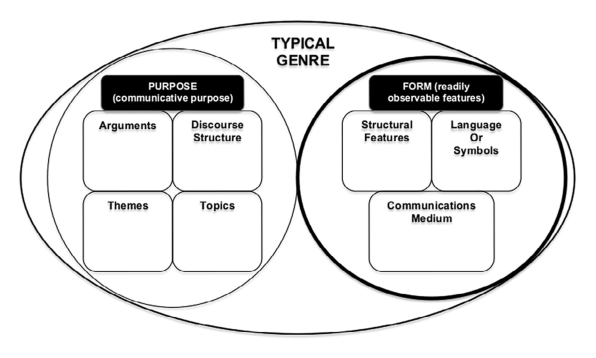
\includegraphics[scale=0.95]{Figures/Sotlen_diagram.eps}
		\caption{Stolen Imag.}
		\label{fiig:Stolen}
	\end{center}
\end{figure}







A very recent research on Cross-Lingual Genre Classification showed that it is possible to get very good results when an ML model is trained with a corpus samples of one language and then testing the trained model to an other. However, the evaluation framework was closed-set and the relation of the languages seems to be of a great importance for the accuracy performance of the model. That is, in some cases it was important the language to be of the same group for example the Roman or the Slavic group of languages and for others was not. Some times oddly the performance was dropping when the language was form the same language group \parencite{nguyen2019cross}.

Web Genre Identification (WGI) concerns the association of web pages with labels that correspond to their form, communicative purpose and style rather than their content. The ability to automatically recognize the genre of web documents can enhance modern information retrieval systems by enabling genre-based grouping/filtering of search results or building intuitive hierarchies of web page collections combining topic and genre information \parencite{Braslavski2007,Rosso2008,de2009genre}. For example, a search engine can provide its users with the option to define complex queries (e.g., blogs about machine learning or eshops about sports equipment) as well as the option to navigate through results based on genre labels (e.g. social media pages, web shops, discussion forum, blogs, etc). The recognition of web genre can also enhance the effectiveness of processing the content of web pages in information extraction applications. For example, given that a set of web pages has to be part-of-speech tagged, appropriate models can be applied to each web page according to their genre \parencite{Nooralahzadeh2014}. However, research in WGI is relatively limited due to fundamental difficulties emanating from the genre notion itself.


The most significant difficulties in the WGI domain are: (1) There is not a consensus on the exact definition of genre \parencite{crowston2011problems}; (2) There is not a common genre  palette that comprises all available genres and sub-genres \parencite{santini2011cross,mehler2010genres_on_web,mason2009n,sharoff2010web}, moreover, genres are evolving in time since new  genres are born or existing genres are modified \parencite{Boese2005}; (3) It is not clear whether a whole web page should belong to a genre or sections of the same web page can belong to  different genres \parencite{jebari2015combination,madjarov2015web}; (4) Style of documents is affected by both genre-related choices and author-related choices \parencite{petrenz2011stable,Sharroff2010}. As a result, it is hard to accurately distinguish between personal style characteristics and genre properties when style is quantified.

Genre means "genus" in the Greek language and for the text focused studies (either traditional linguistics or computational) mainly means style. The main utility of the genre taxonomy is for speeding up the communication in a broader sense. 

Starting with two cases outside the computer science the genre taxonomy is very useful in English 

One (REF) from the discipline of the \textit{English for Academic Purposes} (EAP) where it was vividly discussed the divergence in the genre taxonomies between the difference academic disciplines and reasoned the utility of the genre taxonomy for enabling the teachers and the students to improve their rhetorical and written language with the purpose of improving the teaching procedure. What is important to note for this study is the conclusion that the same genre-type can be very different for the communication purpose, i.e. as text identity carrier, but it can also contain the same style and other language properties when the purpose is similar, for example the article of new paper and an article form a magazine where one can claim that they are a different genre-type although they governed by the same linguistic properties.

The types of their study genre taxonomy mainly focused on the \textit{purpose} of the students written context and less on the \textit{style}, thus their genre-types where \textit{Creative Writing, Response Paper, Critique/Evaluation, Argumentative Essay, Report, Research Paper and Proposal}. Their study was a manual statistical process, similar to a \textit{Data Mining} process where grammatical features were counted in the texts. Then these features where indicating the score for each of the four (4) dimensions which has been qualitatively predefined. The counting process was using a heuristic computational tagger, named as Biber tagger (see Biber 1988 or ??? *** Genre variations in student .... (paper)).   
  
  ***
Genres, in textual sense, is sometimes defined as group of texts of documents that share a communicative purpose, as determined by the \textit{discourse community} which produces and/or reads them. "In \textbf{structural}terms, genre are social institutions that are produced, reproduced, reproduced or modified when \textit{human agents} draw on genre rules to engage in organizational communication".

"Layout in organizational communities cause people to focus perceptually on key parts of the text and our \textbf{empirical research has previously demonstrated that people use layouts and other related cues to focus on key parts of the text.}"
***


On the other hand and other research lying in the discipline of cognitive computing an health research they found humans are recognizing the genre type of a document or web-page using other cognitive processes relates mostly to the formatting of the text. Particularly they used as well configured apparatus for tracking the eyes movement while the recognition effort, where they fount that the eyes where following specific paths and where stopping to special landmarks on the text. They have concluded that the process of genre recognition was mostly related to the format and not the context, in addition they statistically measured that they previews experience was not related to the recognition process. Although it was the previews knowledge of the text formatting was accelerating the process. However, on the opinion of the authors of this study the genre recognition is a more deep process, thus as one can concluded by reading their study the landmarks they are referring into seems to be the only context combined with the formatting of the text that the human brain is requiring for identifying the genre-type. Given that their study is focused on the e-mail genres where formatting options compare to the web or textbooks is rather limited is advocating the conclusion that the minimum context is required for identifying the genre-type.

They are discussing of tree main perception (psychology) theories, i.e. Gestaltism (or Gestalt psychology), Ecological and Constructivism, which are the theories which can interpret the perception procedures, it this case the eye movement on the texts, to the cognition process for identifying the genre types of the texts. The perception procedure includes some eye movements mainly doing two tasks, \textit{scanning} and \textit{skimming}. Theses two procedures are irrespective of the belief of the supported interpretation theory related to the internal thought process for making a genre taxonomy decision. Scanning is the process where more or less we are trying to locate information of interest where the information has a homogeneous property, such as the a phone number in phone-book list. Skimming is the process where we are trying to locate information of interest where the information is raw or without a specific form, such as names, verbs, or phrases that is related to the abstract related concept in order to decide whether the text is matches and worth farther reading. 

The process of scanning and especially skimming in practice follows some specific eye movements, i.e. Fixation and Saccadic. Saccadic is the process while scanning or skimming that the eye is jumping around to the text, while Fixation is the process where the eye remains focused for a while. One can resemble the process like navigation where the eye is constantly moving while is focused for small fragments of time in landmarks of interest.
  
As \textit{Web Search} from an extension of IR because the main subject under investigation \parencite{manning2008introduction}, \textit{Web page Genre Classification } is becoming the main subject of document classification research.

Blogs is a genre-type has attracted as special interest on its own, in differed domains such as in sociology, psychology, linguistics and mostly in computational linguistics and WGI. There are several blogs' properties of interest of the research and  also blogs having their own sub-genre taxonomy. Blog-taxonomy general genres are \textit{Filter, Personal-diary} and \textit{Notebook} and other related to the authors group of styles such as \textit{Reflective, Narrative, Emotional, Rational} and \textit{Personal , Non-Personal}. The thought research on the blog-types classification has delivered a set of special linguistic and web-page structural properties which are increasing the performance of the closed set classification. Details for this linguistic properties used for specially for blogs sub-taxonomy classification are described in section \ref{chap:relevant_work:sec:features:subsec:heuristics} \parencite{virik2017blog,hoffmann2012cohesive,hoffmann2012cohesive,derczynski2014social,qu2006automated}. 

Most previous work in WGI follows a typical closed-set text categorization approach where, first, features are extracted from documents and, then, a classifier is built to distinguish between classes. Attention is paid to the appropriate definition of features that are able to capture genre characteristics and should not be affected by topic shifts or personal style choices. 

\section{Genre Definitions: The Linguistics and the Computational Linguistics}\label{chap:relevant_work:sec:definitions}

Overcoming the difficulties related to the genre taxonomy pointed out in linguistic and empirical studies, in text in \textit{text categorization} there is a great amount of work related to the automated categorization of texts based on \textit{genre taxonomy}. Although, starting from fundamentally different routes computational and linguistic studies, both ended up with the same notion of genre, which is eventually having two complimentary meanings,  i.e. \textit{Style} and \textit{Genus}\footnote{Genus in Greek means \textit{type} or \textit{class}} \parencite{sugiyanto2014term}. 

\paragraph{Definition Debate} In linguistic studies there is a great debate in defining \textit{the notion of genre} as an \textit{abstract categorization} of texts and the relation between them. Despite the methodological differences the linguistic community concluded that the idiosyncrasy of the \textit{genre taxonomy} is mutable and diverse \parencite{coutinho2009describe}. This kind of idiosyncrasy is yielded to the \textit{genre taxonomy} due to the spontaneous genesis of the genre classes. The genesis of a genre class is socio-centric interaction which is emerging from the need to describe the texts in order to accelerate the social communication procedure. Thus, genre classes are spontaneously emerging while the communication procedure is taking place.

\paragraph{Readers Perception} Humans can efficiently recognize the genre-types by processing the texts intuitively. However, there is a \textit{great luck of consensus} for the genre-types, particularly naming the genres. There there was an effort of several user studies for eliciting the mechanics in the process of \textit{genre identification and tagging}. The results on user agreement were very discouraging. Also, when it come to the reporting, i.e. for humans to describe specifically the terms or/and the attributes with which they use to identify the genre-types then there is a great confusion. A convincing reasoning for that is the plethora of textual, stylistic and conceptual terms which are used where they are different per individual and/or per group (e.g. teachers, scientists, engineers) for the same (or similar) text (or web-page) \parencite{roussinov2001genre, crowston2011problems}. 

Researchers, of cognitive computing and health research disciplines, found humans are recognizing the genre type of a document (or web-page) using other cognitive processes related mostly to the form of the text. Particularly they used as well configured apparatus for tracking the eyes movement while the recognition effort. One can resemble the process like navigation where the eyes are constantly moving while they are focusing for small fragments of time in landmarks of interest. The pausing of the eyes on the text "landmarks" is called \textit{Fixation} while the "jumping" movements of the eyes is called \textit{Saccadic}. The whole process was the effort to locate information of interest such as a specific text forms, names, verbs, or phrases that are related to the abstract concept in order to decide whether the text is matches and worth farther reading. They systematically found that the process of finding the genre-type of the text is the same as to find out whether a text worth farther reading. Thus, the genre taxonomy definitely accelerates the communication procedure and helping the reader of the text find the information of interest faster \parencite{clark2014you}.

\paragraph{Writers Awareness} In discipline of the \textit{English for Academic Purposes} (EAP)  it was vividly discussed the divergence in the genre taxonomies between the difference academic disciplines and reasoned the utility of the genre taxonomy for enabling the teachers and the students to improve their rhetorical and written language with the purpose of improving the teaching procedure. What is important to note for this study is the conclusion that the same genre-type can be vary differently form the communication purpose, i.e. as text identity carrier, but it can also contain the same style and other language properties when the purpose is similar, for example the article of new paper and an article form a magazine where one can claim that they are a different genre-type although they governed by the same linguistic properties. Therefore, for the witter of a text is is very important to be aware (thus to be taught) of the genre-type in order the text to be recognizable for the reader is seeking similar texts \parencite{hardy2016genre,melissourgou2017genre,al2017genre}.

\paragraph{"News" Sub-genres} The utility of the text genre identification (and/or classification) has been realized by the journalism historians. The technology advances and the new science innovations cased the attraction to the field. Journalism historians using a different genre-taxonomy where they mainly focusing on the purpose of the texts by analyzing the structure of the texts, where the structure consist of abstract elements. Their main genre-type are Inverted Pyramid, Martini Glass, Kabob, Narrative, Narrative and elements are \textit{Standard Lede, Body Section,  Narration, Synopsis, Image Lede}.  Similarly to the EAP domain, their sub-genre taxonomy is including genre-types like . \parencite{dai2018fine}.

\paragraph{Genre as Writing Style} The aforementioned variations of the genre taxonomy's notion is related more to the methodology and the objective of the text categorization task's specifications, rather than the philosophical difference. Particularly in author attribution domain there is a focus on identifying the \textit{style of the author} \parencite{stamatatos2009survey,koppel2011authorship,koppel2014determining}. On the other hand in the information retrieval (IR) domain, the interest is to classify the texts based on a predefined \textit{genre pallet}. Thus the interest is focused on the \textit{style of the authors group}, such as scientists, journalists, bloggers, etc.

\paragraph{The Web Genre} In consideration of \textit{the web genres taxonomy} it has been also eloquently analyzed the utilities and the difficulties for the web users. It has been pointed out that the genre taxonomy is summarizing the type and the style of the text in a single term as a communicative act [This conclusion cited also in \parencite{de2009genre}]. In the domain of \textit{web genre identification (WGI)}, \textit{the web genre taxonomy pallet} (which mostly used for research) has been formed in a top-down approach, where a group of experts are forming the taxonomy based on the specific objective of the task \parencite{crowston2011problems}. Moreover, in WGI research there was a very early observation that genre are organized in a hierarchical manner \parencite{wu2010fine}. Thus, most likely a web page might be multi-genre, the genre unit is considered to be the web-page \parencite{madjarov2015web,jebari2015combination}. However, in section \ref{} there is a discussion related the web-genre units other than the web-page.

As described so far, after a significant amount of work related to the study of the \textit{Genre-Taxonomy} and the \textit{Genre-Identification}, there is an agreement for the criteria which are defining the genres and the  web-genres. That is, the \textit{Form} and the \textit{Function/Purpose}. Complimentary criterion is the \textit{Context}, for example, the genre-type of the \textit{academic home web-pages} are easily identified by their context. The computational process of a text's \textit{context} is a standard procedure for the \textit{Topic Identification}. Although text's topic is considered as orthogonal to its genre, in cases such as academic home web-pages some context indicators can be exploited for the identification, also, of the Genre \parencite{coutinho2009describe,crowston2011problems,kanaris2009learning,jebari2015combination,gollapalli2011identifying}. 

Considering the above, it is clear that the Web-Genre Taxonomy has also a relatively abstract notion where is slightly changes depending on the research framework, despite the fact that the criteria for the genre-types of the texts are more or less common. Thus, for continuing the a this study in for the computationally, particularly NLP, research approach we are defining the notion of web-genre-type as follows.   

However, \textit{genre} itself requires different level of human reading abilities to be recognized and even with these skills different humans may disagree \parencite{mccarthy2009psychological}.

\begin{definition} Web-Genre-Type is defined as a class where its samples are i.i.d. Thus every web-unit (usually web-page) is always derived under a unique class distribution and the class distributions are not overlapped. That is, the Genre-Taxonomy consist from a distinctive non-overlapping classes/types.
\end{definition}

\section{Machine-Learning Methodology for Web Genre Identification and Classification}\label{chap:relevant_work:sec:machine_learning_methods}

In this work three algorithms are presented than can efficiently work on the WGI task in an open-set framework. There algorithms are inspired by some previews works on the AGI, which they have been adapted in fitting to the open-set classification requirements and to the \textit{web-genre noise} problem when it is assumed. In section \ref{chap:relevant_work:sec:openset_and_noise} these algorithms are discussed, together with other similar works towards to the open-set approach for WGI.

In this section it is summed up most of the machine learning models have been tested so far on the AGI (and especially the WGI) task. In addition, the most notable cases are presented in this section.

The main research volume have conducted experiments in a closed-set framework. The models have been commonly tested were the \textit{SVM, Naive Bayes, Random Forest, Decision Trees(C4.5), Ensemble based} models and the AdaBoost\parencite{lee2017text}. It seems that Random Forest and SVM were the top performing classification methods in the closed-set framework.

\paragraph{SVM Based} The SVM model was tested either in multi-class or binary form for the WGI \parencite{dai2018fine}. The model successfully been tested on \textit{Cross-Lingual Genre Classification} showed that it is possible to get very good results when an ML model is trained with a corpus samples of one language and then testing the trained model to an other \parencite{nguyen2019cross}. 

SVM also combined with several feature selection schemes, where most of them are presented in section \ref{chap:relevant_work:sec:features}. In \parencite{kanaris2009learning} is one of the first cases where the significance of the proper features for the SVM in WGI was pointed out. Specifically, the web-pages were projected in a feature space defined by a \textit{variable length Character n-gram corpus dictionary}. The dictionary composed from a mixture of size 3, 4 and 5 CNG features carefully selected from a modified version of the \textit{LocalMaxs }algorithm. The algorithm was using a \textit{"glue function"} for selecting the most informative n-grams and the rest of them where discarded.

\textit{Structure indicative features} have also been combined with SVM for the WGI task, specifically for the case of \textit{News article} sub-genre identification. Experimental results show that reasonable performance, although, this kind of features are importing even more issues. At first are difficulty to be captured for example counting the HTML tags or by analyzing the HTML DOM tree from a browser is the best practice to follow. Moreover, this kind of information usually is vague and small (Cortes and Vapnik, 1995) .

In \parencite{virik2017blog} SVM is compared with \textit{Naive Bayes Classifier (NBC)} and \textit{k-Nearest Neighbours kNN} on the classification accuracy for the \textit{Blogs' sub-genre taxonomy}. The results for the correlation of the \textit{linguistic features} and the \textit{Blog's sub-genres} shown that all three algorithms were successfully. However, SVM returned higher performance score. 

Although SVM algorithm is a high performance learner for the WGI task, it only can be competent for the closed-set classification framework. In the case of the open-set classification the performance drops significantly as shown in several studies (such as ...) and discussed later in chapter \ref{chap:openset}, where simpler \textit{Distance Based} methods seem to have higher performace.

\paragraph{Distance Based} There are several distance based approaches of the WGI task where it seems to have the highest performance in difficult cases such as the open-set WGI, and also when Noise is present. However, they have also been tested successfully in the closed set experimental setup.

One different case which is also bind to the feature selection is the \textit{Feature Difference Coefficient (FDC)} method. This method is based on the idea of the \textit{Ranked Features Distributions Distances} between the class-level features ranking and the document-level feature ranking. The features of the samples of a class are initially counted and their TF or TF-IDF values are ranked in a descending order. One can select the most frequent, but in the case study of \parencite{waltinger2010feature} the whole vocabulary have been used. Then a ranking sequential number is assigned and the frequency information is then discarded.

In order to compare a random web-page to the Class ranking the above procedure is repeated in the document level. Then for every feature present in the document and also present in the class vocabulary their ranking distance is calculated. The total sum or the distances is summed, while the norm value of the distances is assumed. Moreover, when a feature is not present in the document or the vocabulary then a Max value is assigned for this feature. The total ranking distance calculation is shown in equations \ref{eq:ranking_distance} and \ref{eq:ranking_distance_sum}.

\begin{equation}\label{eq:ranking_distance}
	d_{mnt} =
      \begin{cases}
      	| r_{mt} - r_{nt} |, t \in m \wedge t \in n  \\
        Max, t \notin m \vee t \notin n \\ 
       \end{cases}
\end{equation}
\begin{equation}\label{eq:ranking_distance_sum}
	IM_{mn}^{k} = \sum_{i=1}^{t} d_{mni}
\end{equation}
The smaller the $IM^{k}_{mn}$ total rank distance sums for all the $k$ feature the more is the similarity of the web-page pattern to the Class pattern. The features suggested (but not constrained) for this algorithm and for the WGI task are the following:

\begin{enumerate}
\item Word n-grams, Character n-grams, Word uni-grams and POS n-grams
\item Superficial and Structural such as the sentence length and the divisions number, and the paragraph length, concerning of the HTML text formatting.
\item HTML tag frequency in their logical structure, e.g. the number of <p></p> tags in total by ignoring the special cases of attributes or style sheets than might contain individually.
\item HTML Attribute Frequency same as in tags case.
\item First-Last tag frequency the x number of  the first occurring html tags and the y number of the last occurring tags.
\item Name entities frequency based on an entity recognition heuristic engine.
\end{enumerate}

In order to take into account all the above features contribution to the WGI task, a \textit{weighted sum all the} $IM^{k}_{mn}$ scores is calculated by the equation \ref{eq:ranking_distance_weighted_sumsum}

\begin{equation}\label{eq:ranking_distance_weighted_sumsum}
	C_{g} = \sum_{k=1}^{F} \delta_{k} \cdot IM_{mn}^{k}
\end{equation}
Where $C_{g}$ is the similarity score for the a genre of the taxonomy, and $\delta_{k}$ is the weight of the $k$ feature set from all $F$ features, where is under the constraint co $\sum_{k=1}^{F} \delta_{k} = 1$.

The accuracy using this method on shown to have been reached $93\%$ compare to $89\%$ of the SVM's performance, using the same features.


\paragraph{Neural Based} Recently Neural Networks have been used for modeling the WGI task (and other text classification tasks), additionally or independently of the Vocabulary modeling where neural-models have widely used. 

Most notably is the used of Recurrent Neural Networks (RNN) where Linguistic Complexity Contours (LCC) where employed as modeling features (LCC details are explained in section \ref{chap:relevant_work:sec:intro:subsec:heuristics}). Their model was based on 32 LLC features where fed to 32 Gated Recurrent Units (GRU)  and the output of each GRU was also fed to the next. Then all the output GRU output was the input of a Dense Layer of the RNN where a Softmax decision function was applied on. Their model was a closed-set framework with very high performance where was reaching over $90\%$  accuracy\parencite{strobel2018text}.

\paragraph{Ensemble Based} There are very few \textit{ensemble based} algorithms employed for the WGI and AGI task, however, they seem to be a very promising path as shown in \parencite{onan2018ensemble,pritsos2015clef,pritsos2013open,pritsos2018open}. Particularly there are three methods, mainly, where an ensemble can be formed, namely, AdaBoost, Bagging and Random Feature (RFS) Subspace ( (i.e. random sub-sampling). In this study we mainly focusing on the RFS, it is one of the algorithms are thoroughly presented in the context of WGI/AGI task.

\textit{AdaBoost} is a \textit{Boosting} algorithm where usually a random sampling is performed over the data and s set of classifier are trained over these samples. There is a weighting scheme over the samples which is changing in every training iteration, where for the samples mostly miss-classified, by most of the learners, their weights are increasing. In this manner the difficult samples repetitively to classification are presented to the weak learner in more iterations in order the whole systems of learners fit adjust better over these samples.

\textit{Bagging/Bootstrap aggregating} is an ensemble learning methods where a set of independent learners are training on different subsets of samples. Sampling with replacement is employed for Bagging, usually random. The performance of the ensemble is significantly influenced by the sampling policy/model. The ensembles decision is obtained either by the majority voting or my the weighted voting for a random sample.

Although, the traditional bag-of-words approach had better result with XABoost or other techniques been tested for over a decade on genre identification or/and particularly on WGI, distributional feature models are early showing their advantages over the TF-IDF (or TF alone) models[REF].

\textit{RFS } is mainly similar to Bagging in respect the sampling policy might be used. However, they deffer in the decision method where in RFS there is a \textit{$\kappa$ metric} or a \textit{$\sigma$ threshold} for the agreement of the weak learners for a random sample. This method also can be used for closed-set and open-set multi-class classification methods such as RFSE algorithms will be discussed in section \ref{}.

In \parencite{chen2012genre} an open-set ensemble presented where two multi-class SVM classifiers where trained for all the genres of their special formed genre-taxonomy for \textit{office documents} (details for office documents taxonomy find in \ref{}). Every SVM classifier was trained in a different mutually exclusive training subset, where the other part of the training set was used for tuning and vice-versa. The assumption of this training methods is that part of the support vectors  will be optimized for every SVM preserving the generalization of the two independent models and the combined classification will manage to fit well over the whole corpus. Their ensemble's decision rule as shown in equation \ref{eq:office_doc_ensemble} is a pairwise genre-class operation for an arbitrary page, where the truth table of this binary rule for all genre-class pairs might end up wilt all $0$ (zero) outcome. Then this page remains as unknown in all other cases at least one genre will return as true. On this combination rule several application can be operated as they have presented.

\begin{equation}\label{eq:office_doc_ensemble}
	(g^{k}_{1}[i] \vee g^{k}_{2}[i])  \wedge  (g^{m}_{1}[i] \vee g^{m}_{2}[i]) ,   \forall m \neq k
\end{equation}

where $\{k, m\}$ are the genre classes and $\{g_{1}, g_{2}\}$, are the genre SVM classifiers.
		
The above ensemble is an \textit{Early Fusion} category of ensembles where the potential different features and document representation are all combined in a sum-up vector for each document, i.e. a weighted sum or a concatenation of the different feature vectors. Then the summed-up vectors are the input for the learners of the ensemble where Bagging, Boosting, Majority voting or other strategies are used for then training and testing (or production) phases.

In \parencite{finn2006learning} a \textit{Late Fusion} ensemble is proposed for the AGI task which is an other category of ensembles. Late Fusion ensembles are composed from learners of the same model (say SVM, C4.5, NN etc) where every one is trained only on a specific feature set (or/and document representation). In the testing phase the ensemble me majority voting us a common strategy. 

Particularly the in their study they are testing C4.5 decision trees for BOW, POS, and \textit{Text Statistics} in detail explained in  section \ref{} they shown that their \textit{Multi View Ensemble }, i.e. the Late Fusion Ensemble, performs significantly better because every one of these features was a better choice only for a part of the genres in their taxonomy, thus the fusion of the all three increased the performance for all genre in total. In is important to note that in the training phase \textit{Active Learning}, and binary vector representation also were used. 

\textit{Active Learning} in their study was defined as a sample selection strategy while training where an an evaluating process was indicating which sample was better to be used for the specific C4.5 learner, for the specific features set. The Late Fusion ensemble with the active learning strategy shown to be a promising proposal for the Domain Transfer problem for AGI.

Additionally, other methods extending the ensembles methodology like Random Forests have been also became popular (see the following paragraph).

\paragraph\textbf{Domain transfer} is the ability to transfer across multiple-topic domains the same learner when it has been only trained in one of these domains. As an example, for the genre \textit{News} there might be several topic domains such as Sports, Technology, Science, Health, Politics. An ML model which has been trained for News only on Sports topic and still can perform similarly good for Technology, etc, it considered to perform well in domain transfer cases. This is very important particularly for AGI where usually the positive available sample for a genre are not available in a wide variate topic-domains (see section \ref{} discussing the genre taxonomy corpus building issues).

\paragraph{Domain transfer: Cross-Lingual Genre Classification} Similarly to the WGI domain transfer is the case of \textit{Cross-Lingual AGI} where the task is to train a model for classifying texts in a genre-taxonomy and on a \textit{specific mono-lingual corpus}. Then using the same trained model for classification to an other mono-lingual corpus but \textit{on a different language}, particularly with different linguistic properties such as English to Chinese transfer, and vice versa.

One proposed solution\parencite{petrenz2011stable}, is a combination of language independent features such as character-n-grams or/and superficial text characteristics such as \textit{Type/Token Ration} with an i\textit{iterative strategy of training a ML model}. Such a method is the \textit{Iterative Target Language Adaption (ITLA)}. 

\textit{ITLA} a special case of cross-lingual AGI method where pair-wise inter-language training is possible. That is, one can train a model to one language and then optimize it to an other. This method enabling the potential training of a model on one language and adapted to an other with very small labeled samples set for the required genre-taxonomy, but rich set of unlabeled samples. In \parencite{petrenz2011stable} SVM was the models of choice, The process includes the following steps:

\begin{enumerate}
\item Initially training an SVM classifier on language $L^{L}_{S}$. Then with the help of unlabeled $L^{U}_{T}$ set for the target language the model is \textit{evaluated for its prediction confidence} on the genre-taxonomy.
\item Using \textit{a labeled subset} of the \textit{target language set} $L^{L}_{T}$ an other SVM model is trained where the {prediction confidence} of the initial training is used for selecting only the samples of the subset returning the highest confidence score. 
\item The $L^{L}_{T}$  is clean by the samples with very low score and a new subset is re-sampled.
\item The process continues between the steps 2 and 3 until no change in the {prediction confidence} occurring or the iteration number has reached its max limit.
\end{enumerate}

An aspect is interesting to be mentioned is the set of features have been selected for training the above model. Mostly they are superficial, like Average Sentence Lenght and its STD, Average Paragraph length, Token-Type Ration, Numerical-Token Ration, Topic Average Precision, and a \textit{Single Line Sentence Ration and Distribution}. The Single Line feature refers to the cases where a paragraph of the text is just a single sentence where it seem to be a commonality to Reports, Official Documents and Academic documents.

The results in this study were very promising given that with a generic language independent approach manages to exceeds the results of the common solution of \textit{Machine Translation}. That is where the texts of the  source (where the model trained) of the target the language are translated automatically beforehand they are fed to the ML model.

\paragraph{Clustering Based and Hierarchical multi-class classification (HMC)} There a very special case, in \parencite{madjarov2015web}, worth to be motioned for the concept rather than its research value. Particularly is a primitive attempt to test the \textit{Hierarchical Multi-class Classification} on AGI. Although the results are relatively low in preforms and the experiments are not exactly comparable concerning the statistical consistency. However, there are several interesting aspects.

Firstly, they are using two \textit{clustering methods} attempting to develop an \textit{Automated Hierarchical Clustering (AHC)} where a raw multi-class taxonomy could potentially organized in a hierarchical manner. That is, given a set of  \textit{"leaf" class-tags} by using an agglomerative or a balanced k-means algorithm the tried to create a class-tag hierarchy and compare with the one of an expert. Secondly, they show than the Balanced k-means works better for this task on their data set and experimental set-up.

The utility of the Balanced K-means is for pre-defining the size of the clusters assumed to be. Thus, the objective function of the \textit{balanced k-means} is implicitly (or explicitly) optimizes two (contradictory) objectives. Firstly, is to find most dense and well separated clusters and secondly, is to maintain the sizes of the clusters equal. To do so, the \textit{Hungarian algorithm} algorithm is used for the optimization process \parencite{malinen2014balanced}, where it is a combinatorial optimization algorithm that solves the assignment problem in polynomial time.

Their method compared with the hierarchical taxonomy created by an expert, seems to work equally or betters for the HMC scenario of AGI. They also show the their result of the AHC can be also used for  a multi-class classification scenario.

\paragraph{Random Forest} Several studies among other classification algorithm they have extensively used \textit{Random Forest Classifiers}. Usually they use this algorithm in an out-of-the-box format. Most importantly seem to be one of the high score performance algorithms and most of the time the best solution. Although, most the studies are focusing of features selection/extraction and the term weighting schemes one could reason the high performance of the Random Forests to its internal ability to selecting the internal connection of the  features which \textit{resembles the word embedding} (FIND REF FOR THIS ARGUMENT) \parencite{sugiyanto2014term}

\paragraph{Semi-supervised classification (Co-Training} In section \ref{corpus_building} the genre-taxonomy corpus building task is discussed, where it is pointed out the issues of insufficient number of characteristic examples related to the positive samples for the genres of a taxonomy. Moreover, in section \ref{noise} the noise is discussed and the lack of negative samples in the available research corpora. These issues are labor intensive and very hard to be resolved even with the attempt of the cowed sourcing engines (like \textit{Amazon Mechanical Turk}) as presented in \parencite{Asheghi's relative work}. 

However, there might be an other path to follow when one would like to focus fore the classification aspect of the WGI, rather than the genre taxonomy itself. One suggested path is the \textit{Semi-supervised classification} in order to exploit the virtually infinite number of \textit{unlabeled}, in respect of genre, web-pages of the Web. Particularly in \parencite{chetry2011web}\textit{ Co-Training} is suggested for SVM and Naive Bayes classifiers with a set of $20000$ unlabeled samples in addition to the 1232 labeled web-pages.

The Co-Training is based on an iterative process where the unlabeled data are classified by the initially trained classifier. In every iteration the highest ranked unlabeled samples, in terms of classification certainty of the classifier, are fed to the re-training process to the classifier together with the previously labeled samples. The process continues until all unlabeled samples have been used or a specific number of interaction is reached. 

A significant improvement found where the ROC AUC score reached $0.730$ compare the supervised classification with score $0.713$ for SVM. The experiments where set on a closed-set framework with a corpus including the genes of \textit{Spam, Discussion, Educational Research, News Editorial, Commercial, Personal Leisure}.

Concerning the classification models involved in WGI studies, when a given genre taxonomy is utilized and there is no noise, then well-known machine learning models, like SVMs, decision trees, neural networks, naive Bayes, Random Forests, etc. are used \parencite{Lim2005,santini2007automatic,kanaris2009learning,jebari2015combination,sharoff2010web}. 

In case of presence of  noise, in a clustering framework described in \parencite{kennedy2005automatic} one cluster is built for each predefined class and another cluster is built for the noise. However, the most  common approach to handle noise is to build binary classifiers where the positive class is based on a certain predefined category and the negative class is based on the concatenation of  all other predefined categories plus the noise \parencite{kennedy2005automatic,dong2006binary,levering2008using}. Such a combination of binary classifiers can also be seen as a multi-label and open-set classification model where a web page can belong to different genres and it is possible for one page not to belong to any of the predefined genres. More concrete open-set  classification models for WGI were presented in \parencite{stubbe2007genre,pritsos2013open}. However, these models were only tested in noise-free corpora \parencite{pritsos2015clef}. More  recently, Asheghi \parencite{Asheghi2015} showed that it is much more challenging to perform WGI in the noisy web in comparison to noise-free corpora.

In section \ref{chap:relevant_work:sec:openset_and_noise} the open-set approach for WGI when noise is present, or not.

\section{Web Genre Noise and the Open-set approach}\label{chap:relevant_work:sec:openset_and_noise}

The main contribution of this work is the establishment of the novel open-set approach for the WGI and AGI tasks. In addition three previously presented algorithms adapted to the open-set classification and they are also presented briefly in this section together with an only few other similar efforts to towards to this research direction. The algorithms are thoroughly presented and evaluated in the following chapter \ref{chap:openset}, while in chapter \ref{chap:noise} are stressfully tested under the presence of noise.

Most previous studies in WGI consider the case where all web pages should belong to a predefined taxonomy of genres \parencite{Lim2005,santini2007automatic,kanaris2009learning,jebari2014pure_URL}. Putting this setup under the vantage point of machine learning, it is the same as assuming what is known as a closed-set problem definition. However, this naïve assumption is not appropriate for most applications related to WGI as it is not possible to construct a universal genre palette a priori nor force web pages to always fall into any of the predefined genre labels. Such web pages are considered \textit{noise} and include web documents where multiple genres co-exist \parencite{santini2011cross,levering2008using}. 

To handle noise in WGI there are two options. First, to adopt the closed-set classification setup having one predefined category devoted to noise. Since this category would comprise all web pages not belonging to the known genre labels, it would not be homogeneous. Moreover, this noise class would be much more greater with respect to the other genres causing class imbalance problems. 

The second option is to adopt the open-set classification setting where it is possible for some web pages not to be classified into any of the predefined genre categories \parencite{pritsos2013open,pritsos2015clef,pritsos2018open}. This setup avoids the problem of class imbalance caused by numerous noisy pages and also avoids the problem of handling a diverse and highly heterogeneous class. On the other hand, open-set classification requires strong generalization with respect to the closed-set setup \parencite{scheirer2013toward} and showed that it is much more challenging to perform WGI \parencite{Asheghi2015}.

The effect of noise in WGI  was first studied in \parencite{shepherd2004cybergenre,kennedy2005automatic,dong2006binary,levering2008using} where predefined genres were personal, organizational, and corporate home pages \textit{while noise consisted of non-home pages}. However, the distribution of pages into these four categories was practically balanced, hence it was not realistic.

\textit{Noise} in WGI can be categorized into \textit{Structured Noise (s-noise)} and into \textit{Unstructured Noise (u-noise)}, where s-noise defines as the collection of web pages belonging to several (known) genres. However, it is highly unlikely that such a collection  represents the real distribution of pages on the web. On the other hand, u-noise defines a random collection of web-pages \parencite{santini2011cross}.

There are few studies where they have handled somehow the \textit{structured and unstructured noise} in a closed-set approach. That is either the "noise" was assumed in the training phase of the prediction model where some sample had been left as \textit{outages} \parencite{jebari2015combination}, or s-noise has been used \textit{as a negative class} for training a binary classifier \parencite{Vidulin2007}. Noise also\textit{ used as the majority class} in experiments where one class was the positive sample case and several other genre with combination of some other randomly selected pages where used for fitting prediction models binary or multi-class \parencite{dong2006binary,levering2008using}. 

Open-set classification models for WGI were first described in \parencite{pritsos2013open,stubbe2007genre}. These models were tested in \textit{noise-free} and \textit{noise-full} corpora \parencite{pritsos2015clef,pritsos2018open,pritsos2019open}. Particularly, these are the models are described in detail in section \ref{chap:openset} and they are the main contribution to the domains of WGI and AGI. Here, are briefly described.

Recently, \textit{Ensemble Methods} were shown to achieve high effectiveness in open-set WGI setups \parencite{pritsos2013open,pritsos2015clef,pritsos2018open,pritsos2019open}. Two variants are studied in detail in this work, where one is based on the OC-SVM or $\nu$-SVM and the other is based a random features sub-sampling distance comparisons called \textit{RFSE (Random Feature Subspace Ensemble)}. 

One-class SVM is actually an $\nu$-SVM for the case we want to find the contour which is prescribing the positive samples of the training set given for a single class, while there are \textit{no negative samples}. $\nu$-SVM is providing an alternative \textit{trade-off control method of misclassification}, proposed from Scholkopf et al. \parencitep{scholkopf1999estimating}. 

It should be noted than $\nu$-SVM has the $\nu$ parameter which is regulating the following properties of the algorithm.
\begin{itemize}
\item $\nu$ is an upper bound on the fraction of \textit{Outliers}.
\item $\nu$ is a lower bound on the fraction of \textit{Support Vectors}.
\end{itemize}

In practice different values of $\nu$ are defining different proportion of the training sample as outliers. For example in Scholkopf et al. \parencitep{scholkopf1999estimating} is showed that in their experiments when using $\nu=0.05$, 1.4\% of the training set has been classified as outliers while using $\nu=0.5$, 47.4\% is classified as outliers and 51.2\% is kept as SVs.

In the prediction phase in order for an OCSVM model to decide whether a document is belonging to the target genre-class (or not) a \textit{decision function} is used. The decision function indicates the distance of the document, positive or negative, to the hyperplane separating the classes. In the case of OCSVM we are usually only interested whether the decision function is positive or negative for deciding if an arbitrary document belonging or not to the target class.

The ensemble form of  OCSVM proposed in this work, and published in \parencitep{pritsos2013open}, is described in algorithm \ref{alg:OCSVM-Ensemble}. Specifically, an OCSVM is trained for every web-genre class individually. In the prediction phase, the document is assigned to the class with the highest positive distance from the hyperplane (or the contour for OCSVM). If all OCSVMs return a negative distance (i.e. the web-page does not belong to this genre) the document remains unclassified, that is the final answer corresponds to "I Don't Know". Note than the $\nu$ parameter is the same for all the OCSVM learner. 

The RFSE algorithm is a variation of the method presented in \parencitep{koppel2011authorship}. In this work the RFSE shown in \textit{Algorithm \ref{alg:RFS-Ensemble}}. There are multiple training examples (documents) for each available genre from which a \textit{centroid vector} is calcualted for each genre. In the training phase, a centroid vector is formed, for every class, by averaging all the Term-Frequency (TF) vectors of the training examples of web pages for each genre.

An random document is compared against every centroid and this process is repeated $I$ times. Every time \textit{a Different Feature Sub-set is used}. Then, the scores are ranked from highest to lowest and the number of times the document is top-matched is measured, with every class. The \textit{document is assigned to the genre with maximum number of matches}. A $\sigma$ threshold is regulating amount of documents remaining unclassified, i.e. the RFSE responds "I Don't Know" for these documents.

The similarities function which they have been tested was cosine similarity, MinMax similarity, its combination. The similarities are combined in a way where their confidence scores are compared among all iterations at the end of the process for every document. Moreover, cosine and MinMax have different mean and standard deviation for the set of all evaluation documents and all iterations per document, thus the scores are first normalized and then are combined to amplify the confides score towards the dominant prediction.

An other recent approach related to the open-set classification on the \textit{Text Classification} problem was suggesting the reduction of the \textit{open space risk} using an SVM based methodology. Particularly, they are comparing eight (8) SVM based methods (additionally with an EM Semi-supervised method) in a open-set setup. They have compared their method with an  SVM center-based similarity space learning methods and some other methods, also in a open-set setup. Their method outperformed the others significantly, with some exceptions. 

Their main contribution is the transitions of the problem form the \textit{feature space} to the \textit{distance space}. Particularly they are using ten (10) different centroids one for each of the five (5) different distance measures proposed by (Fei and Liu 2015......) and for two (2) different document representations one for uni-grams and one for bi-grams. Their centroids are calculated using  eq \ref{eq:manning_centroids} 

\begin{equation}\label{eq:manning_centroids}
	c_{j} = \frac{\alpha}{\lvert D_{+} \rvert} \sum_{d_{i} \in D_{+}} \frac{x_{j}^{i}}{\lVert x_{j}^{i} \rVert } - \frac{\beta}{\lvert D - D_{+} \rvert} \sum_{d_{j} \in D - D_{+}} \frac{x_{i}^{j}}{\lVert x_{i}^{j} \rVert}
\end{equation}

where $D_{+}$ is the set of documents in the positive class and $\lvert . \rvert$ is the size of function. $\alpha$ and $\beta$ are parameters, which are usually set empirically.

The SVM methods under testing where 1-vs-rest multi-class SVM (Platt200...), 1-vs-set Machine SVM \parencite{scheirer2013toward}, W-SVM (Scheirer2014....), $P_{1}$-SVM (Jain2014), $P_{1}$-SVM (Jain2014), Exploratory Seeded K-means (Exploratory EM) (Dalvi2013...). They have also used a kind of \textit{openness testing}, by using $25\%$ to $100\%$ of the classes and their method were mostly outperforming the other methods. The macro-F1 score range of their methods from the most open set-up to the totally closed (i.e. using the $100\%$ of the classes) was from $0.417$ to $0.873$ depending on the corpus and the special class set-up \parencite{fei2016breaking}.

In this work it is presented an adapted implantation, for the WGI task, of the \textit{Nearest Neighbours Distance Ration (NNDR)} which it is also handles the open space risk and it is presented in detail in chapter \ref{chap:openset} and described in algorithm \ref{chap:openset:alg:NNDR_fitting}.

NNRD algorithm is our variant implementation of the proposed in \parencite{mendesjunior2016}. In the original approach euclidean distance has been used because of the variation of data set on which the algorithm has been evaluated. in algorithm \ref{chap:openset:alg:NNDR_fitting}, the cosine distance is used, because in text classification is being confirmed to be the proper choice in hundreds of publications. 

The NNRD algorithm is an extension of the \textit{Nearest Neighbors} NN algorithm where additionally to the sets of training vectors (one set for each class) a threshold is selected by maximizing the \textit{Normalized Accuracy} (NA) as shown in equation\ref{eq:NA}) on the \textit{Known} and the \textit{Marked as Unknown samples}.

\begin{equation} \label{eq:NA}
    NA = \lambda A_{KS} + (1 - \lambda) A_{MUS}
\end{equation}

\noindent
where $A_{KS}$ is the \textit{Known Samples Accuracy} and $A_{MUS}$ is the \textit{Marked as Unknown Samples Accuracy}. The balance parameters \lambda regulates the mistakes trade-off on the known and marked-unknown samples prediction.

The optimally selected threshold is the the \textit{Distance Ratio Threshold} (DRT) where NA is maximized. Equation \ref{eq:DR} is used for calculating the Distance Ratio (DR) of the two nearest class samples, say $s_{c_{a}}$ and $u_{c_{b}}$, to a random sample $r_{x}$ under the constrain $c_{a} \neq c_{b}$, where $c_{g}$ is the sample's class.

It is very important to note that the $c_{g}$ is trained in an open-set framework, therefore, the samples pairs selected for comparison might either be from the known of the marked as unknown samples. Thus $g \in {1,2,...,N}$ and $g = \emptyset$ when samples is marked as unknown.

\begin{equation} \label{eq:DR}
    DR = \frac{D(r_{x}, s_{c_{a}})}{D(r_{x}, s_{c_{b}})}
\end{equation}
\noindent
where $D(x,y)$ is the distance between the samples where in this study is the \textit{Cosine Distance}.

Therefore, the fitting function of the NN algorithm, described in algorithm \ref{chap:openset:alg:NNDR_fitting}, is the optimization procedure to find the DRT values for classes respective sets of training samples where NA is maximized.

The NNDR is a open-set classification algorithm, therefore, a random sample will be classified to one of the classes it has been trained or to the \textit{unknown class} when its DR score is greater than DRT threshold. During training the DRT values are tested incrementally until the optimal data are fitted for the training function.

In prediction phase the DRT is passed to the NNDR prediction function together with the training samples as shown in algorithm. Then for every sample of the testing set a classification decision is returned as shown in algorithm \ref{chap:openset:alg:NNDR_prediction}.

To sum up, as concerns the classification models involved in WGI studies, when a given genre taxonomy is utilized and there is no noise, then well-known machine learning models, like SVMs, decision trees, neural networks, naive Bayes, Random Forests, etc. are used \parencite{Lim2005,santini2007automatic,kanaris2009learning,jebari2015combination,sharoff2010web}. In case of presence of noise, in a clustering framework described in \parencite{kennedy2005automatic} one cluster is built for each predefined class and another cluster is built for the noise. However, the most common approach to handle noise is to build binary classifiers where the positive class is based on a certain predefined category and the negative class is based on the concatenation of all other predefined categories plus the noise \parencite{kennedy2005automatic,dong2006binary,levering2008using}. Such a combination of binary classifiers can also be seen as a multi-label and open-set classification model where a web page can belong to different genres and it is possible for one page not to belong to any of the predefined genres. 

More concrete open-set classification models for WGI have been presented here are the RFSE and the NNRD . In the  next chapters these algorithms together with the issues related to the model building for the WGI task in an open-set framework with the presence of Noise is analysed in details. Before that there is one more issue one could pursue in this research domain however it out of the scope of this work and that is way is only preseted here briefly in subsection \ref{chap:relevant_work:sec:temporal_wgi}

\subsection{Web Genre Temporal Property}
\label{chap:relevant_work:sec:temporal_wgi}
The temporal idiosyncrasy of the genre-taxonomy is a major factor, yet not deeply studied in the linguistics and computational linguistic domains. Naturally, as in other human arts there is an evolution in the genres, while other genres emerging and others stop existing. Web-genre taxonomy is a result of an even more dynamic environment and it evolves rapidly. Genres are adapting due to the medium transition such as from \textit{News on paper} to \textit{News on the Web}, or because of the medium itself emerging novelties such as the \textit{Blogs} which have evolved to\textit{ micro-Blogs} and finally to \textit{the Social-Media}. 

In \parencite{caple2017genre} there is a characteristic study advocating in the temporal manner of the web-genre, where it is analyzed how the News (as a web-genre) have changed overtime and the way the News sub-genres occurred.

An \textit{Enhanced Centroid-based Classification (ECC)} ensemble model has been proposed for dealing with adapted genres and the temporal idiosyncrasy of the genre-taxonomy. The model is an \textit{incremental centroid-based} ensemble where new web pages are classified one by one, where in the testing/production phase the centroids adjust to the new data as long as they are "close-enough" \parencite{jebari2015combination}.

The ECC learning algorithm is calculating an initial set of centroids for every given class based on the equation \ref{eq:jebary_ecc_centroids} and then using the threshold calculated by the equation \ref{eq:jebary_ecc_theshold} is re-evaluating the samples. When the samples of  class are not "close-enough" are considered to be \textit{outages} and a new centroid is calculated from the rest of the samples for this class. 

\begin{equation}\label{eq:jebary_ecc_centroids}
	GC_{i}^{N} = \frac{GC^{S}_{i}}{\Vert GC^{S}_{i}\Vert }
\end{equation}

\begin{equation}\label{eq:jebary_ecc_theshold}
	\sigma_{i} = \frac{1}{\vert g_{i} \vert } \sum_{p_{j} \in T_{r_{g_{i}}}} sim(p_{j}, GC_{i}^{N})
\end{equation}
\noindent
where $GC^{S}_{i} \in G$ is a set of predefined genre centroids for the $S_{i} \in G$ set of samples for each genre class $G$. $T_{r_{g_{i}}} =   \{ (p_{i}, g_{j}) \vert g_{i} \in G  \}$ is a set of training set samples initially and at the and is formed to $T_{r_{g_{i}}} =   \{ (p_{i}, g_{j}) \vert sim(p_{j}, GC^{N}_{i}) \leq \sigma_{i} \}$  after eq. will be applied \ref{eq:jebary_ecc_theshold}.

In the testing phase an arbitrary page is ranked in deciding order to the \textit{similarity-rank} $\theta(p)$, as defined in the equation \ref{eq:jebary_ecc_rank}. Then the centroids and the threshold are re-calculated based on the equations \ref{eq:jebary_ecc_new_centr} and \ref{eq:jebary_ecc_new_thres}. 

\begin{equation}\label{eq:jebary_ecc_rank}
	\theta_{i} = \{g_{i}, sim(p, GC_{i}^{N}) > \sigma_{i}\}
\end{equation}
\begin{equation}\label{eq:jebary_ecc_new_centr}
	GC_{i}^{N} =  \frac{GC^{S}_{i} + p}{\Vert GC^{S}_{i}  + p\Vert}
\end{equation}

\begin{equation}\label{eq:jebary_ecc_new_thres}
	\sigma_{i} = \frac{S_{i} +  sim(p, GC_{i}^{N})}{\vert g_{i} \vert}
\end{equation}
The ECC has been \textit{designed to adapt in the evolution of genres in time}, thus, it makes no sense to classify the web pages exclusively on the contrary is returning the similarly-rank $\theta(p)$. Consequently, this algorithm can be considered open-set \textit{because possible for same web-pages the  $\theta(p)$ set might return empty}. On the other hand since the algorithm will adapt some web-pages that are not strictly belonging to the genre it is trained for, i.e. noise pages, will be incorporated to the new centroids and the threshold value.  Consequently, ECC is sensitive to noise as it has been defined in section \ref{chap:relevant_work:sec:openset_and_noise}.

\section{Features Selection and Vector Space Dimensions}\label{chap:relevant_work:sec:features}

In most of the applied research domains where machine learning is the dominant subject of choice the main concern is to extract and select the proper features from the raw data samples of the data set. Therefore, in addition to the process of inverting a machine learning method for inducing prediction models for the problem the process of feature extraction and dimensionality reduction are coming together. The same applies for the WGI where most of the focus where in these two procedures and less in creating new machine learning algorithms. On the contrary, in all studies usually a closed-set and out-of-the-box ML models were tested with the exception of the cases described in sections \ref{chap:relevant_work:sec:machine_learning_methods} and \ref{chap:relevant_work:sec:openset_and_noise}.

In this section are summarized all feature selection and dimentionality reduction successful ideas for WGI and AGI. To begin with the features that can be extracted from a web-pages can be grouped to the \textit{textual}, the \textit{HTML tags} and the \textit{URL links} with or without their \textit{anchor text}. Cornering the URL links it will be discussed in more detail in section \ref{chap:relevant_work:sec:url} where either the URL it self as a character string can be analyzed or the structure of the web-pages connections can be exploited \parencite{abramson2012_URL,asheghi2014semi,jebari2014pure_URL,priyatam2013don_URL,zhu2011enhance}. 

In respect of the HTML tags, the most adaptive approach it the frequency counting of the HTML tags distributed in the hypertext. Special focus in some cases are given to the image tags and the link tags\parencite{Lim2005,levering2008using}.  There are also other cases where only pure structural information of a web page, i.e. the HTML tags, are exploited {[}Philipp Scholl{]}. In addition there are very few cases where the DOM object structure is analyzed for extracting information but usually as part of the whole set of features selected and not as a stand alone choice \parencite{mehler2011integrating}.

The \textit{Textual content} is the most analyzed part of the hypertext which has been used for WGI \parencite{mason2009distance,Sharroff2010}. There are several features than can be extracted used alone or combined to getting the maximum information one can get from the web-paged and feed it for training a prediction ML algorithm. Character n-grams, Word n-grams, Part-of-Speach n-grams and some \textit{special discriminative words} have been commonly used and usually combined with some heuristically extracted features \parencite{kanaris2009learning,kumari2014web,levering2008using,Lim2005,mason2009n,onan2018ensemble,petrenz2011stable,sharoff2010web,Nooralahzadeh2014}.

The web-page's extracted features were also presented in a variety of  text  representation schemes such as Term Frequency (TF), Term Frequency  Inverted Document Frequency (TF-IDF), Binary Term, and Smoothing Distribution (see LOWBOW ref). The \textit{Superficial Document Characteristics (SDC)} can be considered as features and document representations together where they are the counts of the Words lenghs (in characters) frequency, the Sentencies length (in words) frequency, the Paragraphs length etc. In addition the Max, Min, and Ratios of these SDC were also count such as the \textit{Average to Max size of Words Ratio, the Max Word Length Frequency} etc. In general several facets, i.e. \textit{terms types}, have been tested for WGI cornering the Hypertext \parencite{feldman2009classifying,santini2005linguistic}.

 Superficial features, such as \textit{colon frequency, document length, sentence mean length and single-sentence paragraph count}, were successfully used as in input to an SVM classifier for a closed-set genre classification task where training and testing has been applied on different languages (cross-lingual genre classification) \parencite{nguyen2019cross}.

Usually, the combination of features from different sources enhances the robustness of WGI approaches \parencite{levering2008using,kanaris2009learning}. However, features extracted from textual content are more robust since they do not  depend on technology or format used to create a web page and therefore they are more likely to remain constant in time given that the W3C is changing the specification of the HTML regularly, for covering the occurring needs. This is the reason that this work is only focusing on the textual information in the next chapters.

Althought the textual information is more robust and constant in time there are a lot of heuristics that where successfully in WGI and AGI experiments. In section \ref{chap:relevant_work:sec:features:subsec:heuristics} the most interesting feature extraction heuristics are summarized.

\subsection{Heuristics has been used with success in WGI}\label{chap:relevant_work:sec:features:subsec:heuristics}

(ADD LOWBOW MAYBE)

Raw document pre-processing is essential part for the document categorization and this is the case for the WGI also. Several heuristic methods for selecting and/or extracting the document's information have been tested together with the representation of the extracted information a vector space. The objective o these heuristics is to capture the features carriers of the required information for training the model correctly and moreover, to reduce the vector space implicitly compare to the BOW approach.   

To begin with, it shown that the \textit{Writing Style Features} and \textit{Key Event Placement (KEP) Features} are improving significantly the performance of the SVM classifier \parencite{dai2018fine}.  The writing style features are extracted as a combination of  other complex features, i.e. the combination of \textit{grammar production rules (GPR} and features from a semantic category of a \textit{Linguistic Inquiry and Word count (LIWC)} dictionary. GPR are the combination of POS and word lexical rules. LIWC is a sophisticated dictionary of occurrences of word from a word category. The KEP is a set of text formatting features, or "landmarks", such as \textit{specific characters, time, location} at specific areas of the text. In practice it is the \textit{words overlapping count} between the \textit{first paragraph} and \textit{the title} of a document. The combination of these structured based features has improved the macro-F1 performance.

Another notable methodology in respect of the feature selection and document representation is the \textit{Complexity Measures (CM)}. Particularly a sliding window of characters and words is considered over a text. Then using this window several heuristics and superficial metrics are counted and/or calculated. Particularly there are 32 features, depicted in table \ref{chap:relevant_work:tbl:complexity_measures}. These features can be categorized in the following four (4) classes: (1) \textit{Raw Text Features} such as the Mean Sentence Length, (2) \textit{Lexical Features} such as Type Token Ration, (3) \textit{Morpho-Syntactic Features} such as Lexical Density, (4) \textit{Syntactic Features}, such as \textit{Complex Nominals} per term unit \parencite{strobel2018text}.

\begin{table}[t]
	\center
	\caption {Complexity Measures table as found in \parencite{strobel2018text}.}\label{chap:relevant_work:tbl:complexity_measures}
	\begin{tabular}{lll}
		\hline
		CM Name & Definition & NLP Category \\
		\hline
		Number of Different Words / Sample & $Nw_{diff} / Nw$ & Lexical \\
		Correct Type-Token Ration & $T/\sqrt{2N}$ & Lexical \\
		Number of Different Words & $Nw_{diff}$ & Lexical \\
		Root Type-Token Ration & $T/\sqrt{N}$ & Lexical \\
		Type-Token Ration & $T/N$ & Lexical \\
		Lexical Density & $N_{lex}/N$ & Morpho-Syntactic \\
		Mean Length Clause & $N_{W}/N_{C}$ & Morpho-Syntactic \\
		Mean Length Term-Unit & $N_{W}/N_{T}$ & Morpho-Syntactic \\
		Sequence Academic Formula List & $N_{seq}/AWL$ & Raw text \\
		Lexical Sophistication (ANC) & $N_{ANC}/N_{Lex}$ & Raw text \\
		Lexical Sophistication (BNC) & $N_{BNC}/N_{Lex}$ & Raw text \\
		Kolmogorov Deflate & KS2011 & Raw text \\
		Morphological Kolmogorov Deflate & KS2011 & Raw text \\
		Syntactic Kolmogorov Deflate & KS2011 & Raw text \\
		Mean Length Sentence & $N_{W}/N_{S}$ & Raw text \\
		Mean Length of Words & $N_{C}/N_{W}$ & Raw text \\
		Words on New Academic Word List & ${N_{W^{AWL}}}$ & Raw text \\
		Words not on General Service List & $\neg{N_{W^{GSL}}}$ & Raw text \\
		Clause per Sentence & $N_{C}/N_{T}$ & Syntactic \\
		Clause per Term-Unit & $N_{C}/N_{T}$ & Syntactic \\
		Complex Nominals per Clause & $N_{CN}/C$ & Syntactic \\
		Complex Nominals per Term Unit & $N_{CN}/N_{T}$ & Syntactic \\
		Complex Terms Units per Term Unit & $N_{CT}/N_{T}$ & Syntactic \\
		Coordinate Phrase per Clause & $N_{CP}/N_{C}$ & Syntactic \\
		Coordinate Phrase per Clause & $N_{CP}/N_{T}$ & Syntactic \\
		Dependent Clause per Clause & $N_{DC}/N_{C}$ & Syntactic \\
		Dependent Clause per Terms Unit & $N_{DC}/N_{T}$ & Syntactic \\
		Mean Length of Words (syllables) & $N_{Syl}/N_{W}$ & Syntactic \\
		Noun Phrase Post-modification (words) & $N_{NP^{Post}}$ & Syntactic \\
		Noun Phrase Pre-modification (words) & $N_{NP^{Pre}}$ & Syntactic \\
		Noun Phrase Pre-modification (words) & $N_{NP^{Pre}}$ & Syntactic \\
		Term Units per Sentence & $N_{T}/N_{S}$ & Syntactic \\
		Verb Phrase per Term Unit &  $N_{VP}/N_{T}$ & Syntactic \\
		\hline
	\end{tabular}
\end{table}

\textit{The Blog} is a genre with special interest for several research domains and as might be expected it has its own special set of heuristics for selecting informative features. This requires \textit{Lexical Analysis, Morphological Analysis, Lightweight Syntactical Analysis} and \textit{Structural Analysis}. In table \ref{chap:relevant_work:tbl:blogs_special_features} all the linguistic properties used for Blog's sub-genres classification are presented in detail. In \parencite{virik2017blog} there is a detailed analysis for the correlation of the \textit{linguistic features} and the Blog's sub-genres. Example of these sub-genre are \textit{informative, affecting, reflective, narrative, emotional} and \textit{rational}.

\begin{table}[t]
	\center
	\caption {Blogs' special features table as found in \parencite{virik2017blog}.}\label{chap:relevant_work:tbl:blogs_special_features}
	\begin{tabular}{p{4cm}p{7cm}p{3cm}}
		\hline
		Type & Description & NLP Category \\
		\hline
		Special Character Frequency & Frequency of: @, \#, \$, \%, <WhiteSpace>,\&, -, =, +, !,  ¿, ¡, [, ], /, | & Lexical \\
		Word Count & Number of alphanumeric tokens & Lexical \\
        Unique Lemma Count & Number of unique identified tokens & Lexical \\
        Abbreviation Frequency & Ration of abbreviations to all words & Lexical \\
        Ratio of long to short words & Long words consist of three and more syllables & Lexical \\
        Misspelled words Frequency & Ration of misspelled words of all words & Lexical\\
		Noun Frequency & Ration of nouns to all words & Morphological \\
        Adjective Frequency & Ration of adjectives to all words & Morphological \\
        Pronoun Frequency & Ration of pronouns to all words & Morphological \\
        Verb Frequency & Ration of verbs to all words & Morphological \\
        Proper Noun Frequency & Ration of proper nouns to all words & Morphological \\
        Ratio of Open to Closed words Classes & Words open to Inflection which include nouns, adjectives, pronouns, numerals, and verbs  & Morphological \\
        Ratio of functional to Content words Classes & Words with only grammatical function. Content words include nouns, adjectives, numerical, non-modal verbs and adverbs  & Morphological \\
        Frequency of sequences of functional words & Five of more consecutive functional words with tolerance of one closed word & Morphological \\
		Sentence Count & Number of identified sentences & Syntactical \\
        Average Sentence Count & Average sentence length in number of words & Syntactical \\
        Ratio of Simple to Compound Sentences & Compound consist of two or more sentences & Syntactical \\
        Average Sub-sentence Count & Sub-sentence is simple sentence inside a compound sentence & Syntactical \\
        Dominant Tense of  Predicted Candidates & Present, future and past & Syntactical \\
        Dominant Person of  Predicted Candidates & First, second and third & Syntactical \\
        Dominant Number of  Predicted Candidates & Singular and plural & Syntactical \\
		Link Frequency & Ration of number of Links to number of Sections  & Structural \\
        Image Frequency & Ration of number of Images to number of Sections  & Structural \\
        Section Count & Number of Sections & Structural \\
        Standard Deviation of Section length & Deviation of the number of words in sections & Structural \\
		\hline
	\end{tabular}
\end{table}

The \textit{automated genre-taxonomy} is a subject of interest in other domain of intellectual products (e.g. paintings, music, movies etc) as explained before. Movies taxonomy has also a special interest for the technology and entertainment industries, besides other methods a special interst for this work is the case where the genre of a moves is induced by textural features such as \textit{the subtitles} and the \textit{text description} of a video content. These features are summarized in table \ref{chap:relevant_work:tbl:videogenre_textbased_special_features}. Particularly, BOW, Superficial and Syntactical features were combined. Superficial features in this study were called \textit{content-free} and the ones related to specific words called \textit{content-specific} \parencite{lee2017text}. In the process it has been found that not all these features were so important. The most important of them were the \textit{Token-Type Ration, Words per minute, Characters per minute, Hapax legomena, Dis legomena, Short words ratio, Rations of  (10, 4, 3, 1)-letter words}. 

\begin{table}[t]
	\center
	\caption {Video content genre classification special features, based exclusively on text (subtitles etc) table as found in  \parencite{lee2017text}.}\label{chap:relevant_work:tbl:videogenre_textbased_special_features}
	\begin{tabular}{p{4cm}p{7cm}p{3cm}}
		\hline
		Type & Description & NLP Category \\
		\hline
		Average words per minute & & Textual/Superficial  \\
        Average characters per minute & & Textual/Superficial  \\
        Average word length & & Textual/Superficial  \\
        Average sentence length in terms of words & & Textual/Superficial  \\
        Type/token ratio & Ratio of different words to the total number of words & Textual/Superficial  \\
        Hapax legomena ratio & Ration of once-occurring words to the total number of words  & Textual/Superficial  \\
        Dis Legomena ratio & Ration of twice-occuring words to the total number of words  & Textual/Superficial  \\
        Short words ratio & Words less than 4 characters to the total number of words & Textual/Superficial  \\
        Long words ratio & Words more than 6 characters to the total number of words & Textual/Superficial  \\
        Words-length distribution & Ratio of words in length of 1-20 & Textual/Superficial  \\
        Function words ratio & Ratio of function words to the total number of words  & Textual/Superficial  \\
        Descriptive words to nominal words ratio & Adjectives and adverbs to the total number of nouns & Syntactical \\
        Personal pronouns ratio & Ratio of personal pronouns to the total number of words & Syntactical \\
        Question words ratio & Proportion of wh-determiners, wh-pronouns, and wh-adverbs to the total number of words & Syntactical \\
        Proportion of question marks to the total number of end sentence punctuation & & Syntactical \\
        Exclamation mark ratio & Proportion of exclamation marks to the total number of end sentence punctuation & Syntactical \\
        Part-of-speech tag n-grams & & Syntactical \\
        Word n-grams & Bag-of-words n-grams  & Textual/Content Specific \\
  		\hline
	\end{tabular}
\end{table}

Wikipedia and in general Wiki sites, is considered as a special genre due to its characteristic, mainly the rich of textual content per page and secondary its \textit{informative linguistic register}. Also there are several sub-genre wiki pages which are also characterized as \textit{Popular Science} web-site and web-documents (e.g. Wikipedia, Nature, New Scientist, Wikinews, etc). There are some heuristically selected features that seems to work well for classifying the wiki-pages into a sub-genre taxonomy. Table \ref{chap:relevant_work:tbl:pop_science_features} shows the set of features used for capturing sub-genre of the Popular Science. Testing these feature with a clustering algorithm it has been shown that 4 clusters can be formed with where their centroid have as significant distance. Thus the documents can be separated easily. Although, the performance scores were not very high this approach seems promising \parencite{lieungnapar2017genre}. 

\begin{table}[t]
	\center
	\caption {Popular science web-documents Sub-genres special features, based exclusively on text, found in \parencite{lieungnapar2017genre}.}\label{chap:relevant_work:tbl:pop_science_features}
	\begin{tabular}{p{2cm}p{12cm}}
		\hline
		Type & Description \\
		\hline
		Average sentence length & Average number of words per sentence with the text. Longer sentences are commonly used to mark complex and elaborated structure. \\
        \hline
        Average paragraph length & Average number of sentences per paragraph with the text. Longer paragraphs are frequently used to mark information density. \\
        \hline
        Discipline-specific word density & Number of specialized vocabulary items in content-specific areas as a proportion of total number of words. Discipline-specific words are frequently used to express referential information in specific subject areas. \\
        \hline
        Phrasal verb density & Number of phrasal verbs as a proportion of total number of verbs. Since phrasal verbs manifest a degree of informality and textual spokenness, a high frequency of this feature suggests a narrative purpose. \\
        \hline
        Compound noun density & Number of open compound nouns as proportion of total number of nouns. A high frequency of compound nouns indicates greater density of information. \\
        \hline
        Modal verb density & Number of modal verbs as proportion of total number of words. Modality is used to mark explicit persuasion.  \\
        \hline
        Verb density &  Verbs indicate a verbal style that can be considered interactive or involved and are used for overt expression of attitudes, thoughts, and emotions. \\
        \hline
        Adjective density & Number of adjectives as proportion of total number of words. A high frequency of adjectives can be associated with high informative focus and careful integration of information in a text. \\
        \hline
        Adverb density & Number of adverbs as a proportion of total number of words. Adverbs are used more frequently to indicate situation-dependent reference for narrating a story. \\
        \hline
        Lexical repetition & Yule's characteristic K, the variance of the mean number of occurrences per word. The larger Yule's K, the more the lexical repetition, Greater use of repetition results from the purpose of explicitly marking cohesion in a text and informative focus.  \\
        \hline
        Coordinating conjugation density & Number of coordinating conjunctions as a proportion of total number of sentences. Coordinating conjugations are commonly used to show formality in reverentially explicit discourse.  \\
        \hline
        Content word density & Number of content words as proportion of total number of words. Content words mark precise lexical choice resulting in presentation of informative content.\\
        \hline
        Evaluation move density & Numbers of evaluation moves as portion of total number or sentences. Evaluative language in normally used to express emotions and attitudes.  \\
        \hline
        Vocabulary diversity & Sums of probabilities of encountering each word type in 35-50 tokens. A high diversity of vocabulary results from the use of many different vocabulary items. Narrative texts often have high vocabulary diversity.  \\
        \hline
        Logical connective density & Number of logical connectives per 1000 words. A high frequency of logical connectives indicates an informative relation in a text.  \\
        \hline
        Prepositional phrase density & Number of prepositional phrase per 1000 words. Prepositional phrase indicates a greater density of information.  \\
        \hline
        Negation density & Number of negation markers per 1000 words. Negation is preferred in literary narrative.  \\
        \hline
        Pronoun density & Number of pronouns refer directly to the addressor and addressee and thus are used frequently in highly interactive discourse. \\
        \hline
        Flesch Reading Ease & Flesh Reading Ease formula. Higher Flesch reading scores are easier to read.  \\
  		\hline
	\end{tabular}
\end{table}

\textit{Registers and Genres} are correlated and also used interchangeably, although different. A set of \textit{ "abstract" features} can be used for explicitly correlating \textit{the registers} and the \textit{Popular Science sub-genres}.  In table \ref{chap:relevant_work:tbl:pop_science_registers_features} are presented these abstract features are listed, which potentially can be tested for any \textit{register to genre} correlation other than the aforementioned use case.

\begin{table}[t]
	\center
	\caption {Popular science web-documents Sub-genres registers to features correlation, found in \parencite{lieungnapar2017genre}.}\label{chap:relevant_work:tbl:pop_science_registers_features}
	\begin{tabular}{p{4cm}p{7cm}p{3cm}}
		\hline
		Pop Science Sub-Genre & Key features & Text-Registers \\
		\hline
		 Sub-genre 1 & Phrasal verb density, verb density, adverb density, vocabulary diversity, logical connective density, negation density, pronoun density, Flesch reading ease & Interpersonal, Narrative, Persuasive, Informative \\
         Sub-genre 2 & Modal verb density, Flesch reading ease & Interpersonal, Persuasive \\
         Sub-genre 3 & Average paragraph length, Lexical repetition, Evaluation move density, Prepositional phrase density & Informative\\
         Sub-genre 4 & Average sentence length, Discipline-specific word density, compound noun density, adjective density, coordinating g7conjunction density, content word density & Informative, Elaborated, Impersonal  \\
  		\hline
	\end{tabular}
\end{table}

As registers are also considered as genres then there is also a set of heuristics have been used for a classification for this taxonomy. Particularly in \parencite{onan2018ensemble} Language Function Analysis (LFA) has been introduced for a classification task on a taxonomy of \textit{Expressive, Appellative,} and \textit{Informative} classes.

The LFA is combining features that successfully used for Authorship Attribution (AA), Linguistic Features (LF), Character n-grams (CNG), Part of Speech n-grams (POSNG), and the frequency of the most discriminative words (MDW). 

\begin{itemize}
\item Features used in authorship attribution (AA) usually are words, POS n-grams, character n-grams, capitalized words, lowercase words frequency, punctuation and quotation marks frequencies. 
\item Linguistic features (LF) usually are time and money entities, POS, personal pronouns, possessive pronouns, adjectives and nouns frequencies. 
\item Character n-grams (CNG) usually means their frequency of the n-grams, over a specific frequency threshold, say at least 4 times occurrence. 
\item Part of speech n-grams (POSNG) same as CNG but for POS.
\item The frequency of the most discriminative words (MDW) this is usually task dependent.
\end{itemize}

\textit{News} sub-genres is also a subject of great interest in several domain related to text categorization. The News sub-genre are also resembles more to document registers such as the case of $\{News-Fact, News-Opinion, Review-Positive, Review-Negative\}$. This kind of classification is also called {Domain Transfer} AGI Task \parencite{finn2006learning}. 

\textit{Text Statistics} features have been used for such a task described in table \ref{chap:relevant_work:tbl:domain_trans_text_statistics}. It seems that special function words frequencies have a special significance in these special case. 

\begin{table}[t]
	\center
	\caption {Text Statistics, found in \parencite{finn2006learning}.}\label{chap:relevant_work:tbl:domain_trans_text_statistics}
	\begin{tabular}{p{3cm}|p{11cm}}
		\hline
		Feature Type & Features\\
		\hline
		 Document Superficial Statistics & Sentence length, Number of words, Words length \\
         Frequency of various function words & because, been, being, beneath, can, can’t, certainly, completely, could, couldn’t, did, didn’t, do, does, doesn’t, doing, don’t, done, downstairs, each, early, enormously, entirely, every, extremely, few, fully, furthermore, greatly, had, hadn’t, has, hasn’t, haven’t, having, he, her, herself, highly, him, himself, his, how, however, intensely, is, isn’t, it, its, itself, large, little, many, may, me, might, mighten, mine, mostly, much, musn’t, must, my, nearly, our, perfectly, probably, several, shall, she, should, shouldn’t, since, some, strongly, that, their, them, themselves, therefore, these, they, this, thoroughly, those, tonight, totally, us, utterly, very, was, wasn’t, we, were, weren’t, what, whatever, when, whenever, where, wherever, whether, which, whichever, while, who, whoever, whom, whomever, whose, why, will, won’t, would, wouldn’t, you, your \\
         Frequency counts of various punctuation symbols  & ! " \$ \% ' ( ) * + - . : ; = ? \\
  		\hline
	\end{tabular}
\end{table}

\paragraph{Image processing features for document AGI} In \parencite{chen2012genre} there is a very interesting approach where image processing features have been used for the AGI for categorizing \textit{office documents}. In their experiments interestingly the image-based features were significantly better that the text-features when coopering their work to previews ones. The combination of both was increasing the performance even more.

The image-based features were extracted by splitting the image of the document into 25 tils (5 horizontally and 5 vertically) plus a full-page til. The image-based features used where; (a) \textit{Image Density}, (b) \textit{Horizontal projection}, (c) \textit{Vertical projection}, (d) \textit{Color Correlogram}, (e) \textit{Lines}, (f) \textit{Image Size}. In all cases the documents images where converted to back and white for these features to be extracted. The exception is the \textit{Correlogram} which is analyzing the full color spectrum of the document's in its image format.

\begin{itemize}
\item The \textit{Image Density} utility was used for differentiating where the images and the text was located. In addition the titles form the rest of the text could be also separated. To capture this feature the black to total pixels ration was calculated for each til of the document. 
\item The \textit{Horizontal Projection} was used for differentiating the slides where the text is large and less than the rest of the non-slides documents. After the process required for locating the text boxes (similarly tho the OCR software) then a five-bin histogram were used for identifying the majority of the text font sizes.
\item The \textit{Vertical Projection} was used to differentiating the papers from tables by capturing the number of text columns and the distribution of their width. Similarly to the horizontal projection a five-bin histogram of column width were used.
\item The \textit{Color Correlogram} is representing the spatial correlation of colors. The process is starting by quantizing the colors to a 96 scale in distance range for 0 to 1. In addition 3 pixels are used thus every til of the document has 288 dimensions. The selection of the optimal features for reducing even farther the dimensions was operated using Maximally Relevant Minimally Redundant (mRMR) method, resulting 50 features pare til. The preservation of the location of the spatial color correlation coefficients is important thus an implicit strategy was followed. Particularly after the mRMR the selected features where preserved to their til-vector position and then all tils vectors concatenated into one vector. Finally the non-selected features from mRMR where discarded and the "compressed" form of the concatenated vector was the final outcome of the Correlogram preprocessing.
\item The \textit{Lines} was used particularly for locating tables. The process was operated on the full-page til and it was measuring the continues sequence of black pixels of the black and white form of the picture. Then a line-length histogram was used for discriminating the table lines from other lines present in a text such as header of footer lines often met in textbooks.
\item The \textit{Image Size} was operated only on the full-page size, for finding the page size of the document and differentiate the papers form slides or picture usually having different sized while papers usually delivered in a specific size page size.
\end{itemize}

However, their experiments where conducted to a very special case of  the AGI research and for a very specialized taxonomy the \textit{office documents}. The corpus was including \textit{Papers} such as PDF, \textit{Photos} such as JPG, \textit{Slides} such as PowerPoint, \textit{Tables} in documents. This corpus has been collected manually and then also manually annotated. \textit{Fleiss' Kappa} agreement score for the annotators, has been used in order to evaluate the quality of their corpus (the \textit{Kappa} score was from 0.88 to 0.92).

The image-based features described above are similar to the ones used from the human evaluator in \parencite{clark2014you} described in \ref{chap:relevant_work:sec:linguistics_definition}.

\paragraph{Graph based features} Several heuristics, superficial, lexical, grammatical, syntactical and specialized to context information has been explored for WGI/AGI in the context of using the textual information of the text/web-pages. However, there is a effort from \parencite{nabhan2016graph} where they using Graph-based features for \textit{Text Genre Analysis}. This work is no testing these features for identification or classification. However, it seems that the texts-genres are having \textit{Graph Properties Measurements} than can potentially could be used for automated identification.

The graph measures has been analysed related to the text-genre were \textit{Node degree, Clustering Coefficient, Average Shortest Path Length, Network Diameter, Number of Connected Components, Average Neighborhood Connectivity, Network Centralization} and \textit{Network Heterogeneity}. The graph they used was constructed be Word 2-Grams (bigrams). The graph was underweight and no bigram frequency was considered.  

The average node degree, i.e. the number of neighbors connections, shown  to be a discriminating criterion for discriminating for example \textit{scientific} to \textit{humor genres}. Higher average node degree may indicate a preference to use established vocabulary than a random one.

The clustering coefficient with high value would mean there is tendency for a set of nodes to cohere or stay connected in a sub-network. The \textit{Religion, Fiction} and \textit{Adventure} seems to have higher value to their clustering coefficient compare to \textit{News, Editorial} and \textit{Hobbies}. 

The Number of connected components with high number is indicating a \textit{Topic Diversity} within genre. News and Hobbies shown to have higher score, i.e. higher diversity, than Religion and Fiction. Related to this, also high score in Network Centralization seems to be a good indicator for Fiction and Adnventure genres.

The Network Heterogeneity where shown to be higher in News and Hobbies reflects the tendency of the graph to have alto of links between high-degree to low degree-nodes. This can indicate tendency to use functional keywords in text.

\textit{Genre-specific graph characteristics} also found it this study. Such as, \textit{high global clustering coefficient} found for Learned and Religious text genres. Moreover, the \textit{Average Local Clustering} strongly correlated to the node degree shown to be a good indicator for genres showing concentration to \textit{specific concepts}.

Ultimately, the graph-metric patterns can also be used for discovering the existence of sub-genre within a genre such as in News. It has been shown that there are some areas in the News genre bigram graph with \textit{High Node Connection Concentration (or High edge Concentration}.  

\paragrpah{Readability Assessment Features} Finally, the \textit{Readability Assessment Features (RAF)} have also been tested for the WGI/AGI task. Moreover, a primitive attempt also presented related to these features where they have been evaluated (and compared to others features) in their effectiveness on different taxonomies. Particularly they compared on the \textit{Domain-taxonomy} and the \textit{Genre-taxonomy} \parencite{falkenjack2016exploratory}.

Although, there is a ambiguity in the research literature related to the Domain/Genre definition, usually the genre considers to be (as explained in section \ref{chap:relevant_work:sec:definitions}) more abstract and related to \textit{the texts organization, rhetorical structure, length, syntax, morphology} and \textit{vocabulary richness}. Domain is more related to the \textit{General topic of a group of text}. Consequently, \textit{Sports} as category is considered to be a Domain while \textit{Academic papers} are considered Genres.

It has been shown that genre-taxonomy ML classification is benefit by the use of RAF while the domain-taxonomy does not. 

The RAF are very old in because they are studied since 1920 where their main purpose is to help in the evaluation of a text in respect the ease in reading and comperhation by the abilities of the reader. Although, the function includes two (2) variables the research is mainly focusing on the aspect of the evaluation of the text side only. 

The most basic metrics are LIX metric (see eq \ref{chap:relevant_work:eq:LIX}) , OVIX (Word Variation Index) and NR (Nominal Ration) metric. However, since the evolution of ML there are several other text information have been evaluated and also used in combination with the basic metrics \parencite{falkenjack2013features}.

RAF other than the basics are including some \textit{Superficial features, Lexical features, Morpho-syntactic features} and \textit{Syntactic features}. Specifically the selected features from every lingustic categories are:

\begin{enumerate}
\item Superficial: Average Word Lengh (in Characters), Averga Word Length Syllables per word, Average Sentence Length.
\item Lexical: Vocabulary Lemmas for Communication, Everyday use, High frequent, Unique.
\item Morpho-syntactic: Unigram-POS, Ration-to-content of nouns, verbs etc.
\item Syntactic: Average Dependency Distance, Ration of Dependencies, Sentence Depth (in dependency terms), Unigram Dependency Type (based on token terms), Verbal Roots, Average Verbal Arity, Unigram Verbal Arity, Tokens per clause, Average Nominal Pre and Pos Modifiers, Average Number of Prepositional components.
\end{enumerate}

It should be noted that other than the basic LIX, NR and the Superficial of the RAF, all the other are language dependent such as the OVIX which mainly has been tested on Swedish language.

\begin{equation} \label{chap:relevant_work:eq:LIX}
	LIX = \frac{A}{B} + \frac{C \cdot 100}{A}
\end{equation}
Where $A$ is the number of words, $B$ is the number of periods (colon, dot, capital fist letter), $C$ is the number of long words, more than 6 letters for the English language. 

\subsection{Feature Selection and Term Weighting Schemes}
 
 \textit{Term Weighting Schemes} is also an essential issue together with the features selection for the pre-processing of the web-pages and the induction of the ML models for WGI task.

 \paragraph{TF-IGF}  The \textit{term weighting schemes} is an other aspect have been considered merely for WGI. Most of the studies were commonly selecting the  TF-IDF schema. In the study of \parencite{sugiyanto2014term} it is shown that TF-IDF is not the proper schema for the WGI task. On the contrary a TF-IGF schema was proposed and shown to perform better. 
 
TF-IDF is a balancing weighting scheme of the document's terms (Word n-gram, Character n-gram, POS n-gram, etc), in a collection of documents, where it regulates the information value of the very low and very high frequency terms of the collection. That is, it decreases the value of the very high frequency terms, and increases the the very low frequency terms when they are occurring in a high amount of documents in the collection ( and also  low in the document level). The calculation of a terms IDF in a documents collection is shown in equation \ref{chap:relevant_work:eq:idf}
 
 \begin{equation}\label{chap:relevant_work:eq:idf}
 	IDF(T) = log \left( \frac{N}{1 - f_{D,T}} \right)
 \end{equation}
\noindent
where $N$ is the number of the collection documents and $f_{d,t}$ is the \textit{frequency of the documents} where term $t$ occurs. Following the same line of thought, and replacing the collection of documents with a \textit{collection of documents on a specific genre} TF-IGF is a weighting schema where the high frequency terms in the genre are smoothed and the low frequency terms are weight higher as long as they occur in a significant amount of documents of this genre. Then in a multi-genre corpus the \textit{Term Frequency - Inverse Genre Frequency (TF-IGF)} is calculated as in equation \ref{chap:relevant_work:eq:tf_igf}

 \begin{equation}\label{chap:relevant_work:eq:tf_igf}
 	F^{TF-IDF}(T) = f_{T,G_{i}} \cdot log \left( \frac{N}{1 - f_{G_{i},T}} \right)
 \end{equation}
\noindent
where $f_{T,G_{i}}$ is the frequency of the Term in the genre and $F^{TF-IDF}(T)$  is the TF-IGF. In  \parencite{sugiyanto2014term} they also used the average $Avg(F^{TF-IDF}(T))$ for ranking the terms and they have tested the 100, 500, and 1000 most frequent in average terms. Comparing them with the averaged TF-IDF on their 7-Genre corpus they show clearly that the confusion matrix has great improvement when it used as an input to a \textit{Random Forest Algorithm}. Especially for the 100 features where the $F_{1}$ climbed from $0.091$ to $0.642$ and for 500 to $0.775$ from $0.249$.

Although the improvement was impressive by just changing the weighting schema, especially for  the size of the vector space, one should consider that the experimental set-up was only for the closed-set scenario. Moreover, the TF-IGF similarly to the TF-IDF is tightly related to the collection itself, therefore, the results closely are related to the 7-Genres collection. Given that these collection are old and the nature of the highly temporal idiosyncrasy of the genre-taxonomies, it is high likely this method to have high bias. On the other hand in closed-set cases where the texts collection is constrained considering documents number (i.e. slowly expanding) and genre-taxonomy size (i.e. rarely updated) the TF-IGF seems to be efficient, and with very low computational cost.  

\textbf{Fuzzy extension of TF-IDF} In section \ref{chap:relevant_work:sec:features:subsec:heuristics} a set of heuristics presented where Video content can be categorized on its respective genre taxonomy based on the textual information of the videos such as the subtitles and the small description of the video. In formation from public site like IMDB and Movelens. There it is also possible for the the users to create their own \textit{tags} in addition to the \textit{keywords} mainly created for the data curators of these sites. 

These user created tags can be exploited in a similar manner as the words of the subtitle text for classification of the video to their genre. Particularly there is a work where the \textit{tags}, and the \textit{keywords} are used for multi-class classification task of Movies upon their genre. It has been shown that the user tags is a rich information source and more effective than keywords alone. However, the user tags wouldn't be useful features without the proposed \textit{Fuzzy extension of TF-IDF weighting schema}.  This schema returned $F_{1}$ score up to $0.9$ when user tags alone where used.

Although the above method was aiming for building an effective recommendation system here it is presented briefly for the innovative weighting scheme which is exploiting the meta-data of the tags. Particularly the aforementioned user tags are in fact triplets of  $\{Tag, Movie, User \}$. The idea is to exploit the frequency of the users selecting a tag for a movie and then the frequency of the movies a tag was occurring, similarly to the TF-IDF.

To do so initially the \textit{Appropriateness} of a tag is evaluated by counting the number of time a user is tagging a movie with the same tag when a movie is belonging to a specific genre by using equation \ref{chap:relevant_work:eq:fuzzy_movies_genre_eq1}

\begin{equation}\label{chap:relevant_work:eq:fuzzy_movies_genre_eq1}
	tf_(u_{j},g_{i}) = \frac{\sum_{m \in G} tagged(t,u,m) }{ \max_{t \in T} \sum_{m \in G} tagged(t,u,m)}
\end{equation}
where $tagged(t,u,m)$ is 1 when a user $u$ tag with t the movie $m$ when it belongs to genre $g$, and $0$ if not. The score of a tag similar to the TF-IDF is called Degree $deg(t,m,g_{i})$and it is the weighted frequency of users as singed this tag by the \textit{Importance Score} $imp(t,g_{i})$ of the tag, as shown in equation \ref{chap:relevant_work:eq:fuzzy_movies_genre_eq2}

\begin{equation}\label{chap:relevant_work:eq:fuzzy_movies_genre_eq2}
	deg(t,m,g_{i}) = uf(t,m) \cdot imp(t,g_{i})
\end{equation}
Where $uf(t,m)$ is the frequency of the users assigned the this tag to a movie $m$. The $imp()$ is calculated by the \textit{Fussy Linguistic Ordered Weighted Averaging Aggregation Operator (OWA)} of the equation \ref{chap:relevant_work:eq:fuzzy_movies_genre_eq1} weighted by the \textit{Uniqueness} of the tag. The uniqueness is also the OWA compliment of the term among all the genres of the taxonomy. The $imp()$ is then calculated by the equations \ref{chap:relevant_work:eq:fuzzy_movies_genre_eq4} and \ref{chap:relevant_work:eq:fuzzy_movies_genre_eq4}.

\begin{equation}\label{chap:relevant_work:eq:fuzzy_movies_genre_eq3}
	t_{most}(g_{i}) = \oint_{j=1}^{U} tf_(u_{j},g_{i})
\end{equation}

\begin{equation}\label{chap:relevant_work:eq:fuzzy_movies_genre_eq4}
	imp(t,g_{i}) = \oint_{j=1}^{U} tf_(u_{j},g_{i}) \cdot (1 -  \oint_{i=1}^{G} t_{most}(g_{i}))
\end{equation}

Where $\oint=OWA$,  $g_{i}$ is a particular genre, $G$ is the number of the genres in the taxonomy and $U$ is the number of users used this tag for this genre.

Finally, for the movie genre categorization a binary vector of the genres list is returned of the \textit{Quantised  $\max_{t \in T} deg()$}. The maximum degree values of the genre tag is set to $1$ when it is above the \textit{mean values of all tag-degrees} and zero otherwise.

\section{Dimensionality Reduction}

Dimentionality reduction and the \textit{selected features encoding in to a multi-dimensional vector} is an important aspect concerns the WGI research. As aforementioned \textit{features selection} implicitly affects the compression of the vector space, however, there are other explicit methods than have been tested for WGI.

BOT and TF-IDF approaches seems to work almost as good as more complex features such as POS, $\chi^{2}$ statisics etc. However, in some cases explained before such as Wikipedia, blogs, news sub-genre the complex features (and heuristics) seems to work better. It seems that is is the result of the implicit dimentionality reduction which enables an ML model to be optimized in a more informative vector space.

Although, the above statement might be a subject of a great research arguments, what we unsuitably know is that in a smaller and more informational dense vector space a ML algorithm will perform much better with great certainty. Thus, a method that could potentially reduce the vector space and manage to encode the maximum of the required information, it would at least improve significantly the speed performance of any ML algorithm. 

In order to make an intuition about the "curse of dimensionality"  and on how the feature selection can encode more information in case dimensionality reduction, a mind experiment is presented bellow. 

Lets assume task where a ML model should be trained in a multi-class classification task for the whole genre-taxonomy of the WWW and assuming that all the genre of the Web where idd and known. In that case the whole Oxford Dictionary would have defining the vector space of the problem. 

The Oxford dictionary English is containing $171,476$ words thus the vector space would have been very sparse. The amount words can be calculated also by using the Combinatorial Calculation using the \textit{binomial coefficient} minus the invalid combinations, of the $26$ English letters (assuming the the whole Web was only written in English language), as shown in equation \ref{chap:relevant_work:eq:en_vocab_size_calc}.

\begin{equation}\label{chap:relevant_work:eq:en_vocab_size_calc}
	 \left(
    	\begin{array}{c}
        	n = 26\\
            k = 1\\
         \end{array}
	\right)
    +
    \left(
    	\begin{array}{c}
        	n = 26\\
            k = 2\\
         \end{array}
	\right) 
    +
     \cdots 
    +
   \left(
    	\begin{array}{c}
        	n = 26\\
            k = Max Eng. Word\\
         \end{array}
	\right) 
    = 300,430 - \{Invalid Combinat.\} =  171,476
\end{equation}
On the other hand if we are using the Character n-grams of size $3$ (C3G) or $4$ (C4G) then for C3G the vector space is $2600$ \textit{minus the set of invalid combinations} and for C4G becomes $14950$. As we also know from the literature and it will presented later in this study the CNG features are returning the highest score in WGI ML modeling. Moreover, the \textit{character tuples} are capturing stylistic properties of the texts, where it is an information which is lost when it is "hidden" in the words.

To conclude, dimentionality reduction is the main objective in the process of feature selection and as explained so far there are several heuristics than can applied to achieve this. There cases where a terms (word or char, n-gram) is selected only when it can be counted in more than a specific number of web-pages in a corpus. Moreover, there are cases where only the words above a specific threshold are selected, usually the length varies from 2 to 5 characters length. In addition is has been shown that \textit{Stop words} (Stamatatos) and 
\textit{Surface cues} (Kessler) from the superficial document metrics are important and some time better (and lighter in terms of speed in model training) than the raw BOT. 

All the aforementioned approaches is a implicit method for dimentionality reduction and documents information encoding. However, \textit{Graph based features} is an explicit method for this and usually is applied after them feature selection process.

\textit{Distributional Features/Word Emending} based on the words or/and document encoding is the state-of-the-art in IR and NLP because it a practical solution for automatically modeling the process of feature selection, document representation and dimentionality reduction. This is the case for the AGI/ WGI tasks, and it is the second contribution to the domain together with the open-set approach.

In section \ref{chap:Document_Representation} and it is shown how a week ML algorithm can be trained with 100 times less features than the features given to an better algorithm for the WGI task. Moreover in section \ref{chap:relevant_work:sec:word_embedding} there is a discussion related to the word embedding and the \textit{Features Vocabulary Modeling}.

%\section{Web-Genres Identification using other than textual information}\label{chap:relevant_work:sec:intro}

\section{Deep Learning Vocabulary of Distributional Features for WGI}\label{chap:relevant_work:sec:word_embedding}

Given the complicated task of AGI, the traditional BOW models are unable to capture the enduring information span across sentences and paragraphs. Themes, registers and other properties of the texts cannot be captured only by the frequencies of the Terms (Word, Character, POS n-grams etc). The abstract concepts, the ontologies, the style and the form of the texts are only merely captured by a combination of heuristics as explained in section \ref{chap:relative_work:sec:heuristics}. 

The feature selection is so important that so far the simpler the model the better performs for the WGI task as long as the features are capturing \textit{the style and the concepts} of the texts. In \parencite{pritsos2019open}, which is part of this work, and also in \parencite{worsham2018genre} the \textit{Neural Language Modeling (NLM)} is proposed for the first time for WGI an AGI respectively. In both works the conclusion is similar. i.e. the ensemble based and boosting methods which are rather simpler than NLM are stile better performers on the task. However, in respect of speed performance and the automation in the process of feature selection the NLM seem to be the perspective research path for the following years.

Most proposed \textit{NLM} are designed to capture text in a sequential manner. That is, the model is encoding the meaning of the words based on the sequence of the previews terms (or following terms). Therefore, these models also called \textit{Distributional Models (DM)} and the NLM process is also called \textit{Word Emending}. The NNet models which have been tested are the \textit{Convolutional Neural Networks (CNN)}, the Recurrent Neural Networks (RNN), and the \textit{Long Short-Term Memory Networks (LSTM)}. 

The experimental procedures of this work is confirming the speed amplification in the WGI training and prediction process, mainly due to the dimentionality reduction and the better encoding of the abstract information required. However, it is also confirming that the process more the NLM was computationally expensive because of the length of the texts. In \parencite{worsham2018genre} there was an effort to reduce the problem and increase the performance of the NNet models.

Working with long pieces of text the NNet for example CNN the network is increasing as the data input is growing. On the other hand the RNN and the LSTM are sensitive to long sequences and their hyper-parameters are degenerated then they are becoming very slow in training for overcoming this issue. Moreover, to train these NNet models with long corpora is required a great hardware infrastructure. 

In order to reduce the training time and computational cost of the word-embedding modeling one can think of several strategies. It turns out that the best strategies is to use the \textit{All Chapters} training input. That is,  the training and the test set is splinted into chapters in a heuristic manner. Then the lengths of the chapters are normalized by getting only the $C_{Doc}$ length of the whole chapter, say the first 2,000 terms. In case the chapter is shorter the rest of the chapter is padded with an abstract term such as $\$pad\$$. 

As it has been reported the all-chapters strategy with a CNN returned $F_{1}=0761$ score which was the best of all the NNet combinations and features sizes. However, \textit{Random Forests} or \textit{XGBoost on sequential trees} and simple BOW, outperformed the NNet model with $F_{1}=0.79$ and $F_{1}=0.81$ respectively. XGBoost is a highly optimized, \textit{Gradient Boosting }solution which is made up of a boosted set of sequential trees learned from the gradients of some differentiable loss function\textbf{ (Chen and Guestrin, 2016).}

In \parencite{pritsos2019open} a work is presented where Doc2Vec has been used for the WGI task on KI04 corpus. Detail are discussed in section \ref{word_embedding}. It is shown that \textit{Distributional (DL) features} can make a weak open-set learning algorithm namely the \textit{Nearest Neighbour Distance Ration} classifier to a combative learner. When it come to comparison in the open-set framework with the RFSE, the NNDR seems performing lower, however, the size of the document vectors are 10 to 100 times smaller because of the DL features. 

In these experiments the whole KI04 corpus is given to the NNet document encoder. The line of thought is the same as Word2Vec and the word embedding, i.e. as an extension of the words encoding the documents can be encoded to a fixed size vector space. 


% ""Examples of word vectors include Word2Vec (Mikolov et al. 2013), GloVe (Pennington, Socher, and Manning 2014), Eigenwords (Dhillon, Foster,and Ungar 2015), and Fasttext (Bojanowski et al. 2017). These word vectors are usually referred to as distributional word vectors, as their training methods rely on the distributional hypothesis of semantics (Firth 1957)."""


The state-of-the-art in the text-genre classification and WGI is the Vocabulary-Learning and particularly the use of the deep-learning methods for building comprehensive word encoding vocabularies or document encoding. 

This methods due to the nature of the Neural-Networks, mainly used,  the procedure for building vocabulary models is \textit{implicitly embedding} a variate of information\textit{ syntactical, morphological and structural}. However, there are some efforts, where these kind of information was \textit{"explicitly encoded"} by using other methods inspired by signal processing and dimentionality or noise reduction techniques.


In \parencite{kim2010formulating} it is proposed the \textit{Harmonic Descriptor Representation (HDR)} of the web-pages inspired by the musical analogy of a string musical instrument. Then the document is consider to be a temporla sequence of signals, i.e. the characters or word n-grams. In similar manner to the NLE models it is captured explicitly the \textit{Distributional Properties} of the texts. Particularly instead of the terms occurrence counting the intervals of the the occurrences are measured, in addition the length of the documents are encoded and normalized implicitly. 

The HDR word encoding is a tuple of three explicit measurements; the FP, LP and AP. Moreover the \textit{Range} and the \textit{Period} are also introduced. The \textit{Range} is the interval between the initial an the ultimate occurrence of the term and the \textit{Period} is the "time duration", i.e. the count of terms, between two conductive occurrences of the term. Therefore, the HDR vectors components are defined as follows:

\begin{enumerate}
\item FP: is the time duration before the first occurrence of the term in a web-page. That is the Period before the first occurrence divided by the total number of terms into the page.
\item LP: is the time duration after the last occurrence of the term. Similarly calculated as FP.
\item AP: is the average period ration as in equation \ref{chap:relevant_work:sec:word_embendding}.
\end{enumerate}

\begin{equation}\label{chap:relevant_work:sec:word_embendding}
	AP  =
      \begin{cases}
        \frac{N - T}{T \cdot I^{max}}, I^{max} > 0  \\
        1, I^{max} = 0 \\ 
       \end{cases}
\end{equation}

\noindent
where $T$ is the term's number of occurrences plus $1$, $N$ id the total number of pages terms and $I^{max}$is the maximum number of characters found between two consecutive occurrences of the term. The more harmonic the distribution of a terms in a documents the more the $AP$ is closer to $1$.

The HDR vocabulary modeling in the \textit{7-Web} genres corpus managed to return a accuracy score $0.96$ with the SVM algorithm in a closed set classification experimental setup.

Alternative methods and similar the HDR is the \textit{Pointwize Mutual Information (PMI)}. It is the Post-processing of the resulting modeled vectors. Such example is the \textit{unsupervised Post-processing via Conceptors (or Conceptor Negation)}. The main concept is to suppress the outages frequencies using PCA, SVD and most recently Conceptors Negation. The latest is a methodology (unsupervised) of Conceptors are a family of regularized identity maps introduced by (Jaeger 2014 ???) where a linear transformation is taking place minimizing a loss function similar to the PCA process. However, this methodology on the contrary to the PCA is a "Soft" regularization or "Soft" noise filtering, while PCA is considered "Hard". In both cases by projecting the data-point to the prediction space we are able to filter the noise (or outages) samples (CITE Unsupervised Post-processing of Word Vectors via Conceptor Negation ).

Textual feature selection and document representation is the main research focus for WGI, with the NLM being the most promising path to follow for the near future. However, the URL and the Hypertext linking graph are the properties of the web-pages have also been exploited in the WGI research.  Analogous to the surface and structural types of cues for text features, these features can be treated as cues for extending or mining additional information for the classification process. In addition, some time for example in the cases of the very short textual information in a web-page, the URL and the sibling (in graph) pages are necessary for correctly identifying its genre. 

In section \ref{chap:relevant_work:sec:url} the URL and the hypertext graph linking is discussed before the open-set and the NLE modeling, for WGI, will be thoroughly analyzed as the main focus of this work.

\section{The Hyper (URL) links significance}\label{chap:relevant_work:sec:url}

In the IR research, related to the Web-Site/Page search result ranking the URL as a hyperlink and as a string describing the source location is essential element. This is the case also for the WGI task, where both properties of the URL have been tested. In this section all of the effort where the URL have been used substantially and not just as part of the BOW approach are described. 

The URL elements exploitation is out of the scope of this work because this work is focusing on the exploitation on the textual information, its encoding, and the ML algorithms for this purpose. On the contrary the URL is changing the definition of the web-genre unit from the web-page to different variation such as the web-site or the section of a web-page. On the whole, the URL for WGI can be consider an amplifier mechanism for the signal than an ML algorithm is using for fitting a model for WGI.

To begin with, a study is based on the web-graph and the implicit genre relation among web pages assuming that neighbouring web pages are more likely to belong to the same genre, a property called \textit{homophily}. Then, the content of neighboring pages is used to enhance the representation of a given web page in a semi-supervised learning framework \parencite{asheghi2014semi}...(More details to be written here)

\textit{GenreSim} is a link-based graph model which exploits \textit{link structure} to select relevant neighbouring pages in order to amplify the information required for a page to be classified to a genre taxonomy. This algorithm is improving significantly cases where the textual information is very low in a web-page such as a web page such as Movie Homepages, Photography websites etc. Particularly in their experiments GenreSim ((( compare to RFSE was performing significantly grater in their \textit{genre-taxonomy corpus named IV-12} with such idiosyncrasy (i.e. move homepages, photography etc) and less or no improvement on corpora such as 7-Genre or KI-04 \parencite{zhu2011enhance,zhu2016exploiting} ))).

\begin{figure}[t]
	\begin{center}
    	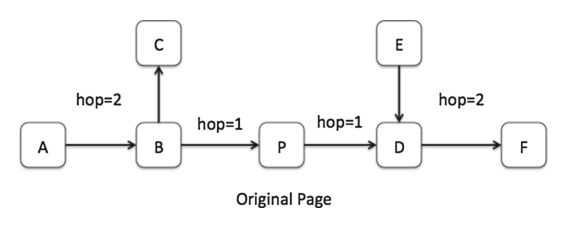
\includegraphics[scale=0.95]{Figures/GenreSim_Draw.eps}
		\caption{GenreSim page selection diagram, found in  \parencite{zhu2016exploiting}.}
		\label{fiig:GenreSim_Draw}
	\end{center}
\end{figure}

\textit{GenreSim} is a ranking algorithm based on \textit{PageSim} algorithm, extended to fit in the problem of genre-taxonomy. Similarly to all this kind of algorithms, is based on the assumption where the more webpages refereed to a particular page, the more this page is related to them in class of topic and/or genre taxonomy. Respectively to the genre-taxonomy the assumption for the GenreSim algorithm, this relation is expended to the level of \textit{forward} $F(p)$ and \textit{backwards} $B(p)$ related URL links. Moreover, the web-pages URL structure is also scored and the pages are characterized as \textit{Hubs} $H(p)$ and \textit{Authorities} $A(p)$. The null hypothesis of the algorithm is that the web pages of the same genre are inter-connected with their URL links. Consequently, a few pages backwards and forwards to a specific web-page consists a "small" network of the same genre. Using this "genre-network", the textual (and partially the structural) information of neighbouring web-pages can be used to amplify the signals required to classify a random page to the proper genre.

\textit{Hubs are pages} with many outgoing URLs, whereas pages with many URLs pointing to, are called authorities. The number of incoming and outgoing URLs are increasing the respective scores as shown in equation \ref{eq:GenreSim_hub_authortities}. However, web-pages with high score but with \textit{few backward URL links} its high likely to be "spam" pages in the context of genre relation. In order to regulate this the $\omega(p)$ factor is intruded of equation \ref{eq:GenreSim_omega}, where is reducing the score for the web pages with few backward links. In addition, it is also normalizing the "few links" issue. That is, the number of the backward links is correlated to the number of links the page itself is containing. 

\begin{equation}\label{eq:GenreSim_hub_authortities}
	\begin{array}{l}
		H(p) = \sum_{u \in V|p \to u} \omega(p) A(u) \\  
    	A(p) = \sum_{v \in V|v \to v} \omega(p) H(u) \\
    \end{array}
\end{equation}
\begin{equation}\label{eq:GenreSim_omega}
	\omega(p) = \frac{N}{|\log N - \log N(p) | + 1} 
\end{equation}
Therefore the score for a random page in the $G$ graph of web-pages, is calculated by equation \ref{eq:GenreSim_Score}. In general the \textit{genre-selection recommendation score} is propagated to the graph path $P(u,v)$ as indicated by the $Score(u, v)$ function of equation \ref{eq:GenreSim_Path}. Therefore, the score of a recommended webpage is decreasing gradually as this pages is farther (in hops) from the web-page to be classified. The $d$ factor is set to be $0.5$, i.e. the page score is decreasing by half for every hop farther from the page under evaluation. 

\begin{equation}\label{eq:GenreSim_Score}
	Score(p) = H(p) + A(p)
\end{equation}

\begin{equation}\label{eq:GenreSim_Path}
	Score(u, v) =
      \begin{cases}
      	\sum_{p \in P(u, v)} \frac{d Score(u)}{\prod_{x \in p, x  \neq v} (|F(x)| +|B(x)|)}, & v \neq u \\
        Score(u), & v = u \\ 
       \end{cases}
\end{equation}
Finally, the similarity of the candidate neighbour pages to the one under evaluation is calculated form equation \ref{eq:GenreSim_Selection_Score}. That is, the ration of the min and the max paths-score sums of all the possible paths, backwards and forwards, to the page under evaluation.

\begin{equation}\label{eq:GenreSim_Selection_Score}
	Sim(u, v) = \frac{\sum_{i=1}^{n} min(Score(v_{i}, u), Score(v_{i}, v))}{\sum_{i=1}^{n} man(Score(v_{i}, u), Score(v_{i}, v))}
\end{equation}
GenreSim is combined with an ML algorithm called MCC (Multiple Classifier Combination). Particularly GenreSim utility is to select a set of web-pages where their content (textual and structural) will be used in combination to the "on-page" content, as an input to the MCC algorithm for classification.

The MCC algorithm is a set of SVM classifiers where each is trained to a particular set of features from the webpage and its neighbours, well selected from the GenreSim, webpages. Then a Decision Template, shown in equation \ref{chap:relevant_work:eq:GenreSim_DP}, is build and used for the classification of a random web-page. Then the Min, Max or Mid values for the classification decision from the matrix are selected for making the final decision for the Genre class of the web-page.

\begin{equation}\label{chap:relevant_work:eq:GenreSim_DP}
	DP(p) = \left(
    	\begin{array}{ccc}
        	d_{11} (p) & \cdots & d_{1|G|} (p) \\
            d_{21} (p) & \cdots  & d_{2|G|} (p) \\
            & \vdots & \\
            d_{N1} (p) & \cdots  & d_{N|G|} (p) \\
         \end{array}
\right)
\end{equation}
\noindent
where $|G|$ is the number of genres in a genre taxonomy and the calcification methods is under a closed set setup with $N$ indented (one for each feature set) \textit{SVM multi-class classifier}. 

Hyperlinks can be exploited by extracting information from the URL string itself and not from the hyper-graph. Particularly, URL can analyzed farther in its components, i.e. \textit{the web-site's domain name, the URI which is the path after the domain and the anchor text}. Special characters such as $\{_ , . , ?, \$ , \%\}$, top-level domains $\{.gr , .uk , .com, etc\}$, and file suffixes such as ".html", ".pdf" are usually discarded and then character n-grams are extracted from the URL counterparts. Finally several weighing schemes were used such as binary, TF or the one described in equation \ref{eq:jebary_url_weigh_cngrams_1} and \ref{eq:jebary_url_weigh_cngrams_2}. WGI experiments using only the hyperlink information combined (or not) with other web-page information seems to be a promising researching path especially for performance oriented WGI applications such as \textit{Genre-Based Focused-Crawling} \parencite{jebari2014pure_URL,jebari2015combination} (MSc reference on focused-genre-crawling)

\begin{equation}\label{eq:jebary_url_weigh_cngrams_1}
	W_{s}(C_{i}, U_{j}) = \sum_{s} w(s) TF(C_{i}, U_{j})
\end{equation}
\noindent
where $TF(C_{i}, U_{j}) $ is the n-gram $C_{i}$ frequency in the $s$ segment of the URL $U_{j}$ and $w(s)$ is weight empirically assigned to the segment depending on the type of the segments as shown in eq. \ref{eq:jebary_url_weigh_cngrams_1}. The weights $\{\alpha,\beta,\gamma\}$ should be defined empirically usually upon the corpus. 
\begin{equation}\label{eq:jebary_url_weigh_cngrams_2}
	w(s) = \left\{
    	\begin{array}{lll}
        	\alpha & if & s = Domain\ Name \\
            \beta & if & s = URL\ path (non\ domain\ part) \\
            \gamma & if & s = Document\ name (e.g. .html, .pdf, etc) \\
         \end{array}
  \right.
\end{equation}
 Another useful source of information is the URL of web documents are in \parencite{abramson2012_URL,jebari2014pure_URL,priyatam2013don_URL}.


\section{The Web Genre units: Section, Page, Site and "Stage"}

AGI/WGI research mostly has studied the genre-taxonomy assuming than a page (or web-page) is mono-thematic, this it has only one genre and only one topic, That is the web pages has been assumed to be the \textit{Genre Unit}. Although, it has been noted in lots of studies that this is not the case. Additionally, the hyperlink and the connection of the web-pages is an other aspect is closely related the genre-units. 

In the  traditional containers such as Books, Document, Posters, Slides, etc; the container itself is the linking of the pages considering the genre. The hyperlinks is replacing the traditional container propriety, respectively the genre taxonomy, and also it extends it. That is, web-pages of them genre are not necessarily belonging to the same web-site, however, they can be linked. Moreover, pages of the same web-site might not be from the same genre. 

In this section the Web Genre units is discussed closely related to the linking of the genre-units and also introducing the notion of \textit{Tracking, Zoning and Sounding} of this units. 

In \parencite{mehler2011integrating} is an study for extracting the \textit{web-page thematic} information by exploiting the semantic linking of the genre-units. In an effort to explore the possibility of creating a \textit{Universal Structure Thematic Structure}, where genre-taxonomies (and topic) would be able to retrieved. Their strategy is exporting the \textit{Linked URL Graph} properties by using the Tracking, Zoning and Sounding graph traversal strategies. In order to extract rich information and finally creating a universal \textit{Genre Retrieval Graph Structure}.

The null hypothesis of the Genre Retrieval Graph is the two level of information can be extracted by the web-pages linking and then mapping this liking to the \textit{Stages} of the page. \textit{Staging} is the process where Sections of the page are extracted which are functioning as taxonomy units. This units are assumed to be mono-thematic. Thus stages are the sections which are sub-genre restricted. Stages for example might be, paragraphs, sentences, bibliography sections, titles, photo gallery, etc. Overall they are defined as the parts of the web-pages with specific sub-genre, for example Bibliography is a sub-genre of \textit{the Academic (and the Publication)} genres.

The web-page linking mapping to the Stages assumes that the linking implies similarity in the taxonomy level, in our case the genre-taxonomy. Then several issues occurring where with Tracking, Zoning and Sounding of the linked graph are tried to be resolved.

\textit{Sounding graph traversal} strategies are used for finding how deep in a \textit{Tree Structured Staged Graph (TSSG)}  the a sub-genre propagates. On the other hand Tracking is the hopes an algorithm should traverse until it reaches the root of the tree.

\textit{Zoning it the process} where the total number of paths are located where only one sub-genre is propagated on the tree. As an example given a web page of a \textit{Market Place} genre, where \textit{products Specification} together with \textit{product Reviews} coexist; sounding is the process where the paths of \textit{the linked Specification} will be separated by the paths of \textit{the linked Reviews}. Note that the assumption of the concept of TSSG is the taxonomy goes beyond the location restriction of a web-site and the sections/stages of the same genre are linked in cross-site manner.

Finally, the process is reduced to the proper staging and and feature/structure encoding on the web-page level, before the TSSG formation. The process is separated in five (5) main sequencs of processing:

\begin{enumerate}
\item \textit{Segmenter process:} where a set of heuristics are applied in order to exploit the HTML markup tags and then forming sections of the webpage that make sense. To do so an algorithm is used where the DOM tree is analysed in its counterparts, together with the respective CSS. Then using an empirical threshold of the size of the text is included in the DOM objects, these objects are re-assembled for reaching the minimum context size.
\item \textit{Tagger process:} where the segments are analyzed for extracting linguistic and superficial features such as; 1) tf-idf term vectors of lexical features, structural features (paragraph size, sentence size ,etc) and HTML markup tag features such as counting the header tags (eg <h1></h1>) etc.
\item \textit{Stage Classification process:} Where several SVM models are trained one for every different Stage. As an example, one for Bibliography sections, one for Schedules, one for Product Review etc.
\item \textit{Disambiguation process:} a Markov-model is applied on each of  HTML Section where the its Stage is calculated based on the \textit{probabilistic grammar} based on the trained SVMs in the step 3.
\item \textit{Web-page Classification process:} where the whole information extracted by the previews steps are given as input to an other page level SVM model, which returns the final decision for the page. 
\end{enumerate}

It has been shown that following the above steps it is possible to reach up to $0.745$ score for $F_{1}$ and $0.694$  \textit{for predicting the sub-genre of the Academic web-sites super-genre }.

\textit{Disambiguation process} is using two types of features the Bag-of-Features (such as BOW, POS, Superficial text features etc) and the \textit{Bag-of-Structures}. Particularly the former is referring to the features extracted directly by the HTML raw text of the segments. The Bag-of-Structures (which is the probabilistic-grammar mentioned above) is a model derived by a the process of an \textit{accumulated transition probability}. To be more specific assuming that the proximity of the segment/stages is relevant; a probabilistic model is calculated for the genres a particular segment is under.

Multi-class classification, hierarchical classification, and multi-page classification is some of the aspects considered in the WGI. Naturally, a web-page, a section on the page, a paragraph on the page, a collection of pages linked together by their URLs. A web-site is, also, a genre-unit. That is, in an experimental set-up one has to consider which genre-unit will be assumed. However, it is foregrounded that in almost any unit there is always a change to be multi-genre \parencite{lee2017text} (also Ashegi, Santini, and other old citations)., for example in \parencite{madjarov2015web} has been found that on average $1.34$ genres are present per web-page.

\section{Focused Crawlers for Genres}\label{chap:relevant_work:sec:focused_crawlers}

Focused crawling, unlike general web-crawling, is the process of downloading only relevant web-pages of \textit{particular topic, genre or query}. As a result valuable time is saved and resources, such as processing power, bandwidth and storage space. Focused crawling engines, i.e. Focused crawlers, are following several strategies and criteria in order to download only the desired pages. The difficulty on the downloading decision is to be made in advance, i.e. before the pages be downloaded \parencite{priyatam2013don_URL} . 
 
Particularly, a genre-focused crawler is possible to be implemented using only the URL's BOW for predicting whether or not a web page will return by this URL will be relevant to genre. To do so a machine learning algorithm should me trained using a well curated training set. Experimental results shown a promising approach with all the affronted benefits for crawling.

There are simple heuristics that could be used in production such as well composed list of words in the URLs strings. Particularly some strategies has been tested where: 1) a list from experts derived, 2) a list of experts augmented using WordNet, 3) list of keywords derived from an "authority" site where the genre-taxonomy is already used for categorizing its content, such as Wikipedia. These heuristic are able to capture some of the required information however is far from a satisfying performance and is a tedious, non-automated and hard to be updated procedure.

An other approach is the machine learning method such as \textit{Nearest Neighbours (NN)} method but in an \textit{Incremental/Adaptive form}. Such as in the case of \parencite{jebari2015combination} this algorithm is adapting the new discovered web-pages when they are above a specific threshold irrespective the similarity score. In could also used an verification algorithm where it could use an other trained model on the webpages contexts. In this manner, after a web paged would have been downloaded the second algorithm could return a verification score in order to be decided whether to adapt the URL or not the the NN model. 

 The main evaluation criterion for the focused crawlers is the \textit{Precision}, although, \textit{Recall} and \textit{Harvest Ratio} are also important \parencite{priyatam2013don_URL}. The task objective is more important the crawled pages to be relevant to the requested genre than potentially missing a few, i.e. high precision and low recall. As we will see later WGI in an open-set framework is focusing mainly on precision performance, which it seems more suitable for the application. 
 
An aspect to be noted is the seeding. Seeding is the initialization procedure where the several URLs are given as starting point for the crawler. First of all usually a manually curated seeding returns faster, and more relevant pages. Secondly main issue for the genre-focused crawling is the \textit{diversity}. That is, \textit{the seed pages should be diverse in respect of the topic} but similar to the genre requested. Several strategies can be used, where the URL string, the webpage content, and the user/authority posting/publishing, are analyzed with machine learning and/or heuristic method for measuring the diversity. Ultimately, exploiting the similarities in context of the above units (URL, Text, Html, Author) a graph is constricted of the \textit{perspective seed pages}. Then an out-of-the box algorithm can be used for finding the pages are connected with a distance greater than three (3) nodes.
 
Measuring the diversity is also an important issue. In the semantic point of view diversity means that a web-page content would be really distant in WordNet distance metric. However, this is not the case, because some specific words, POS n-grams, and other features which are genre-related are also topic-related. Thus \textit{Semantic Distance metric } is not the best choice. On the other hand \textit{Average Similarity between Document-pairs} shown to be more efficient \parencite{priyatam2013don_URL}. 
 
%\textbf{Using the Web as a Corpus - The Genre Approach}
    

\section{Genres Utility}\label{chap:relevant_work:sec:intro}

Genre taxonomy of the texts has a research interest for linguistics and computational linguistics studies, as part of the taxonomy behaviour and evolution. However, is not strictly a tool for studying the languages only academically or as an aiding tool for better NLP and IR results in other domains. It also has its one practical utility directly for the end user. Some examples will follow.

To begin with,  journalism historians have a great interest in the advances of the ML and NLP in order to automatically cluster their resources for better studying the News publication in a systematic historical manner. An closely related study in native and foreign languages teaching is an essential tool for locating documents to be used in the teaching process for developing the competence of written ans spoken language on specific genre. As an example, when the student should learn the difference of academic and casual writing.

An other study for the utility of the genre taxonomy and the \textit{Search Engines Results (SER} is one conducted at Pittsburgh, USA, University.  The experiment measured the correlation of the website's/web-page's genre and the user's preference for completing the task of finding health care information for \textit{Multiple Sclerosis} and \textit{Weight Loss}. The results clearly show that the user's task would be significantly easier if the web resource were organized based on their genre and no only on their topic relation ranking \parencite{chi2018sources}.

Text based genre identification is also a utility for video (e.g. movies, TV series, etc) classification in video/cinematographic genres using the text available such as the subtitles. In this study a variety of ML algorithms has been tested such as SVM, Naive Bayes, Random Forest, Decision Trees and several types of features. Their \textit{content-free} features are equivalent to the superficial features described in section \ref{chap:relevan_work:sec:features}. Moreover, \textit{content-specific} features also used which they are specific words relevant to content\parencite{lee2017text}.

In \textit{Author Profiling} cross-genre evaluation has been employed. That is, texts from a variate of different genres such as \textit{Social Media, Blogs, Twitter and Hotel reviews} used for this task's  \parencite{rangel2016overview}. 

\textit{Office/local documents} multi-faceted search application documents in an office environment (with shared files) was using a genre-taxonomy for aiding the users locating their files. Particularly, their application had great acceptance rate form the users who tested it.  User reported that they were able to locate old slides abandoned more than a decayed related to their current work when using the genre-taxonomy based retrieval. An ensemble based algorithm within an open-set framework was trained, for this task, in a relatively small data-set of 5,098 pages. Then it was tested in a production environment with 30,000 office documents of a 10-year time span. The corpus was including pdf files, images (jpg, png, etc), slides (Powerpoint, Keynote) and HTML booklets \parencite{chen2012genre}.

\section{Web Genre Corpora: An unfinished work in progress}\label{chap:relevant_work:sec:intro}

Santini and Serge in \parencite{santini2009web} for more than a decade have pointed out the problem of the Genre Corpora in the context of the difficulty to be consisted and maintained due to the reasons explained in this chapter up to here. 

The constitution process for the rules required to be followed for composing a text corpus is still a research problem in \textit{linguistics studies}, while the utility of the genre-taxonomy is vividly pointed out. A collection of texts cannot be assumed to be a corpus by default due to several issues should be considered starting with the taxonomy definition where mostly is an overlapping problem, then the texts should have several properties linguistically and statistically defined. The homogeneity in temporal manner, whether are from multiple languages and the way have been collected; \textit{speech, spoken or written corpus}. Particularly speech corpus implies voice recording while spoken means to be transcribed from speech samples. Particularly for the genre-taxonomy the homogeneity related to the time the samples has been collected is very critical since the genres are changing over time until a new genre occurs replacing or dividing from an older \parencite{dash2018history}. Blogs, for example, was the evolution of "personal/memory diaries" when they became public on the web and named "web-logs" then in a second time evolution renamed to "blogs" where their content also changed now is mostly like an \textit{informal journalism} rather than a diary.

The NLP community has overcome the problem of a non-well established corpus of the WGI. There are at least tree publication on the effort on \textit{corpus building methodologies} with vividly different approaches, yet the problem is remaining open due to several issues described in detail in section \ref{chap:relevant_work:sec:linguistics_definition} and in \parencite{melissourgou2017genre,asheghi2014semi} (Ashegi,2018_Book_HistoryFeaturesAndTypologyOfLa_WEB_TEXT_CORPUS.pdf). 

All the approaches are focusing on the genre's main principals, i.e. the function, form and communicative purpose. While in \parencite{asheghi2014semi} the focus was on the semi-automated evaluation procedure in the categorization of the texts, in \parencite{melissourgou2017genre} the process is focusing on the systematic manual process. This process is based on a well established theory of  the Systemic Functional Linguistic (STL) framework where as a shortcut in the process can help on building and evaluating a genre taxonomy corpus. 

There is no drought for the significant contribution of the above studies where all three can be used as the solid framework for building \textit{web-genre-taxonomy corpora} and web-text corpora in general. The utility of the each work can be used as multi-layer filtering process:  1) starting with the automated crawling of the web using focused crawling as explained above \ref{}, 2) Using non-experts crowd-sourcing semi-automated procedures form first level filtering, 3) using the methodology of manual STL based evaluation for fast qualitative analysis and categorization of the post-crowdsourcing-filtered corpus. 

Starting form the final step, in \parencite{melissourgou2017genre} firstly is resolved the ambiguity on the notions related to genre. As they explained the terms "genre", "register", and "text type" are used interchangeably, complimentary and even contradictory, in addition to the debate related to the terms usage. Particularly \textit{text's register, communicative purpose, form} are all components of the \textit{text's genre}, while \textit{text type} is mainly defined by the \textit{text's form}. Alternatively, register is used to describe very general concepts of writing styles such as \textit{formal/informal} while genre mostly includes also the purpose such as \textit{news/blog}, where news' style is mostly formal and blog's informal. Moreover, text's form is also one of the three components of the \textit{register} where it is called "mode" in the context of the register's counterpart. One could attempt to describe the connection of these terms in a mathematical equations such as in equation \ref{eq:genre_notion_in_math}.  

\begin{equation}\label{eq:genre_notion_in_math}
	G  \subseteq P \uplus F \uplus T \uplus M
\end{equation}
\noindent
where $G$ is the genre, $P$ is the communicative purpose and $F, T, M$ are the "register's" components. $F$ is the \textit{field} which answers to the question of \textit{Why?} the text was composed. $T$ is the \textit{tenor} which answers the question of \textit{Who?} or/and to \textit{Whom?} the text was written. $M$ is the \textit{mode} which is the text's form. Note, that G is not exactly equal to their sum of these components of the text, because, some topic counterparts are also genre indicators, although topic is orthogonal to the genre. However, there are several cases where topic indicator are also useful as genre indicators and discussed in section \ref{chap:relevant_work:sec:heuristics}. In addition, we humans recognize the genre by using topic counters parts which it been shown in some cognitive experiments on genre identification in \parencite{clark2014you, lieungnapar2017genre} (briefly explained in section \ref{chap:relevant_work:sec:linguistics_definition}).

Finally, an interesting path towards to the process automating the building of genre-taxonomy corpora is the one found in \parencite{lieungnapar2017genre}. They are using a K-means clustering method as an automated procedure for capturing the possible correlation of \textit{logistic features} and the \textit{Popular Science Sub-Genres}. In their methodology they are using a set of manually extracted linguistic features as presented in table \ref{chap:relevant_work:tbl:pop_science_features} and then they are correlating the z-scores of these features to the possible 4 clusters found to be in the Popular Science \textit{web documents}. Following the same strategy they have managed to show the correlation of the sub-genres to the science disciplines and document sources. Finally they have managed to correlate manually identified genre's function to the linguistic features. Showing that it is possible by using a short of \textit{funnel like Filter} is possible to gradually extract higher and more abstract levels of information starting with the linguistic features, continuing with function features (or text-registers) (e.g. Impersonal, Narrative, Persuasive, Informative, Elaborated, Impersonal) and finally classifying the genres. Finally, they have shown that their final evaluation to their semi-automated process was as good as the experts agreement on the same task after they have manged to form a "golden standard" manually. 


\section{Discussion and Future Work Suggestions}\label{chap:relevant_work:sec:intro}

\begin{itemize}
\item Semi-automated corpus bundling.
\item Metrics for evaluating the corpora qualities such as diversity, topic to genre orthogonal properties, etc.
\item ML with built-in feature selection properties.
\item Open-set Semi-supervised clustering.
\item Web-documents linked Graph visualization with URL and Genre connection.
\item Random Term Feature Selection can it be "beaten" by the Neural Language Models, i.e. is there a case of NLM where they can behave significantly better than random selection? NLM seem worst or equal (but not better) than random features because of the limited available corpora for WGI or is a task oriented issue?
\end{itemize}


























%!TeX spellcheck = en-US

%\chapter{Open-set and Closed-Set Classification for WGI}
\chapter{Open-set WGI algorithms}

\label{chap:openset}

%----------------------------------------------------------------------------------------

% Define some commands to keep the formatting separated from the content
\newcommand{\keyword}[1]{\textbf{#1}}
\newcommand{\tabhead}[1]{\textbf{#1}}
\newcommand{\code}[1]{\texttt{#1}}
\newcommand{\file}[1]{\texttt{\bfseries#1}}
\newcommand{\option}[1]{\texttt{\itshape#1}}

%----------------------------------------------------------------------------------------

\section{Introduction}\label{chap:openset:sec:intro}


In this chapter three open-set algorithms are described in detailed where they have been developed for the WGI task. These algorithms is an algorithmic extension of the most popular closed-set algorithms and basic approaches one can follow. Although, their base algorithms are trivial their open-set extension are covering some sophisticated issues of the \tetxit{Automated Genre Identification} and specifically the WGI. 

Particularly, the \tetxit{One Class SVM Ensemble (OCSVME)} has been developed which is an extension of the One Class SVM (OCSVM) where the later is also an extension of the $\nu$-SVM. Note that SVM is design for closed-set classification scenario and also the $\nu$-SVM. The OCSVM is a form of binary classifier with the special case where only positive samples are available for the training phase. Also, only the center of the vector space and few of the positive examples (called outliers), are considered as negative examples. The OCSVME is an open-set and multi-class classification form of the SVM which fits the WGI task. 

The \textit{Random Feature Subpacing Ensemble} is an other algorithm developed for this thesis, for fitting the open-set scenario of the WGI task. This is a distance based algorithm where a random set of features is selected for comparing the distance of the class and an arbitrary document. Several distance measures can be used such as the \textit{Cosine, Min-Max, Euclidean, Mahalanobis, etc}. The distance based algorithms seem to work very efficiently for WGI as in several text mining problems with high dimensional space.

The \textit{Nearest Neighbors Distance Ratio (NNDR)} is the final algorithm developed in this thesis specially for WGI task. It is based on the same NNDR developed for \parencite{} which also is special case of the \tetxit{Nearest Neighbor (NN)} for fitting the open set scenario. 

As explained in chapter \ref{chap:relevant_work} there are several issues relate to the WGI. Every of the above algorithms has been developed for tackling the major ones in respect of the Machine Learning bound issues perspective. 

Considering the experimental set-up in the WGI there are two issues. Firstly, the Genre domain is practically infinite due to the constantly emerging new genre and their temporal manner where they are reformed through time. Secondly, due to the great scale of the Web it is impossible to collect a characteristic statistically correct negative set of examples. Although, there is a plethora of positive examples for a genre. The OCSVME has been developed in this issues in mind. Since, it can work with only positive examples and also can work in a open-set framework of experiments.

The second issue is the great dimensionality where is a general text mining issues. However, for WGI the constrains of the very small scaled corpora available for the very high scale problem considering the Web. Moreover, in section \ref{chap:relevant_work:sec:features} it is discussed that the main research focus was around the problem of the proper feature selection for the WGI. Having this in mind the RFSE is a competent algorithm for selecting the proper features implicitly based on the majority statistics. It can also work in the open-set framework.

The open-set classification itself is opening an other difficulty which is called the \textit{Open Space Risk (OSR)}. That is, the risk of placing the decision boundaries too far or close due to the presences of Outages the luck of \tetxit{Negative samples} and the \textit{(structured or unstructured) Noise}. The NNDR has originally developed having the regularization of the OSR in mind and in this thesis it has been specially developed of the WGI task.

Finally, all three algorithms have been developed with Noise handling and Outages tolerance in mind. Specifically, all three algorithm can be tuned to regulate their Noise filtering ability with an explicit or implicit threshold. The Noise as explained earlier can be structured or unstructured, i.e. when the noise samples are balanced or not in respect of the genre tags. Note that the noise-filtering regularization threshold is automatically defined for NNDR while training using the OSR as a measure.


In the rest of this chapter a section is dedicated for one of every algorithm starting with the OCSVM as prerequisite for explaining the open-set flowing algorithms.


\section{One-class Closed-set Classification Methods}\label{chap:openset:sec:One_Class_Classification}


The main difference of the One Class Classification problem (OCC) with respect to the conventional multi-class or binary classification problem is that in OCC there are only available positive examples of a class and none or very few negative examples. There are several approaches towards the solution of this problem. A compact survey on OCC is provided by Khan et al.\parencite{khan2010survey}. 

To begin with there are several references to the well known \parencite{scholkopf1999estimating} which actually presents an alternative solution to the problem of \textit{the overlapping samples distributions}, known as $\nu$-SVM \parencite{bishop2006}. The nature of $\nu$-SVM is allowing us to use it effortless in binary classification problems as long as to OCC problems. The parameter $\nu$ is both controlling the fraction of SVs and the \textit{margin errors}, i.e. point out the positive sample considered as outliers. 

In the case of OCSVM the optimization process begins with considering, as the only negative example, \textit{the origin} of the vector space defined from the \textit{data space}. More details for OCSVM are given into the section \ref{chap:openset:sec:OCSVM_description}.

Outlier-SVM is an OCSVM the algorithm of \parencite{manevitz2002one,khan2010survey}. In their algorithm the \textit{Hamming distance} has been used. Their model was competitive but not top performer when comparing their model to other OCSVM algorithms such as One Class Neural Networks, One Class Naive Bayes Classifier, One Class Nearest Neighbor, and Rocchio Prototype. In addition their algorithm is sensitive to the term weigting schema, i.e. \textit{Binary, TF, TF-IDF, etc.}, and vector dimensionality. 

The \textit{Rocchio's algorithm} is the simplest one class classification algorithm where it has been used for IR problems because of its simplicity and consistency \parencite{joachims1997probabilistic}. The learning process is just the summation of all the sample vector of a class, i.e the \textit{prototype vector}. An arbitrary vector is classified as positive or negative using the angular distance from the prototype vector.

Datta (cited in \parencite{manevitz2002one}) proposed Naive Bayes Classifier modification for OCC problems and use only positive samples in the learning process. A \textit{probability density function} of a class $E$ is induced as prediction model. Classifying the a document $d$ involves calculating the probability of the document $p(d|E)$ which is equal to the product of its features $w_{n}$ probabilities $p(w|E)$, where $n$ is the number of document's feature vector. To decide weather the document is classified as positive its required a threshold. 

There are, also, some OCC methods exploiting the availability of \textit{unlabeled data} as the following cases. 

\parencite{yu2005single} proposed two OCC algorithms that use positive and \textit{unlabeled data} for building a classification model that describes the \textit{single class boundary}. The \textit{Mapping Convergence }(MC) algorithm is incrementally labeling negative data from an \textit{unlabeled data set} using the margin maximization property of SVM. The \textit{Support Vector Mapping Convergence} (SVMC) optimizes the MC algorithm for fast training. Both algorithms had been compared into a real world text classification, letter recognition, and diagnosis of breast cancer with higher performance that other similar algorithms. These similar algorithms are \tetxit{Spy Expectation Maximization (S-EM), SVM-NN (i.e. C-SVM using unlabeled data point as negative ones) and Naive Bayes Classifier with noise sampels} \parencite{liu2002partially, li2003learning}.

To conclude, the one class classification is facilitating the problem of only positive available samples either for the one-vs-rest case \parencite{khan2010survey,manevitz2002one,yu2005single,scholkopf1999estimating,li2003learning}. In the next chapter (\ref[chap:openset:sec:Openset_Class_Classification) the open-set classification problem is discussed and the three algorithm developed for this thesis are presented in detail.



\section{Open-set Classification}\label{chap:openset:sec:Openset_Class_Classification}

In this chapter three open-set algorithms developed for this thesis are discussed in detail where their evaluation experiments will be presented in chapter \ref{chap:noise}. 

The open-set classification in this thesis primarily employed to handle the Noise. The

...


\begin{definition}{\textit{Open-set Identification}}
describes a scenario where samples of unseen, in training phase, classes appear in testing phase. Then the classifiers classify accurately the the \textit{known classes} and also effectively deal with the unknown ones. Therefore, the classifiers need to have a \textit{rejection option} when an arbitrary sample is from an unknown class \parencite{geng2018recent}.
\end{definition}

Although, the rejection option is emphasized in the definition of the open-set identification, the algorithms with rejection option are not open-set by default. Particularly there are several scenarios such as in \parencite{onan2018ensemble} where this option is used for rejecting the outages for improving the precision score. However, the framework remains as closed-set.

Open-set classification framework is closely related to the \textit{Novelty Detection} and the \textit{One-class Classification} where it is assumed that only positive examples are available for the surprised model induction methods. These methods then have been adapted to this problem and there are several examples such as One-Class SVM, One-Class Neural Networks....


...


The {Open-Space Risk} is a definition form the domain of Open-Set classification research to describe the weakness of the current closed-set ML algorithms usually are used out-of-the-box to regulate low Recall performance of the models due to the luck of negative samples. In order to measure the performance of such algorithms the \textit{Openness} test have very recently introduced. 

A more formal definition of the Open-set classification is the one where the open space risk is considered.

%\theoremstyle{definition}
\begin{definition}{\textit{Open-set Multi-class Classification}}

Let $C$ be the training data, and let $R_{O}$ open space risk and $R_{ε}$ the empirical risk. Then the objective of open-set classification is to find a function $f \in L$ which is minimizing the following \textit{Open-Set Risk}. 

Mathematically described as $arg_{min} \{R_{O(f )} + \lambda R_{ε (f (V ))}\}$, where $f (x) > 0$ implies correct recognition and $\lambda$ is a regularization constant.

Thus \textit{open-set risk} balances the \textit{empirical risk} and the \textit{open space risk} over the space of allowable recognition functions \parencite{geng2018recent}.

\end{definition}

In practice the \textit{empirical risk} is the weighted loss function of the open-set multi-class classification model. The \textit{open space risk} is in practice the ratio of the open vector space to the full vector space, where the full vector space is the concatenation of the space defined by the known data samples and the unconstrained unknown space.


...



\subsection{One-Class SVM Ensemble}\label{chap:openset:sec:OCSVM_description}

One-class SVM is actually an $\nu$-SVM for the case we want to find the contour which is prescribing the positive samples of the training set given for a single class, while there are \textit{no negative samples}. nu-SVM ($\nu$-SVM) is providing an alternative \textit{trade-off control method of misclassification}, proposed from Scholkopf et al. \parencitep{scholkopf1999estimating}. In $\nu$-SVM we are minimizing eq.\ref{eq:3} with the constraints of eq.\ref{eq:4}, eq.\ref{eq:5}.

Following the logic from the conventional SVM, thoroughly analysed in \parencitep{bishop2006}, the Lagrange multipliers for solving the optimization problem of eq.\ref{eq:3} under eq.\ref{eq:4}, eq.\ref{eq:5} constraints are used. Equation \ref{eq:12} is then derived, i.e. a Lagrangian function to be maximized as subject to the constraints eq.\ref{eq:4}, eq.\ref{eq:5}.

\begin{equation}\label{eq:3}
	arg\min_{w,b}\left\{ \frac{1}{\nu\lambda}\sum_{n=1}^{N}(\xi_{n}-\rho)+\frac{1}{2}\|w\|^{2}\right\}
\end{equation}

\begin{equation}\label{eq:4}
	0\leqslant a_{n}\leqslant1/N,\qquad n=1,...,N
\end{equation}

\begin{equation}\label{eq:5}
	\nu\leqslant\sum_{n=1}^{N}a_{n}, \qquad \sum_{n=1}^{N}a_{n}t_{n}=0
\end{equation}

\begin{equation}\label{eq:12}
	\widetilde{L}(a)=-\frac{1}{2}\sum_{n=1}^{N}\sum_{m=1}^{M}a_{n}a_{m}t_{n}t_{m}k(x_{n,}x_{m})
\end{equation}

\newpage


It should be noted that $\nu$ in $\nu$-SVM has the flowing properties:
\begin{itemize}
	\item $\nu$ is an upper bound on the fraction of \textit{Outliers}.
	\item $\nu$ is a lower bound on the fraction of \textit{Support Vectors}.
	\item $\nu$ values cannot exceed 1 (see eq.\ref{eq:4}).
\end{itemize}

In practice different values of $\nu$ are defining different proportion of the training sample as outliers. For example in \parencitep{scholkopf1999estimating} is showed that in their experiments when using $\nu=0.05$, 1.4\% of the training set has been classified as outliers while using $\nu=0.5$, 47.4\% is classified as outliers and 51.2\% is kept as SVs.

In the prediction phase in order for an OCSVM model to decide whether a document is belonging to the target genre-class (or not) a \textit{decision function} is used. The decision function indicates the distance of the document, positive or negative, to the hyperplane separating the classes. In the case of OCSVM we are usually only interested whether the decision function is positive or negative for deciding if an arbitrary document belonging or not to the target class.

In this work we are using the OCSVM in an ensemble form, first proposed in \parencitep{pritsos2013open}, as analytically described in algorithm \ref{alg:OCSVM-Ensemble}. There we are both interested in the positive and negative decision of each ensemble's classifier, and the decision scores.

\hfill \break

\begin{algorithm}[H]
\caption{The \textit{OCSVM} algorithm.}\label{alg:OCSVM-Ensemble}
\KwData{ $G$ a genre palette and $W_{g}$ a set of known web-pages for each $g \in G$,
		 $w$ an unknown webpage of the $W_{a}$ arbitrary webpages set,
		 $F$ the feature set,
		 $\boldsymbol\nu$ the nu hyper-parameter of OCSVM,
         }
\KwResult{ $r \in \{G,\,\emptyset\}$ }
$score[:, :]$=0, the score 2D matrix where rows are for genre's class tags and columns for each webpage under evaluation
\For{each $g \in G$}{
  $Model(g) = ocsvmTrain(W_{g},F,\boldsymbol\nu)$, train a OCSVM model in vector space $F$ with hyper-paramenter $\boldsymbol\nu$ for genre $g$\;
}
\For{each $g \in G$}{
    \For{each $w \in W_{a}$}{
        $score[g, w] = ocsvmApply(Model(g),F,w)$, the distance of the unknown page $w$ from the hyperplane\;
    }
}
\eIf{$max(score[:, :])< 0$}{
    $r \in \emptyset$, i.e. none of the known genres or "I don't know";
}
{
        $r = argmax_{g \in G}(score[:, :])$, i.e. $w$ belongs to the genre of highest score\;
    }
\end{algorithm}

\hfill \break


In training phase of the ensemble one OCSVM is built for each known genre label. The hyper-parameter $\nu$ has the same value for all OCSVM models. In the prediction phase, the document is assigned to the class with the highest positive distance from the hyperplane (or the contour for OCSVM). If all OCSVMs return a negative distance (i.e. the web-page does not belong to this genre) the document remains unclassified, that is the final answer corresponds to "I Don't Know". The OCSVM ensemble was implemented in Python using the \textit{scikit-learn}\footnote{http://scikit-learn.org} package.

\subsection{Random Feature Subpacing Ensemble}\label{sec:RFSE_Description}

The RFSE algorithm is a variation of the method presented by Koppel et al. \parencitep{koppel2011authorship} for the task of \textit{author identification}. In the original approach, there is only one training example for each author and a number of simple classifiers is learned based on random feature subspacing. Each classifier uses the cosine distance to estimate the most likely author. The key idea is that it is more likely for the true author to be selected by the majority of the classifiers since the used subset of features will still be able to reveal that high similarity. That is, the style of the author is captured by many different features so a subset of them will also contain enough stylistic information. Since WGI is also a style-based text categorization task, this idea should also work for it.

\hfill \break

\begin{algorithm}[H]
\caption{The \textit{RFSE} algorithm.}\label{alg:RFS-Ensemble}
\KwData{ $G$ a genre palette and $W_{g}$ a set of known web-pages for each $g \in G$,
		 $w$ an arbitrary web-page of the $W_{a}$ arbitrary webpages set,
		 $F$ the feature set,
		 $fs$ a fraction of feature set size,
		 $I$ a number of iterations,
		 $\boldsymbol\sigma$ the decision threshold }
\KwResult{ $r \in \{G,\,\emptyset\}$ }
\For{each $g \in G$}{
  $centroid[g] = average(W_{g},F)$, average all known web-pages $W_{g}$ of genre $g$ to build a centroid vector\;
  $score[g]=0$\;
}
\Repeat{$I$ times}{
    $f = subset(F,fs)$, Randomly choose $fs$ features from the full feature set $F$\;
    \For{each $g$ in $G$}{
        \For{each $w$ in $W_{a}$}{
    	   $sim[g, w] = similarity(w, centroid(g), f)$, estimate similarity of unknown page $w$ with $centroid(g)$ in vector space $f$\;
        }
    }
   	$maxg = argmax_{g \in G}(sim[:, :])$, find the top match genre\;
   	$score(maxg) = score(maxg) + 1$, increase the score of top match genre\;
}

\eIf{$max(score(g))/I > \boldsymbol\sigma$}{
   $r = argmax_{g \in G}(score(g))$, assign the unknown page to genre with maximum top matches\;
}
{
      $r = \emptyset$, none of the known genres or "I don't know"\;
}
\end{algorithm}

\hfill \break

In our study we adopt the RFSE method as introduced in \parencitep{pritsos2013open} shown in \textit{Algorithm \ref{alg:RFS-Ensemble}}. There are multiple training examples (documents) for each available genre. To maintain simplicity of classifiers, we have used a \textit{centroid vector} for each genre. In the training phase, a centroid vector is formed, for every class, by averaging all the Term-Frequency (TF) vectors of the training examples of web pages for each genre.

The class centroids are all formed for a given feature type. Then, an evaluation document is compared against every centroid and this process is repeated $I$ times. Every time a different feature sub-set is used. Then, the scores are ranked from highest to lowest and we measure the number of times the document is top-matched with every class. The document is assigned to the genre with maximum number of matches given that this score exceed a predefined $\sigma$ threshold. In the opposite case, the document remains unclassified, the RFSE responds "I Don't Know".


With respect to the similarity function, we examine cosine similarity (similar to \parencitep{pritsos2013open}) and MinMax similarity (inspired by \parencitep{koppel2014determining}). Moreover, in this paper we introduce a measure that combines these two similarity functions and selects the one that is most confident in each iteration. More specifically, since cosine and MinMax may have different mean and standard deviation for the set of all evaluation documents and all iterations per document, we first normalize their value. Then, for each evaluation document and each iteration we select the one with maximum normalized value. We call this similarity measure \textit{Combo}.

\section{Nearest Neighbors Distance Ratio}\label{sec:NNRD_Description}

The Nearest Neighbors Distance Ratio (NNRD) algorithm is our variant implementation of the proposed open-set algorithm of Mendes et al. \parencite{mendesjunior2016}. In the original approach euclidean distance has been used because of the variation of data set on which the algorithm has been evaluated. In our approach we are using cosine distance, because in text classification is being confirmed to be the proper choice in hundreds of publications. Moreover, the cosine distance is comparable to the results of the \textit{Random Feature Sub-spacing Ensemble} algorithm found in \parencite{pritsos2018open} where cosine similarity is used for the WGI evaluation.

The NNRD algorithm is an extension of the simple \textit{Nearest Neighbors} NN algorithm where additionally to the sets of training vectors (one set for each class) a threshold is selected by maximizing the \textit{Normalized Accuracy} (NA) as shown in equation\ref{eq:NA}) on the \textit{Known} and the \textit{Marked as Unknown samples}.

\begin{equation} \label{eq:NA}
    NA = \lambda A_{KS} + (1 - \lambda) A_{MUS}
\end{equation}

\noindent
where $A_{KS}$ is the \textit{Known Samples Accuracy} and $A_{MUS}$ is the \textit{Marked as Unknown Samples Accuracy}. The balance parameters \lambda regulates the mistakes trade-off on the known and marked-unknown samples prediction.

The optimally selected threshold is the the \textit{Distance Ratio Threshold} (DRT) where NA is maximized. Equation \ref{eq:DR} is used for calculating the Distance Ratio (DR) of the two nearest class samples, say $s_{c_{a}}$ and $u_{c_{b}}$, to a random sample $r_{x}$ under the constrain $c_{a} \notequal c_{b}$, where $c_{g}$ is the sample's class.

It is very important to note that the $c_{g}$ is trained in an open-set framework, therefore, the samples pairs selected for comparison might either be from the known of the marked as unknown samples. Thus $g \in {1,2,...,N}$ and $g = \emptyset$ when samples is marked as unknown.

\begin{equation} \label{eq:DR}
    DR = \frac{D(r_{x}, s_{c_{a}})}{D(r_{x}, s_{c_{b}})}
\end{equation}
\noindent
where $D(x,y)$ is the distance between the samples where in this study is the \textit{Cosine Distance}.

Therefore, the fitting function of the NN algorithm, described in pseudo-code \ref{alg:NNDR_fitting}, is the optimization procedure to find the DRT values for classes respective sets of training samples where NA is maximized.

\hfill \break

\begin{algorithm}[H]
\caption{\textit{Nearest Neighbor Distance Ratio} training data fitting function}\label{chap:openset:alg:NNDR_fitting}
\KwData{$G$ the set of genre class tags $\{1,2,...,N\}$,
        $p$ the hyper-parameter regulates the percentage of $G$ tags will be marked as unknown,
        $k$ the hyper-parameter regulates the percentage of known $G$ tags that will be keept for validation only,
        $T$ the \textit{Distance Ratio} thresholds set than will test for finding the one which is minimizing the \textit{Normalized Accuracy},
        $\lambda$ regulates the mistakes trade-off on the known and marked-unknown samples prediction (see eq.\ref{eq:DR}),
        $C[g]$ the matrix of class vector sets one for every genre class tag $g \in G$}
\KwResult{$DRT$ the \textit{Distance Ration Threshold} calculated by the NNRD algorithm's fitting function, $C[g]$}

$K^{G}_i, K^{G}_{validation}_i, U^{G}_{validation}_i, I^{G} = Split(G,p,k)$ splitting the $G$ tags in to known/unknown samples combinations using the $p$ and $k$ hyper-parameters. The amount of split combinations is calculated by the equations \ref{eq:splt_percent} and \ref{eq:splt}.\;

$V^{G} = U^{G}_{validation} \cup K^{G}_{validation}$ the validation set is the union of the $I$ splits of the known-validation and the marked-as-unknown sets, of the whole training set\;

\For{each $i \in I$}{
    $D^{cos}_{VK}[i] = COS_{D}(V^{G}_i, K^{G}_i)$ calculating all the Cosine Distances between the web-page of $K^{G}$ and $V^{G}$ sets for \textit{every $I$ split combination};
}

$Ci^{min}_{A} = argmin(D^{cos}_{VK})$ getting the indices of the closest classes from $V$\;
$Ci^{min}_{B} = argmin(D^{cos}_{VK})$ getting the indices of the \textit{second closest} classes from $V$\;

$R_{V} = D^{cos}_{VK}[Di^{min}_{A}] / D^{cos}_{VK}[Di^{min}_{B}]$ calculating the Distance Rations $R$ for all the vectors in $V$

$NA^{max} \gets 0$ initializing \textit{Maximized Normalized Accuracy} with $0$ value.
$DRT \gets 0$ initializing \textit{Distance Ratio Threshold} with $0$ value.

\For{each $drt \in T$}{

    \For{each $r, i \in \{R_{V}, count(R_{V})\}$}{

        \eIf{$r < drt$}{
            $vi = Ci^{min}_{A}[i]$ keep the respective index\;
            $Y[i] = G[vi]$ setting the genre's class tag as prediction for this random vector of set $V$\;
        }
        {
            $Y[i] = \emptyset$ setting as none of the known genres or "I don't know"\;
        }

    }

    $NA_{V} = NormalizedAccuracy(Y, R_{V})$ calculating the Normalized Accuracy as shown in equation \ref{eq:NA} for tested threshold $drt$\;

    \eIf{$NA_{V} > NA^{max}$}{
        $NA^{max} \gets NA_{V}$ keeping the maximum $NA$ until the outer for-loop finishes\;
        $DRT \gets drt$ keeping the \textit{Distance Ratio Threshold} maximizes the \textit{Normalized Accuracy}\;
    }

}

\end{algorithm}

In the optimization procedure the training samples are split based on their class tags $c_{x}$. Then some class tags are \textit{marked as unknown} and some are left being known. Therefore, all the samples of the marked as unknown are used only in the validation subset while the known class tags samples are farther split into the classes sets (one for each class) and into the known validation set. Then, samples of the validation sets, both then known and then marked as unknown, are used seamlessly for calculating the set of Distance Rations (one for each class). Afterwards, a set of DRT values are tested given a range of values $R \in {t_{1}, t_{2}, t_{n}}$ beforehand where the $t_{x}$ is selected which is maximizing the NA of the validation set.

The splitting procedure the of the training set is regulated by a hyper-parameter $p$ which defines the percentage of the class tags set $g \in {1,2,...,N}$ where they will be marked as unknown. Then the total number of all possible splitting combination are calculated and these split-sets are used for finding the DRT. The combination are found using equations \ref{eq:splt_percent} and \ref{eq:splt}, where eq.\ref{eq:splt} is the \textit{Binomial Coefficient}.

\begin{equation} \label{eq:splt_percent}
    U_{num} = int(N * p)
\end{equation}

\noindent
where $N$ is the size of the class tags set ${1,2,...,N}$ and $p$ is the percentage regulation parameter for keeping the number of tags to be marked as unknown.

\begin{equation} \label{eq:splt}
    S_{num} = \frac{N!}{U_{num}!(N-U_{num})!}
\end{equation}

The NNDR is a open-set classification algorithm, therefore, every random sample will be classified to one of the classes the NNRD has been fitted or to the unknown when its DR is greater then DRT. While training as explained above the DRT values are tested incrementally until the optimal data fitting for the training function.

In prediction phase the DRT is passed to the NNDR prediction function together with the random samples and the training samples as shown in pseudo-code \ref{alg:NNDR_prediction}.

\begin{algorithm}[H]
\caption{\textit{Nearest Neighbor Distance Ratio} prediction function}\label{alg:NNDR_prediction}
\KwData{ $W$ the vector set of the random web-page to be classified,
         $C[g]$ the matrix of class vector sets one for every genre class tag $g \in G$,
		 $DRT$ the \textit{Distance Ration Threshold} calculated by the NNRD algorithms fitting function}
\KwResult{ $Y \in \{G,\,\emptyset\}$,
           $R$ the Distance Ratio scores vector, one score for every input vector of the random set $W$}

\For{each $g \in G$}{
    $D^{cos}_{C_{g}X} = COS_{D}(C[g], X)$ calculating all the Cosine Distances between the random web-page vectors and the class vectors of class $g$\;
}

$Ci^{min}_{A} = argmin(D^{cos}_{C_{g}W})$ getting the indices of the closest classes from $W$\;
$Ci^{min}_{B} = argmin(D^{cos}_{C_{g}W})$ getting the indices of the \textit{second closest} classes from $W$\;

$R_{W} = D^{cos}_{C_{g}W}[Di^{min}_{A}] / D^{cos}_{C_{g}W}[Di^{min}_{B}]$ calculating the Distance Rations $R$ for all the vectors in $W$

\For{each $r, i \in \{R_{W}, count(R_{W})\}$}{

    \eIf{$r < DRT$}{
        $vi = Ci^{min}_{A}[i]$ keep the respective index\;
        $Y[i] = G[vi]$ setting the genre's class tag as prediction for this random vector of set $W$\;
    }
    {
        $Y[i] = \emptyset$ setting as none of the known genres or "I don't know"\;
    }

}

\end{algorithm}

Our implementation of the above NNRD algorithm can be found at \url{https://github.com/dpritsos/OpenNNDR}, where it is implemented in Python/Cython and can significantly accelerated using as much as possible CPUs due to its capability for concurrent calculations in C level speed. Since, NNRD is a rather slow classification method, we have seen in practice that there is up to 100 time acceleration from the capability to exploit a cloud service with 32 vCPUs (Xeon) compare to 4-core/8-threads i7 CPU.

%!TeX spellcheck = en-US

%\chapter{Evaluation Methodology for WGI and Computational Text Categorization}
\chapter{Evaluation framework for open-set WGI}

\label{chap:eval_methods}

%----------------------------------------------------------------------------------------

% Define some commands to keep the formatting separated from the content
\newcommand{\keyword}[1]{\textbf{#1}}
\newcommand{\tabhead}[1]{\textbf{#1}}
\newcommand{\code}[1]{\texttt{#1}}
\newcommand{\file}[1]{\texttt{\bfseries#1}}
\newcommand{\option}[1]{\texttt{\itshape#1}}

%----------------------------------------------------------------------------------------

\section{Introduction}\label{chap:eval_methods:sec:intro}

This chapter is describing the evaluation metrics required for the open-set WGI task. Particularly it is shown with simple examples the effect of the a measurement methods to the evaluation results and the misleading conclusions on can have when the wrong measurement method is adopted. Moreover some evaluation measures are presented specialized for the open-set framework where recently have been discover and adopted for several domains inside and outside the \textit{text mining} domain.

The standard evaluation approach is to use a previously well tested evaluation methodology and measures. However, the closed-set measures is later shown that they are not proper for the open-set framework in their standard form. 

To reason it in few words the problem is that these measures are based on the \textit{Confusion Matrix} which can capture only two condition per variable. However, in the case of open-set framework there is one say "global" condition where all the variables of the table drops. This condition is occurring when the \textit{rejection condition} of the open-set algorithm is triggered. That is when an open-set algorithm responds "I don't know" for an arbitrary sample. 

As explained in chapter \ref{chap:openset} there are some efforts to crate open-set algorithms than could model the \textit{unknown} or \textit{unstructured noise} samples. In this case it could be possible the out-of-the-box closed-set evaluation methods be sufficient,however, in most ML algorithms where a rejection criterion is considered this is nearly impossible as it will be presented later.

\section{Closed-set vs Open-set Measures}\label{chap:eval_methods:sec:measures} 

In this section it is presented how the text mining evaluation measures are affected by the type of the by the type of the task's approach scenario. That is, whether i
t is an open-set of closed-set classification framework.

Starting with the \textit{Confusion matrix} where the basic closed-set evaluation measures are based it is shown the difference in measure of the Precision and Macro-Precision difference (also for Recall) in the open-set framework. Moreover, it is shown how these measures are affected by he openness score which is the score for evaluating the difficulty level of an open-set problem.

Finally, the \textit{Open Space Risk} is presented which is the measure helping an open-set algorithm to regulate the potentially error in the presence of \textit{noise} in the testing or/and \textit{outages} in the training phase.


\subsection{Confusion Matrix and $F$ Score}\label{chap:eval_methods:sec:prf_micro}

In Machine Learning (and Statistical) Classification, a \textit{Confusion Matrix} is a table that depicts the performance of an algorithm. It is a special case of a \textit{Contingency Table}, with two dimensions, actual and predicted classes. Thus, in the a binary case such as in the table \ref{chap:eval_methods:tbl:bin_confusion}, there are for cases occurring. True Positive (TP), True Negative (TN), False Positive (FP), False Negative (FN).

In the case of binary classification the samples under the class distribution A are desired, i.e. positive, and all the other samples outside the distribution are considered negative, classified in say class B. Then TP and TN are the counts of samples predicted correctly under the a class A (positive) or class B (negative). Therefore, the FP and FN are the samples a binary algorithm misleaded and predicted the wrong class. 

\begin{table}[H]
	\center
	\caption{Confusion matric of binary classification}\label{chap:eval_methods:tbl:bin_confusion}
	\begin{tabular}{c c c c c}
		& & \multicolumn{2}{c}{Actual} & \\
		\cline{3-4}
		\multirow{3}{*}{\rotatebox[origin=r]{90}{Predicted}} & & \multicolumn{1}{|c}{A} & \multicolumn{1}{c|}{B} & \\
		\cline{2-4}
		& \multicolumn{1}{|c}{A} & \multicolumn{1}{|c}{\textbf{50}} & \multicolumn{1}{c|}{30} & 80 \\
		& \multicolumn{1}{|c}{B} & \multicolumn{1}{|c}{25} & \multicolumn{1}{c|}{\textbf{35}} & 60 \\
		\cline{2-4}
		&  & 70 & 70 & \textbf{85}\\
	\end{tabular}
\end{table}

In order to measure the performance a binary classification algorithm the \tetxit{Accuracy} is a common measure which is actually the ration of all the correct prediction overall the predictions (which is equivalent to the number of the samples of the whole data set). Formally, it is shown in the equation \ref{chap:eval_methods:eq:accuracy} and for the example of the table \ref{chap:eval_methods:tbl:bin_confusion} its value is $A = 85/140 = 0.607$

\begin{equation}\label{chap:eval_methods:eq:accuracy}
A = \frac {TP + TN} {TP +  TN + FP + FN}
\end{equation}

However, one can get a better insight when it is measured the algorithms ability distinguishing the samples which they are under the distribution it has been trained for. Moreover, to be measured its ability of recognizing the samples of this distribution. The former is called \textit{Precision} and the second it is called \textit{Recall} and their formal expressions are in equation \ref{chap:eval_methods:eq:precision} and \ref{chap:eval_methods:eq:recall} respectively. 

\begin{equation}\label{chap:eval_methods:eq:precision}
	P = \frac {TP} {TP + FP}
\end{equation}

\begin{equation}\label{chap:eval_methods:eq:recall}
	R = \frac {TP} {TP + FN}
\end{equation}

\textit{Precision} is also known as \textit{Positive Predictive Value (PPV)}. \textit{Recall} is also known as \textit{Sensitivity, Hit Rate and True Positive Rate (TPR)}. Again based on table \ref{chap:eval_methods:tbl:bin_confusion} the precision is the ration its first cell value and the sum of its first row (prediction) which is equal to $p = 50 / 80 = 0.625$. Similarly, recall is equal to the ration of first cell value over the first column, i.e. $r = 50 / 70 = 0.714$

So far one-class closed-set classification was considered where the class A was the positive outcome and the Class B the negative. In the multi-class closed-set classification scenario, an algorithm is trained for both A and B class distribution. Thus, the positive and negative samples are now counted from both classes.

In the same table \ref{chap:eval_methods:tbl:bin_confusion} the \textit{precision} and \textit{recall} is now calculated by the ration of the diagonal sums of all positive and all expected respectively. That is $p = 85 / (80 + 60) = 0.607$ and $r = 85 / (70 + 70) = 0.607$. 

If one would like to consider the performance on class A separately to the performance on class B then the respective calculations are for precision and recall. The ration of the A correct predictions over the whole positive prediction of row A and similarly for B. Thus, $p_{A} = 0.625$ and $p_{B} = 35 / 60 = 0.583$. Moreover, the recall are $r_{A} = 0.714$ and $r_{B} = 35 / 70 = 0.500$.

\subsection{Macro-Precision and Macro-Recall}\label{chap:eval_methods:sec:prf_macro}

The calculation where the positive and negative predictions of both classes are calculated together are called micro-Precision and micro-Recall. In the case where per class calculation of the precision and recall are averaged these scores are called macro-Precision and macro-Recall. 

The macro-P and macro-R for table \ref{chap:eval_methods:tbl:bin_confusion}, are $p_{macro} = 0.604$ and $r_{macro} = 0.607$. There is a slight difference only in micro and macro precision. However, the problem is significantly amplified when the multi-class classification is becoming open-set and also with more classes.

The table \ref{chap:eval_methods:tbl:bin_confusion} has $140$ total samples which is equal either the the row-sums or the column-sums are summed up. In the case of open-set classification some of the samples are remaining as non-classification or as \textit{unknown} where there is no class trained for them. 

In table \ref{chap:eval_methods:tbl:multi_confusion} there are still 140 sample distributed in a seven (7) classes and also with 42 of them remaining as unclassified. Given these cases, the respective per class, macro and micro recall for this confusion matrix are calculated and shown in table \ref{chap:eval_methods:tbl:bin_macro_vs_micro}.

\begin{table}[H]
	\center
	\caption{Confusion metric of binary classification}\label{chap:eval_methods:tbl:multi_confusion}
	\begin{tabular}{c c c c c c c c c c c}
		& & \multicolumn{8}{c}{Actual} & \\
		\cline{3-10}
		\multirow{10}{*}{\rotatebox[origin=c]{90}{Predicted}} & & \multicolumn{1}{|c}{\emptyset} & \multicolumn{1}{c}{A} & \multicolumn{1}{c}{B} & \multicolumn{1}{c}{C} & \multicolumn{1}{c}{D} & \multicolumn{1}{c}{E}  & \multicolumn{1}{c}{F} & \multicolumn{1}{c|}{G} & \\
		\cline{2-10}
		& \multicolumn{1}{|c}{\emptyset} & \multicolumn{1}{|c}{0} & \multicolumn{1}{c}{\textit{6}} & \multicolumn{1}{c}{\textit{8}} & \multicolumn{1}{c}{\textit{9}} & \multicolumn{1}{c}{\textit{8}} & \multicolumn{1}{c}{\textit{0}} & \multicolumn{1}{c}{\textit{7}} & \multicolumn{1}{c|}{\textit{4}} & 15 \\
		& \multicolumn{1}{|c}{A} & \multicolumn{1}{|c}{0} & \multicolumn{1}{c}{\textbf{13}} & \multicolumn{1}{c}{1} & \multicolumn{1}{c}{1} & \multicolumn{1}{c}{0} & \multicolumn{1}{c}{0} & \multicolumn{1}{c}{0} & \multicolumn{1}{c|}{0} & \textbf{42}
		
		
		\\
		& \multicolumn{1}{|c}{B} & \multicolumn{1}{|c}{0} & \multicolumn{1}{c}{1} & \multicolumn{1}{c}{\textbf{10}} & \multicolumn{1}{c}{1} & \multicolumn{1}{c}{0} & \multicolumn{1}{c}{0} & \multicolumn{1}{c}{1} & \multicolumn{1}{c|}{3} & 16 \\
		& \multicolumn{1}{|c}{C} & \multicolumn{1}{|c}{0} & \multicolumn{1}{c}{0} & \multicolumn{1}{c}{0} & \multicolumn{1}{c}{\textbf{1}} & \multicolumn{1}{c}{0} & \multicolumn{1}{c}{0} & \multicolumn{1}{c}{0} & \multicolumn{1}{c|}{3} & 4 \\
		& \multicolumn{1}{|c}{D} & \multicolumn{1}{|c}{0} & \multicolumn{1}{c}{0} & \multicolumn{1}{c}{0} & \multicolumn{1}{c}{1} & \multicolumn{1}{c}{\textbf{8}} & \multicolumn{1}{c}{0} & \multicolumn{1}{c}{0} & \multicolumn{1}{c|}{1} & 10 \\
		& \multicolumn{1}{|c}{E} & \multicolumn{1}{|c}{0} & \multicolumn{1}{c}{0} & \multicolumn{1}{c}{0} & \multicolumn{1}{c}{1} & \multicolumn{1}{c}{2} & \multicolumn{1}{c}{\textbf{20}} & \multicolumn{1}{c}{1} & \multicolumn{1}{c|}{1} & 25 \\
		& \multicolumn{1}{|c}{F} & \multicolumn{1}{|c}{0} & \multicolumn{1}{c}{0} & \multicolumn{1}{c}{0} & \multicolumn{1}{c}{1} & \multicolumn{1}{c}{2} & \multicolumn{1}{c}{0} & \multicolumn{1}{c}{\textbf{10}} & \multicolumn{1}{c|}{0} & 13 \\
		& \multicolumn{1}{|c}{G} & \multicolumn{1}{|c}{0} & \multicolumn{1}{c}{0} & \multicolumn{1}{c}{1} & \multicolumn{1}{c}{5} & \multicolumn{1}{c}{0} & \multicolumn{1}{c}{0} & \multicolumn{1}{c}{1} & \multicolumn{1}{c|}{\textbf{8}} & 15 \\
		\cline{2-10}
		& & 0 & 14 & 12 & 11 & 12 & 20 & 13 & 16 & \textbf{70}\\
		\cline{3-11}
		& & \textit{0} & \textit{20} & \textit{20} & \textit{20} & \textit{20} & \textit{20} & \textit{20} & \textit{20} & 140\\
	\end{tabular}
\end{table}


\begin{table}[H]
	\center
	\caption{Macro and Micro calculation for the Confusion matrix (Table \ref{chap:eval_methods:tbl:multi_confusion}) of multi-class classification}\label{chap:eval_methods:tbl:macro_vs_micro}
	\begin{tabular}{l l l}
		\cline{2-3}
		& \multicolumn{1}{|c}{Precision} & \multicolumn{1}{c|}{Recall}\\
		\cline{1-3}
		\multicolumn{1}{|c}{A} & \multicolumn{1}{|c}{0.866} & \multicolumn{1}{c|}{0.650}\\
		\multicolumn{1}{|c}{B} & \multicolumn{1}{|c}{0.625} & \multicolumn{1}{c|}{0.500}\\
		\multicolumn{1}{|c}{C} & \multicolumn{1}{|c}{0.250} & \multicolumn{1}{c|}{0.050}\\
		\multicolumn{1}{|c}{D} & \multicolumn{1}{|c}{0.800} & \multicolumn{1}{c|}{0.400}\\
		\multicolumn{1}{|c}{E} & \multicolumn{1}{|c}{0.800} & \multicolumn{1}{c|}{1.000}\\
		\multicolumn{1}{|c}{F} & \multicolumn{1}{|c}{0.769} & \multicolumn{1}{c|}{0.500}\\
		\multicolumn{1}{|c}{G} & \multicolumn{1}{|c}{0.533} & \multicolumn{1}{c|}{0.400}\\
		\cline{1-3}
		\multicolumn{1}{|c}{Macro} & \multicolumn{1}{|c}{0.663} & \multicolumn{1}{c|}{0.500}\\
		\multicolumn{1}{|c}{Micro} & \multicolumn{1}{|c}{0.714} & \multicolumn{1}{c|}{0.500}\\
		\cline{1-3}
	\end{tabular}
\end{table}


Clearly the is a significant difference in the macro-P compare to the micro-P and for this case, micro and macro recalls are have both $0.500$ score. It should be noted that due to the 42 samples of the 140 that haven't been classified at all there is bias over precision score when its micro score is calculated. Moreover, there is problem in calculation of the recall based in the equation form \ref{chap:eval_methods:eq:recall} because in the closed set classification the denominator is equal to the total number pf samples that we know they are under the distribution of the class we are evaluating for. 

The recall calculation issue is cased because of the open-set framework and the sample are renaming out of the classification processing because of the rejection criterion of an open-set algorithm. In order to calculate the recall we are following the theoretical definition of the this score which is formally expressed in equation \ref{chap:eval_methods:eq:recall_theory}.

\begin{equation}\label{chap:eval_methods:eq:recall_theory}
	R = \frac {\text{The sum of correctly classified samples}} {\text{The total number of distribution's testing samples}}
\end{equation}

Thus in the case of \textit{micro-R} is the denominator is equal to the total number of all samples of the data-set. In the \textit{macro-R} case, is the number of the class-samples for every class separately and then the average score recall score of all classes.

In the table \ref{chap:eval_methods:tbl:multi_confusion} the micro recall show that only the $50\%$ of the total samples have been correctly classified and the $98/140 = 70\%$ of the total samples have been classified while the rest has been remained as \textit{unknown}. The macro recall is also $0.500$ based on the separated evaluation for every different class.

However, the precision is much more accurate in the case of macro compare to the micro because the micro precision is bias for the algorithms positive performance since the rejected samples (characterized as unknown) are not calculate in the precision performance or their are not causing any kind of penalty to the precision score. In addition the proper calculation of recall (micro and macro) as explained above will not differ in the extend of regulating the F-score.

The F-Score is the \textit{Harmonic Mean} of two other scores, i.e. the difference between the to score is creating a kind of penalty to the final value. The general calculation function of F-Score is the shown equation \ref{chap:eval_methods:eq:f_score}

\begin{equation}\label{chap:eval_methods:eq:recall}
	F_{\beta} = (1 + \beta^{2}) \frac {P R} {\beta^{2} P + R}
\end{equation}

\noindent
where $\beta$ in $F_{\beta}$ regulates the weighting bias towards the Precision or Recall score. Usually the $F_{1}$, i.e. with $\beta = 1$, is the used for equally weighted precision and recall significance. Calculating the F-scores for macro and micro scores of the table \ref{chap:eval_methods:tbl:bin_macro_vs_micro} we have $F1_{micro} = 0.588$ and $F1_{macro} = 0.559$.

The macro scores are then less biased for the the open-set framework evaluation. Moreover, in the highly imbalanced corpora also the macro scoring is reported to be more realistic and less biased. Due to the above reasoning the macro-P, macro-R, and Macro-F1 will mainly be the evaluation measure is used in this thesis.

In the next chapter the Precision Recall Curves will be presented where it is more vivid the effect of the micro and macro measurement. That is there it is clear the bias over the precision in the algorithm's performance because of the open-set algorithm criterion.


\subsection{Precision Recall Curves}\label{chap:eval_methods:sec:roc_prc}

The \textit{Precision Recall Curves (PRC)} is a standardized method for evaluating the Information Retrieval algorithms. Usually is an out-of-the-box choice for ranking systems. They also can be used for classification as long as there is available the probability or any certainty score for the classification. Thus, it can be applied in "soft" classification, while in "hard" classification is possible when the decision scores are available. 

The calculation of the PRC requires the \textit{algorithm's certainty scores} in order to rank the prediction in a descending order. In the case of Micro-PRC it is also required the truth table as shown in tale \ref{chap:eval_methods:tbl:prc}, last column. In the case of Macro-PRC the precision and recall for every prediction is should be calculated in every step of the calculation of the curve. Particularly, in macro-PRC for every prediction new confusion matrix should be calculated, such as the one of table \ref{\chap:eval_methods:tbl:multi_confusion}, and the macro-prediction and macro-recall is calculated in each step.


\begin{table}[H]\label{chap:eval_methods:tbl:prc}
	\center
	\caption{Macro and Micro calculation for the Confusion matrix (Table \ref{chap:eval_methods:tbl:bin_confusion}) of binary classification}\label{chap:eval_methods:tbl:bin_macro_vs_micro}
	\begin{tabular}{|c|c|c|c|}
		\cline{1-4}
		Certainty & Predicted & Expected & Correct\\
		\cline{1-4}
		0.99 & 1 & 1 & 1 \\
		0.99 & 2 & 2 & 1 \\
		0.99 & 4 & 4 & 1 \\
		... & ... & ... & ... \\
		0.79 & 2 & 6 & 0 \\
		0.79 & 4 & 4 & 1 \\
		0.69 & 7 & 6 & 0 \\
		0.69 & 4 & 4 & 1 \\
		... & ... & ... & ... \\
		0.64 & \emptyset & 6 & 0 \\
		0.60 & 2 & 2 & 1 \\
		... & ... & ... & ... \\
		0.60 & \emptyset & 4 & 0 \\
		\cline{1-4}
	\end{tabular}
\end{table}

In table \ref{chap:eval_methods:tbl:prc} it is shown an sequence of calculation for the corpus formed the final confusion matrix of table \ref{chap:eval_methods:tbl:multi_confusion}. In this case, an open-set algorithm returned the predictions together with its certainty scores. 

\begin{figure}[t]
	\begin{center}
    	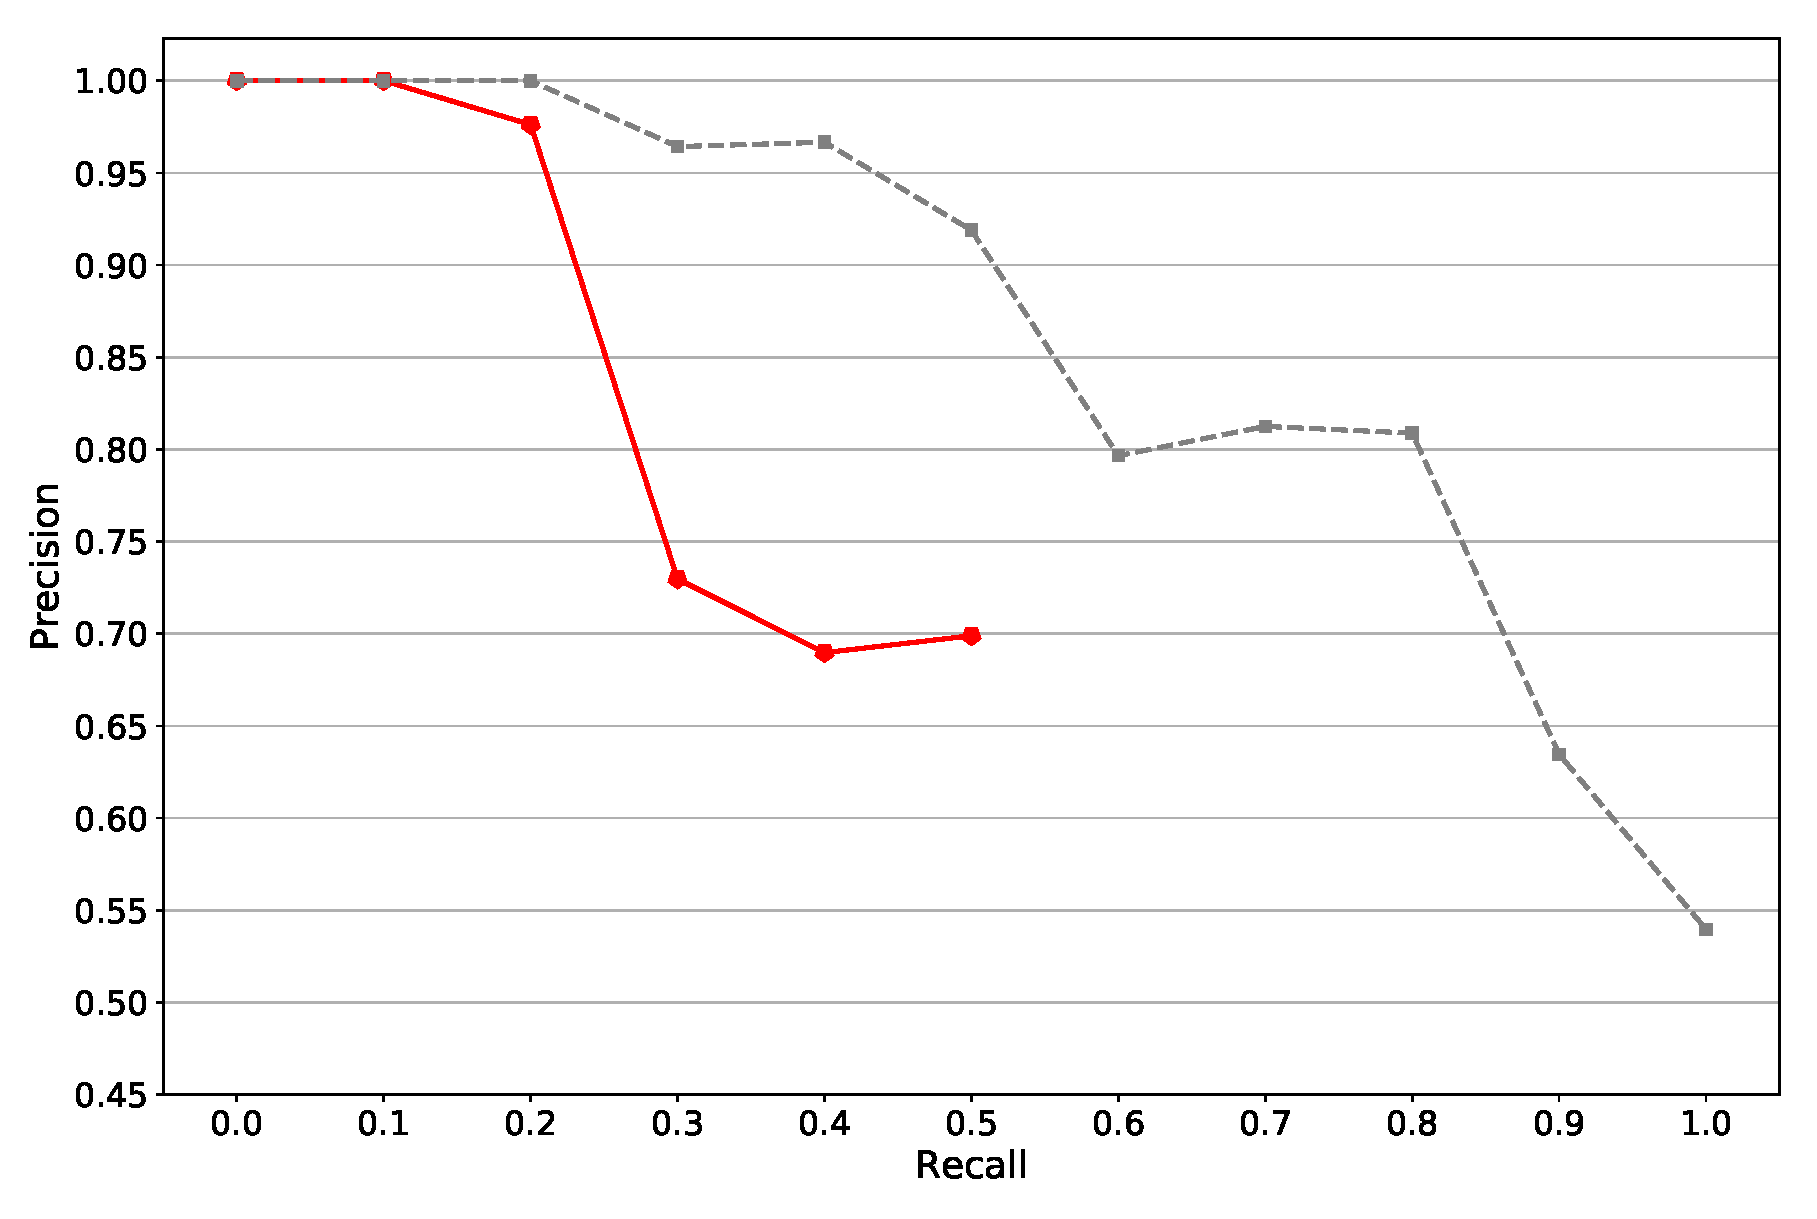
\includegraphics[scale=0.45]{Figures/pr_macro_micro_example.eps}
		\caption{Open-set Macro (Red line) and Micro (grey line) Precision Recall Curves of confusion matrix in table \ref{chap:eval_methods:tbl:multi_confusion}}
		\label{chap:eval_methods:fig:prc_macro}
	\end{center}
\end{figure}

The two curves yielding from this calculations, micro and macro PRC are shown in figure \ref{chap:eval_methods:fig:prc_macro}. Clearly, the micro-PRC is misleading compare to the macro-PRC and the results of table \ref{chap:eval_methods:tbl:macro_vs_micro}. 

The micro-P and micro-R is measures (in table \ref{chap:eval_methods:tbl:macro_vs_micro}) are leading to the conclusion of a low performance algorithm, especially for the recall score. On the contrary the micro-PRC is leading to the conclusion of a high performance algorithm, which we know that it is not true, form the confusion matrix of \ref{chap:eval_methods:tbl:multi_confusion}.

To compensate the potentially unbalanced distribution of web pages over the genres, the macro-averaged precision and recall measures is used. In more detail, in this thesis a modified version of precision and recall is used, for open-set classification tasks proposed by \parencite{mendesjunior2016}. This modification calculates precision and recall only for the known classes (available in the training phase) while the unknown samples (belonging to classes not available during training) affect false positives and false negatives.

The problem of the misleading micro-PRC is cased by the presence of the outages, depicted in the first row, in the confusion matrix \ref{chap:eval_methods:tbl:multi_confusion}. Particularly, as shown in table \ref{chap:eval_methods:tbl:prc} and the rows 10 and 13, the micro-PRC calculation is considering the rejected incorrect predicted and it is including them in the prediction. Thus these predictions are not calculated in the precision equation \ref{chap:eval_methods:eq:precision}. These predictions are just decreasing the micro-R. Consequently, the curve is overestimating the performance of the algorithm.

On the contrary the macro-PRC is closer to the macro prediction and recall. Particularly it is show that the curve stops near the $0.5$ values which is equal to the macro-R. Moreover, macro-precision is high yet drops significantly due to the $0.69$. The PRC is giving the same evaluation performance with the table's \ref{chap:eval_methods:tbl:macro_vs_micro} scores per class and macro-scores. That is, the algorithm is having really good performance for some classes and really bad for some other.

However, due to the certainty ranking we can see more insight related to the algorithms performance. Particularly, we can see some irregular drops in the curves (both macro and micro) also the slope of the first recall level to the second and third is very small and then drops from the near perfect predictions to the $0.73$ precision etc. Also, the curve it stops at $0.5$ recall level.

These, PRC 'irregular' properties are only meet at the open-set algorithms because of the rejection factor. In table \ref{chap:eval_methods:tbl:prc} the algorithms of the precision in rows 10 and 13, seems to have $0.60$ certainty factor which is almost as high as its correct predictions. These predictions are casing high fluctuations in the PRC which are regularized because the 11-recall level average normalization is applied on top. 

The 11-Recall level average normalization is a standardized evaluation in the text mining domain and it is also used in this thesis. the Precision-Recall curve is calculated in 11-standard recall levels $[0,0.1,...,1.0]$. Precision values are interpolated based on the following formula of equation \ref{chap:eval_methods:eq:11recall_level}.

\begin{equation}\label{chap:eval_methods:eq:11recall_level}
	P(r_j)=max_{r_j \leqslant r \leqslant r_{j+1}}(P(r))
\end{equation}

\noindent
where $P(r_j)$ is the precision at $r_j$ standard recall level.


\section{Area Under the Curve (AUC)}\label{chap:eval_methods:sec:closed_set_classification} 

To find parameter settings that obtain optimal evaluation performances we use 2 scalar measures, the Area Under the Precision-Recall Curve (AUC)and $F_{1}$. We will show that the appropriate selection of the optimization measure is highly significant in the presence of noise.


\section{Re-defining the Open Space Risk}\label{chap:eval_methods:sec:open_space_risk} 

The open space risk in \parencite{scheirer2013toward} is originally defined as in eq. \ref{chap:eval_methods:eq:the_original_open_space_risk}

\begin{equation}\label{chap:eval_methods:eq:the_original_open_space_risk}
	R_{o}(f) = \frac{\int_{o} f_{y}(x) dx}{\int{S_{o}}  f_{y}(x) dx}
\end{equation}

\noindent
where $R_{o}(.)$ is the open-space risk function and $f_{y}(x)  \in \{0, 1\}$ is the classification function of class $y$, where $1$ is for recognizing its class and $0$ when not. $S_{o}$ is the large hyper-sphere where all the positive training data points and the \textit{positive open space area} $O$. 

The original formulation of the eq. \ref{chap:eval_methods:eq:the_original_open_space_risk} $O$ area cannot be constrained by any means. The only information we are getting is the farther form the training date we go the risk of miss-classification is increasing One method to constrain the problem is by using the center of the positively labeled training data and defining a radios $r_{o}$ where it will reduce the open space area based on the positively labeled empirically observations. Then the $O$ is defined by the equation eq. \ref{chap:eval_methods:eq:openspace_spherical_constrained}

\begin{equation}\label{chap:eval_methods:eq:openspace_spherical_constrained}
	O = S_{o} - B_{r_{y}}(C_{y})
\end{equation}

\noindent
where $B_{r_{y}}(.)$ is the function which defines the area of radius $r_{y}$ of the $C_{y}$ class defined by its training data \parencite{fei2016breaking}.

\section{Openness test}\label{chap:eval_methods:sec:open_space_risk}

In \parencite{scheirer2013toward} work in image processing, the \textit{openness measure} is introduced, as shown in eq. \ref{chap:eval_methods:eq:openness}. The openness measure indicates properties of an open-set classification task by taking into account the number of \textit{training classes}, i.e. the known labels used in the training phase and the number of \textit{testing classes}, i.e., the labels, both known and unknown, used in the testing phase.

\begin{equation}\label{chap:eval_methods:eq:openness}
	openness=1-\sqrt{\frac{ | Training Classes | }{ |Testing Classes | }}
\end{equation}

When openness is $0.0$, it is essentially a closed-set task, that is the training and testing classes are the same or there is no noise. When openness reaches $1.0$ this means that the known classes are far less than the unknown classes, that is the amount of noise is especially high. Therefore, by varying the openness level we can study the performance of WGI models in different conditions.

Note that the openness measure can only be applied to corpora where all available documents have been labeled with genre information. In other words, we have to know the genre labels of the pages that form the noise (i.e. structured noise). Thus, it cannot be applied to SANTINIS corpus where the web pages taken from the SPIRIT collection are unclassified (i.e., unstructured noise). On the other hand, the SANTINIS corpus provides the opportunity to examine WGI performance when all documents not belonging to the known labels are grouped into one single (highly heterogeneous) class.


\section{Domain Transfer Measure}\label{chap:eval_methods:sec:domain_transfer_measure}

A practical methodology for evaluating a classification/identification ML model in a text-categorization task is the \textit{Domain Transfer Evaluation}. The goal of this evaluation methodology is to measure the generalization of the model when training corpus is rather small and to evaluate how the model would perform in an unknown domain for the same task. 

Particularly for the AGI/WGI with this measure we can evaluate a ML algorithm when for example the model has been trained to identify \textit{News} and \textit{Wiki} genres, however, the available corpus would be only from \textit{Technology products Topics}. Then by testing it on {Sports Topics} we could evaluate the model in such a case when very small corpus is available for training. In addition using this methodology we can evaluate the models behavior depending on the \textit{Features} have been selected for the training, e.g. BOW, POS, Term N-grams etc. 

One can measure the performance, say Accuracy, F1-statistic, Precision-Recall Curve,  Receiver Operating Characteristic (ROC) Curve etc, and then compare the two measures pairwise for every domain combination (e.g. $\{Mobile Phones, Football\}$, etc). However, it would be easier to have measure for all possible combinations training/testing of different domain combinations. 

The measure proposed from \parencite{finn2006learning} and shown in equation \ref{eq:gnr_dom_transit_general} in its generalized form. Originally, this measure was designed for Accuracy measure in mind. However, it can be used for any measure say $F_{1}$-statistic in order to fit in open-set framework and not respected to the closed-set also (Να ελέγξω αν το Accuracy μπορεί να χρησιμοποιηθεί για Open-set). 

\begin{equation} \label{chap:eval_methods:eq:office_doc_ensemble}
	T^{C,F} = \frac{1}{N(N-1)} \sum_{A=1}^{N} \sum_{B, \forall B \neq A}^{N} \left(  \frac{M^{C,F}_{A,B}}{M^{C,F}_{A,A}} \right)
	\end{equation}

	\noindent	
where T is the \textit{Transfer Measure Score}, M is the measure of choice (Accuracy, $F_1$, Precision, Recall, etc), F is the \textit{Feature Set}, and C is the \textit{Genre Class}. 

























%!TeX spellcheck = en-US

%\chapter{Handling the Noise of the Web-Genres}
\chapter{Experimental Analysis of Open-set WGI Methods}

\label{chap:noise}

%----------------------------------------------------------------------------------------

% Define some commands to keep the formatting separated from the content
\newcommand{\keyword}[1]{\textbf{#1}}
\newcommand{\tabhead}[1]{\textbf{#1}}
\newcommand{\code}[1]{\texttt{#1}}
\newcommand{\file}[1]{\texttt{\bfseries#1}}
\newcommand{\option}[1]{\texttt{\itshape#1}}

%----------------------------------------------------------------------------------------

\section{Introduction}\label{chap:noise:sec:intro}

Based on the evaluation framework described in the previous chapter, it is now possible to evaluate the open-set WGI algorithms presented in chapter \ref{chap:openset}. Certainly, any kind of empirical evaluation depends on the dataset that is used for estimating the performance of the examined models. Each dataset has its weaknesses and this might lead to an over-estimation or under-estimation of performance of the examined methods in more realistic conditions. However, what we want to study here is the comparison of performance of different approaches on exactly the same datasets and experimental setup to extract conclusions about the relative improvement in performance of one method with respect to another.

In this thesis, we focus on the effect of noise in open-set WGI approaches. In particular, we want to examine the performance of WGI methods when either unstructured or structured noise is available. The former is a realistic scenario in most WGI applications where it is difficult, if not impossible, to define the genre of a large part of the web. In such cases, it is better to assume that the unknown class comprises any kind of web-pages that do not belong to the known genres. On the other hand, this makes the definition of noise chaotic and extremely heterogeneous. 

The case of structured noise offers the opportunity to study the performance of open-set WGI methods when the heterogeneity of noise can be controlled. The assumption that information about the unknown classes is available (although the classifier has no training examples for these classes) is not unrealistic. For example, an open-set WGI system that aims to recognize news articles should not be distracted by blogs. That is, we know that blogs exist and perhaps comprise the majority of noise in that system but we do not provide training examples for that class.

Among the three open-set WGI methods proposed in this thesis, OCSVM and RFSE are examined in this Chapter while NNDR is thoroughly tested in Chapter \ref{chap:word_embeddings}. The reason for this is that NNDR is especially difficult to be tested in conditions of structured noise, especially when limited known classes are available since a part of known classes have to be used for estimating the open space risk. Therefore, NNDR is only tested with unstructured noise.

The estimation of performance of WGI methods also depends on the applications they are going to be used. Some applications require high precision (e.g., ranking genre-based search results). On the other hand, it is rather unusual to aim for high recall with the cost of reducing precision in WGI-related applications. The experimental analysis should also reflect these facts.

Another crucial issue is the representation of web-pages. As already explained in chapter \ref{chap:openset} the dimensionality of representation, the existence of irrelevant and redundant features can severely harm the performance of certain open-set WGI methods. Therefore, it is important to study how different text representation schemes, especially the ones that were found to be the more reliable ones in previous WGI studies, affect the performance of the examined methods. 

In the remaining of this chapter, we first describe the datasets used in this study and the experimental setup. Then, we present the experimetntal results in open-set WGI when either unstructured noise or structured noise is available. Finally, we summarize the drawn conclusions.

\section{Corpora}\label{chap:noise:sec:corpora}
In this paper we study the performance of the open-set classification models on the WGI task. In particular, the two open-set algorithms described above are analytically tested on benchmark corpora. In particular, our experiments are based on the following corpora already used in previous work in WGI \parencite{meyer2004genre,santini2007automatic,kanaris2009learning}:

\begin{enumerate}
	\item \textit{SANTINIS} \parencite{mehler2010genres_on_web}: This is a corpus comprising 1,400 English web pages evenly distributed into 7 genres as well as 80 BBC web pages evenly categorized into 4 additional genres. In addition, it comprises a random selection of 1,000 English web pages taken from the SPIRIT corpus \parencite{joho2004spirit}. The latter can be viewed as noise in this corpus. Details are given in table \ref{chap:noise:tbl:genre_tags}.
	\item \textit{KI-04} \parencite{meyer2004genre}: This is a collection of 1,205 English web pages unevenly categorized into 8 genres. Details can be seen in table \ref{chap:noise:tbl:genre_tags}.
\end{enumerate}


\section{Experimental Setup}\label{chap:noise:sec:experimental_setup}

The text representation features used in this thesis are based exclusively on textual information from web pages excluding any structural information, URLs, etc. This does not mean that we consider other kinds of information (e.g., HTML-based features, URL-based features etc.) as less important in WGI. However, information coming from the text itself is less likely to be affected by technology-related choices that can be easily altered through time. By focusing on the text of the web pages we ensure that the drawn conclusions are more reliable and long lasting.

Based on the good results reported in \parencite{sharoff2010web,kanaris2009learning,Asheghi2015} as well as some preliminary experiments, the following document representation schemes are examined: 

\begin{itemize}
    \item Character 4-grams (C4G)
    \item Word unigrams (W1G)
    \item Word 3-grams (W3G)
    \item Part-of-speech 3-grams (POS3G)
\end{itemize}

The Stanford POS tagger has been used for POS3G creation. We use the Term-Frequency (TF) weighting scheme and the feature space is defined by a \textit{Vocabulary} which is extracted based on the terms appearing at training set only. There is no pre-processing of textual data (e.g., stop word removal, stemming etc.) since in style-based text categorization tasks these processes remove significant stylistic information \parencite{stamatatos2009survey}.

Each open-set WGI method has some hyper-parameters to be tuned. In order to extract the best possible parameter settings for each classification method we apply grid-search over the space of all parameter value combinations. This is not the most sophisticated approach but ensures that the extracted parameter values will fine-tune the model for the specific dataset.

As concerns OCSVM method, two parameters have to be tuned: the number of features $F$ and $\nu$. For the former, we used $F=$\{1k, 5k, 10k, 50k, 90k\}, of most frequent terms of the vocabulary. Following the reports of previous studies \parencite{scholkopf1999estimating} and some preliminary experiments, we examined $\nu$=\{0.05, 0.07, 0.1, 0.15, 0.17, 0.3, 0.5, 0.7, 0.9\}. In comparison to \parencite{pritsos2013open}, this set of parameter values is more extended. 

With respect to RFSE, four parameters should be set: the vocabulary size $F$, the number of features used in each iteration $fs$, the number of iterations \textit{I}, and the threshold $\sigma$. We examined $F$=\{5k, 10k, 50k, 100k\}, $fs$=\{1k, 5k, 10k, 50k, 90k\}, \textit{I}=\{10, 50, 100\} (following the suggestion in \parencite{koppel2011authorship} that more than 100 iterations does not improve significantly the results) and $\sigma$\textit{=\{0.5, 0.7, 0.9\}} (based on some preliminary tests). Additionally, in this thesis we test three document similarity measures used in RFSE approach: cosine similarity, MinMax similarity, and Combo (as defined in Section \ref{chap:openset:sec:RFSE_Description}). 

%Finally, for the NNDR approach, there are two parameters to be tuned: $lambda$ and DRT. The considered values are: $\lambda =\{0.2, 0.5, 0.7\}$, $DRT=\{0.4, 0.6, 0.8, 0.9\}$. 

%\textcolor{red}{WHAT ABOUT $P_1$ and $P_2$ (in the estimation of DRT)}

\begin{table}[t]
\center
\begin{tabular}{|l|l|l|l|}
\hline
\multicolumn{2}{|c|}{SANTINIS} & \multicolumn{2}{c|}{KI-04}\tabularnewline
\hline
\multicolumn{1}{|c|}{Genre} & \multicolumn{1}{c|}{Pages} & \multicolumn{1}{c|}{Genre} & \multicolumn{1}{c|}{Pages}\tabularnewline
\hline
\multicolumn{1}{|l|}{Blog} & \multicolumn{1}{c|}{200} & \multicolumn{1}{l|}{Article} & \multicolumn{1}{c|}{127}\tabularnewline
\multicolumn{1}{|l|}{Eshop} & \multicolumn{1}{c|}{200} & \multicolumn{1}{l|}{Discussion} & \multicolumn{1}{c|}{127}\tabularnewline
\multicolumn{1}{|l|}{FAQ} & \multicolumn{1}{c|}{200} & \multicolumn{1}{l|}{Download} & \multicolumn{1}{c|}{152}\tabularnewline
\multicolumn{1}{|l|}{Frontpage} & \multicolumn{1}{c|}{200} & \multicolumn{1}{l|}{Help} & \multicolumn{1}{c|}{140}\tabularnewline
\multicolumn{1}{|l|}{Listing} & \multicolumn{1}{c|}{200} & \multicolumn{1}{l|}{Link Collection} & \multicolumn{1}{c|}{208}\tabularnewline
\multicolumn{1}{|l|}{Personal Home Page} & \multicolumn{1}{c|}{200} & \multicolumn{1}{l|}{Portrayal-Non Private} & \multicolumn{1}{c|}{179}\tabularnewline
\multicolumn{1}{|l|}{Search Page} & \multicolumn{1}{c|}{200} & \multicolumn{1}{l|}{Portrayal- Private} & \multicolumn{1}{c|}{131}\tabularnewline
\multicolumn{1}{|l|}{DIY Mini Guide (BBC)} & \multicolumn{1}{c|}{20} & \multicolumn{1}{l|}{Shop} & \multicolumn{1}{c|}{175}\tabularnewline
\multicolumn{1}{|l|}{Editorial (BBC)} & \multicolumn{1}{c|}{20} &  & \tabularnewline
\multicolumn{1}{|l|}{Features (BBC)} & \multicolumn{1}{c|}{20} &  & \tabularnewline
\multicolumn{1}{|l|}{Short Bio (BBC)} & \multicolumn{1}{c|}{20} &  & \tabularnewline
\multicolumn{1}{|l|}{Noise (Spirit1000)} & \multicolumn{1}{c|}{1000} &  & \tabularnewline
\hline
\end{tabular}
\caption {Corpora descriptions and amount of pages per genre.}
\label{chap:noise:tbl:genre_tags}
\end{table}


\section{WGI with Unstructured Noise}\label{chap:noise:sec:WGI_noise}

The two open-set algorithms RFSE and OCSVME, describe in sections \ref{chap:openset:sec:alg:OCSVM_Ensemble} and \ref{chap:openset:sec:alg:RFS-Ensemble}, are initially tested on SANTINIS corpus which as explained above is an Unstructured Noise, samples corpus.   

In the training phase, only the 11 known genres are considered. In the testing phase, the noise pages coming from the SPIRIT corpus are also used. It is important to be noted that information about the true genre of these pages is not available. The 10-fold cross validation is performed where in each fold the full set of 1,000 pages of noise is included. This evaluation strategy is giving a more realistic evaluation framework since the size of the noise is much greater than the size of any genre included in the given palette.

Figures \ref{chap:noise:fig:MacroPRC_OCSVME_W3G_W1G_C4G_OPTIMAL_SANTINIS} and \ref{chap:noise:fig:MacroPRC_RFSE_W3G_W1G_C4G_OPTIMAL_SANTINIS} depict the Precision-Recall curves (PRC) of OCSVM and RFSE models, respectively. For each model and each one of the three document representations, the parameters that maximize performance with respect to the $F_{1}$-measure are used. Remember from section \ref{chap:eval_methods:sec:roc_prc} whenever recall does not reach 1.0 this means that some pages belonging to known classes were classified as unknown. 

In all cases, RFSE outperforms OCSVM. Moreover, for both methods, W3G seems to be the best feature type for this corpus, followed by C4G. OCSVM performance is only comparable with RFSE when W3G is used.

\hfill \break


\begin{figure}[t]
	\begin{center}
    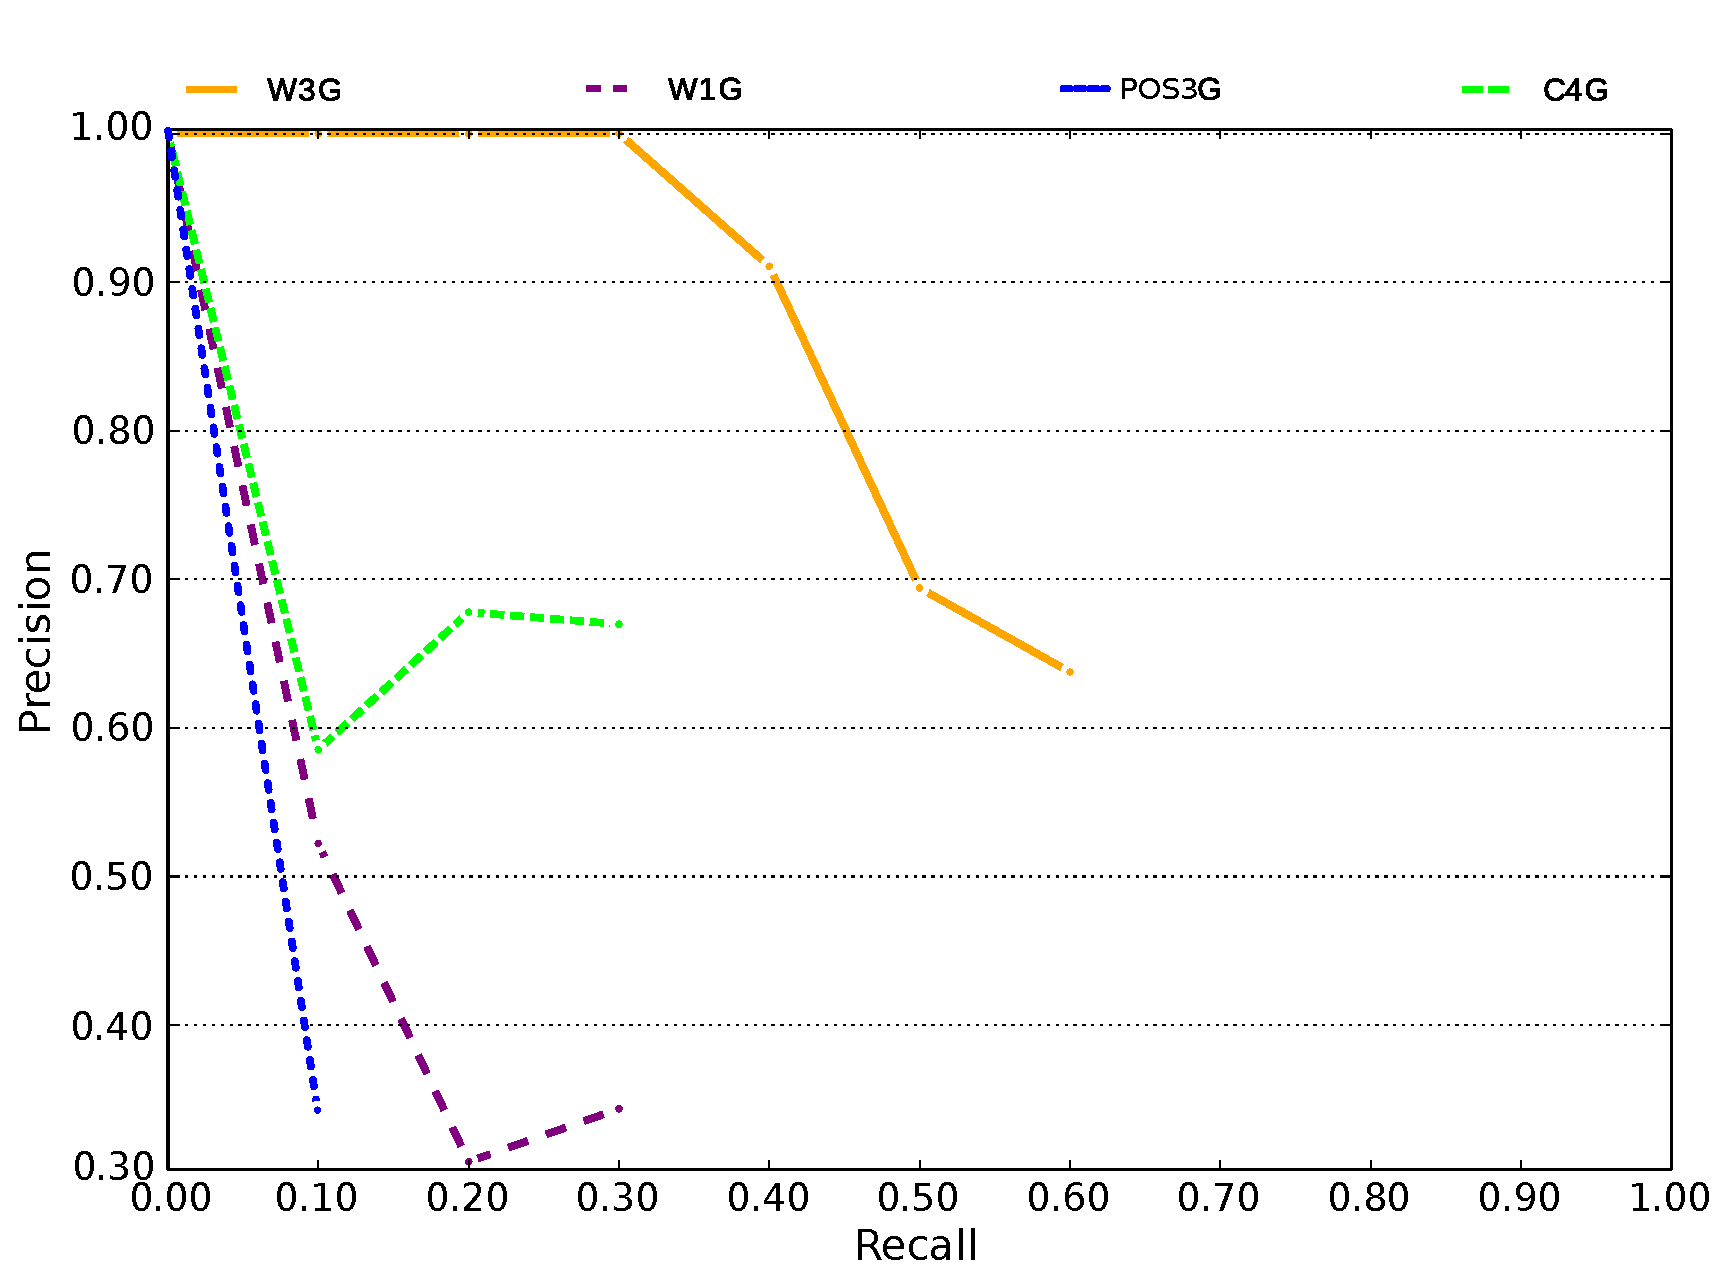
\includegraphics[scale=0.45]{Figures/OCSME_Best_per_DocRep.eps}
	\caption{Precision-Recall Curves of OCSVM models on SANTINIS corpus using W1G, W3G, and C4G features.}
	\label{chap:noise:fig:MacroPRC_OCSVME_W3G_W1G_C4G_OPTIMAL_SANTINIS}
	\end{center}
%\end{figure}

%\begin{figure}[t]
	\begin{center}
    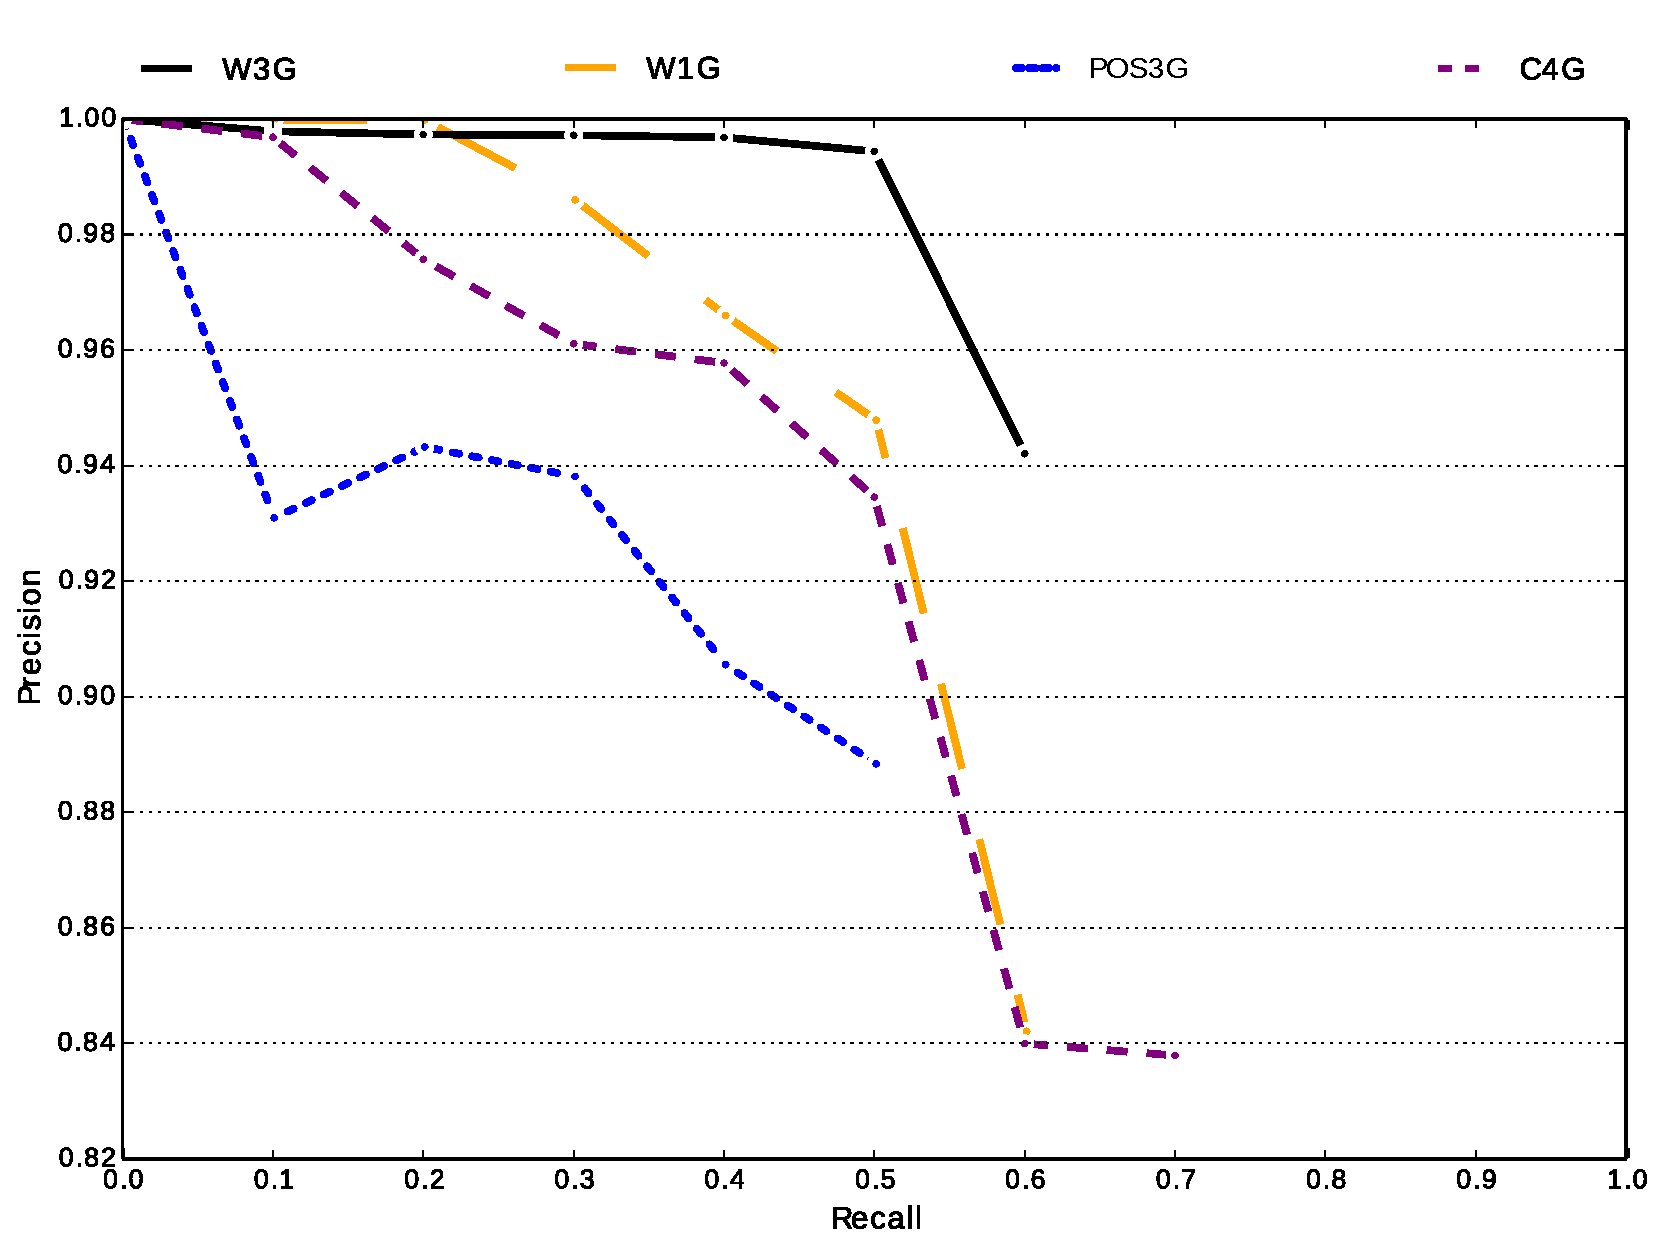
\includegraphics[scale=0.45]{Figures/RFSE_Best_per_DocRep.eps}
	\caption{Precision-Recall Curves of RFSE models on SANTINIS corpus using W1G, W3G, and C4G features.}
	\label{chap:noise:fig:MacroPRC_RFSE_W3G_W1G_C4G_OPTIMAL_SANTINIS}
	\end{center}
\end{figure}

The performance of the open-set WGI methods are further explored by selecting parameter settings with different optimization criteria. Tables \ref{chap:noise:tbl:OCSVME_SANTINIS} and \ref{chap:noise:tbl:RFSE_SANTINIS} show the combination of parameters that optimize performance of OCSVM and RFSE based on AUC, $F_{1}$ and $F_{0.5}$. 

In the tables \ref{chap:noise:tbl:OCSVME_SANTINIS} and \ref{chap:noise:tbl:RFSE_SANTINIS} the values are presented, of all three performance measures where, for every row, one of them is maximized. It is clear that the performance in all cases is maximized when W3G document representation is used. In previous studies based on a closed-set framework, C4G was the document type of features to maximize performance \parencite{Sharroff2010}. This indicates that contextual and content information is important for this corpus \parencite{Asheghi2015}.

In addition, in almost all cases, RFSE models are far more effective than OCSVM. Another important conclusion is that the optimization criterion plays a crucial role for the properties of the model especially for RFSE. When AUC is maximized, recall is favored. On the other hand, while $F_{1}$ is maximized, precision is substantially increased. Fig. \ref{chap:noise:fig:MacroPRC_RFSE_OCSVME_SANTINIS} shows the performance of OCSVM and RFSE models when AUC and $F_{1}$ criteria are used to select parameter settings. As can be seen, the RFSE model based on $F_{1}$ maximization avoids to make wrong decisions and leaves a large number of web pages unclassified. On the other hand, the model optimized by AUC prefers to make a lot of errors in order to recognize more web pages of known genres. OCSVM models seem not significantly affected. Note that choosing between WGI models that prefers precision over recall and vice versa is an application-specific task.



\begin{figure}[t]
\begin{center}
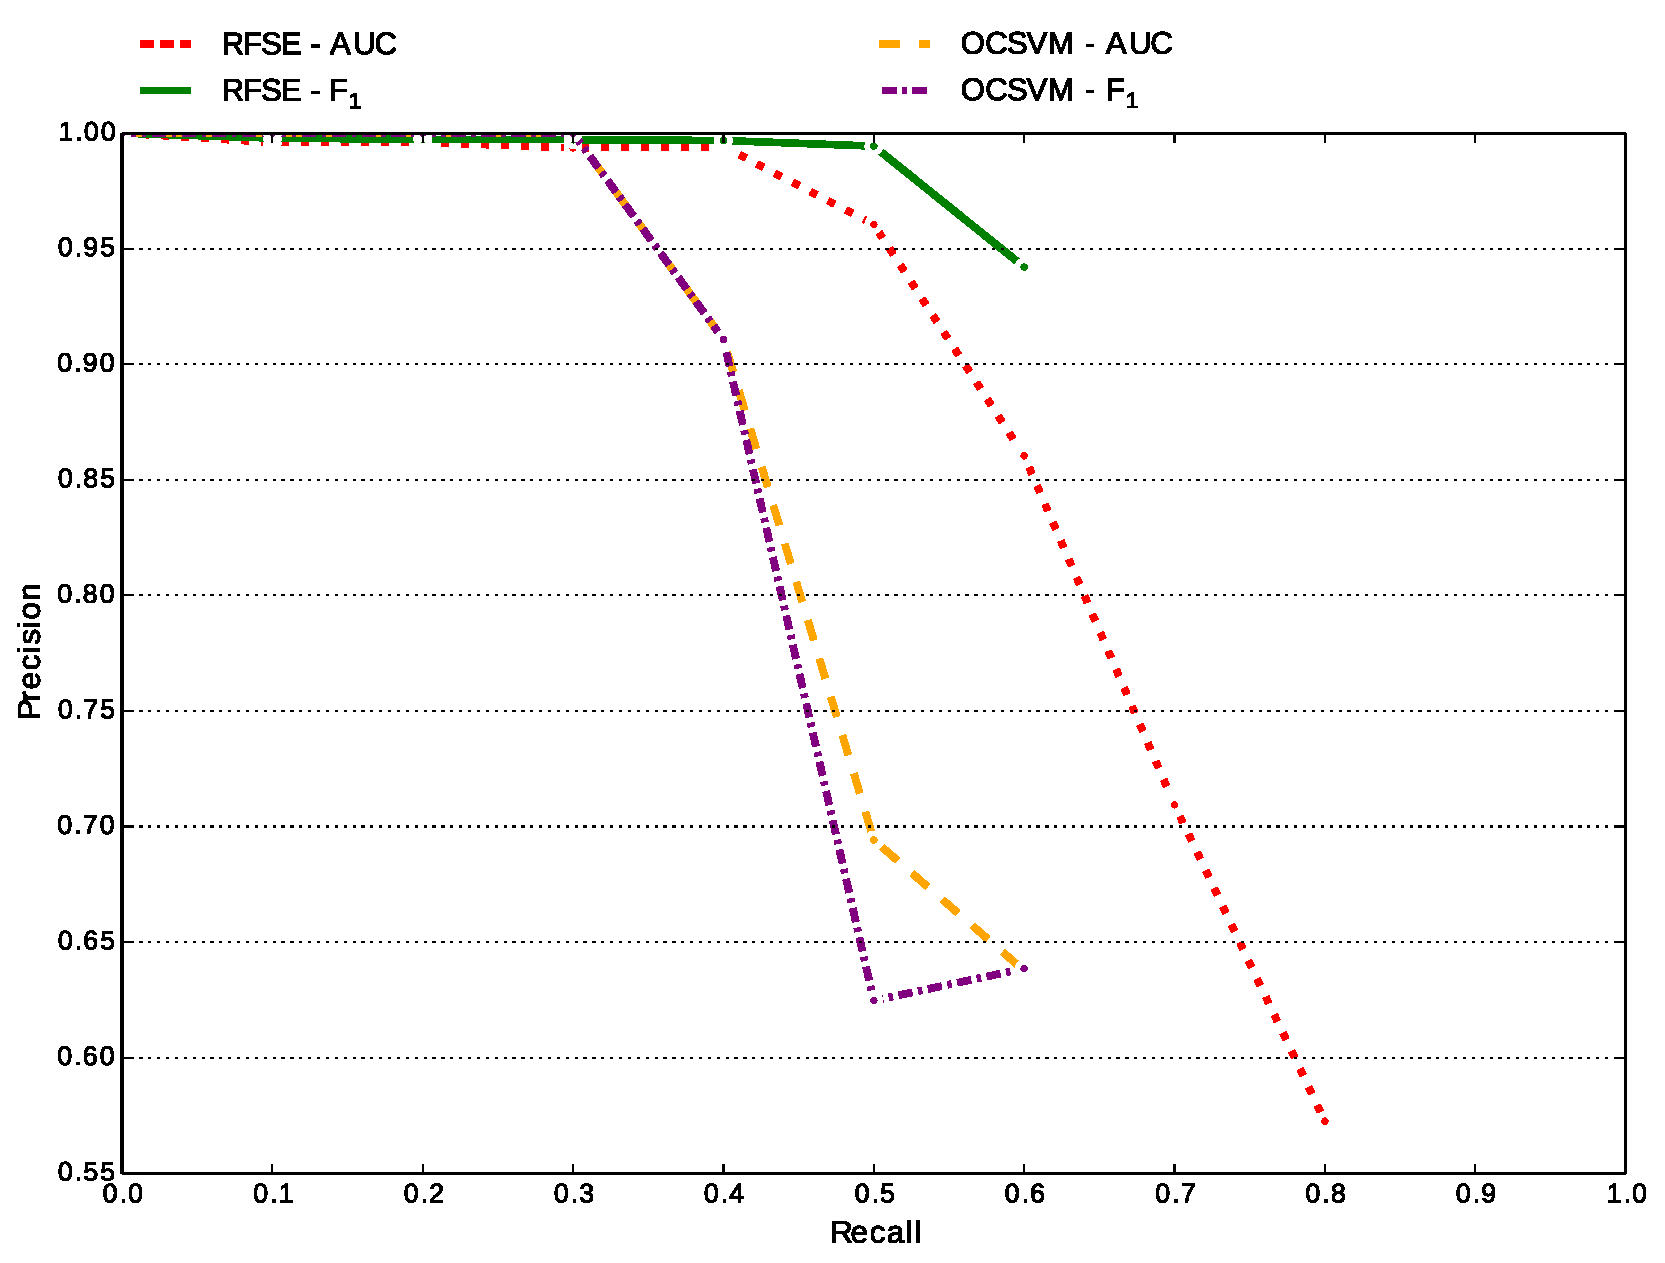
\includegraphics[scale=0.45]{Figures/MacroPRC11AVG_RFSE_OCSVME_SANTINIS_2.eps}
\caption{Precision-Recall Curves of OCSVM and RFSE models on SANTINIS corpus optimized either by AUC or $F_{1}$.}\label{chap:noise:fig:MacroPRC_RFSE_OCSVME_SANTINIS}
\end{center}
\end{figure}

% 7Genres
%
%\begin{table}[t]
%\centering

%\pgfplotstableset{
%    create on use/Criterion/.style={ create col/set list={AUC, $F_{1}$, $F_{0.5}$} },
%	columns/DocRep/.style={string type},
%	create on use/DocRep/.style={ create col/set list={W3G, W3G, W3G} },
%	columns/DocRep/.style={string type}
%}

%\pgfplotstabletypeset[
%		fixed,
%		precision=3,
%		col sep=comma,
%		every head row/.style={
%			before row = \toprule,
%			after row=\midrule,
%		},
%		every last row/.style={after row=\bottomrule \\},
%		columns={Criterion, DocRep, 0, 1, 2, 3, 4, 5, 6, 7},
%		columns/Criterion/.style ={string type,column type=c, column name=Optim.},
%        columns/DocRep/.style ={string type,column type=c, column name=Features},
%		columns/0/.style ={column type=c, column name=Voc.},
%		columns/1/.style ={column type=c, column name=\textit{f}},
%		columns/2/.style ={column type=c, column name=$\nu$},
%		columns/3/.style ={column type=c, column name=Prec.},
%		columns/4/.style ={column type=c, column name=Rec.},
%		columns/5/.style ={column type=c, column name=AUC},
%        columns/6/.style ={column type=c, column name=$F_{0.5}$},
%        columns/7/.style ={column type=c, column name=$F_{1}$},
%		]{tables_data/AUC_FStatistics_tables/OCSVME_SANTINIS_Best.csv}
%\caption{Best performing models for OCSVM on SANTINIS corpus.}
%\label{chap:noise:tbl:OCSVME_SANTINIS}

%\end{table}

\begin{table}[t]
	\center
	\caption{Best performing models for OCSVM on SANTINIS corpus.}\label{chap:noise:tbl:OCSVME_SANTINIS}
	\begin{adjustbox}{width=\textwidth}
	\begin{tabular}{c c c c c c c c c c}
		\hline
		Optim. & Features & Voc. & $f$ & $\nu$ & Prec. & Rec. & AUC & $F_{0.5}$ & $F_{1}$ \\
		\hline
		AUC & W3G & 50,000 & 10,000 & 0.07 & 0.630 & 0.643 & 0.542 & 0.633 & 0.636 \\
		$F_{1}$ & W3G & 50,000 & 10,000 & 0.10 & 0.631 & 0.654 & 0.535 & 0.636 & 0.643 \\
		$F_{0.5}$ & W3G & 100,000 & 50,000 & 0.07 & 0.647 & 0.603 & 0.518 & 0.638 & 0.624\\
		\hline
	\end{tabular}
\end{adjustbox}	
\end{table}

% \begin{table}[t]
% \centering
% 
% \pgfplotstableset{
%     create on use/Criterion/.style={ create col/set list={AUC,$F_{1}$,$F_{0.5}$} },
%     columns/DocRep/.style={string type},
% 	create on use/DocRep/.style={ create col/set list={W3G,W3G,W3G} },
% 	columns/DocRep/.style={string type},
%     create on use/SimMeas/.style={ create col/set list={Combo,MinMax,MinMax} },
% 	columns/SimMeas/.style={string type}
% }
% \pgfplotstabletypeset[
% 		fixed,
% 		precision=3,
% 		col sep=comma,
% 		every head row/.style={
% 			before row = \toprule,
% 			after row=\midrule,
% 		},
% 		every last row/.style={after row=\bottomrule \\},
% 		%columns={Criterion, DocRep, SimMeas, 0, 1, 2, 3, 4, 5, 6, 7, 8},
% 		columns={Criterion, DocRep, SimMeas, 0, 1, 2, 3, 4, 5, 6, 8},
%         columns/Criterion/.style ={string type,column type=c, column name=Optim.},
% 		columns/DocRep/.style ={string type,column type=c, column name=Features},
%         columns/SimMeas/.style ={string type,column type=c, column name=Similarity},
% 		columns/0/.style ={column type=c, column name=Voc.},
% 		columns/1/.style ={column type=c, column name=\textit{f}},
% 		columns/2/.style ={column type=c, column name=$\sigma$},
%         columns/3/.style ={column type=c, column name=\textit{I}},
% 		columns/4/.style ={column type=c, column name=Prec.},
% 		columns/5/.style ={column type=c, column name=Rec.},
% 		columns/6/.style ={column type=c, column name=AUC},
%         %columns/7/.style ={column type=c, column name=$F_{0.5}$},
%         columns/8/.style ={column type=c, column name=$F_{1}$},
% 		]{tables_data/AUC_FStatistics_tables/RFSE_SANTINIS_Best.csv}
% \caption{Best performing models for RFSE on SANTINIS corpus.}
% \label{chap:noise:tbl:RFSE_SANTINIS}
% 
% \end{table}


\begin{table}[t]
\center
\caption{Best performing models for RFSE on SANTINIS corpus.}\label{chap:noise:tbl:RFSE_SANTINIS}
\begin{adjustbox}{width=\textwidth}
\begin{tabular}{c c c c c c c c c c c c}
	\hline
	Optim. & Features & Similarity & Voc. & $f$ & $\sigma$ & $I$ & Prec. & Rec. & AUC & $F_{0.5}$ & $F_{1}$ \\
	\hline
	AUC & W3G & Combo & 50,000 & 10,000 & 0.5 & 100 & 0.572 & 0.824 & 0.730 & 0.609 & 0.670\\
	$F_{1}$ & W3G & MinMax & 50,000 & 5,000 & 0.7 & 100 & 0.933 & 0.680 & 0.595  & 0.868 & 0.787\\
	$F_{0.5}$ & W3G & MinMax & 100,000 & 5,000 & 0.9 & 100 & 0.987 & 0.596 & 0.498 & 0.872 & 0.743\\
	\hline
\end{tabular}

\end{adjustbox}	

\end{table}


\section{WGI with Structured Noise}
\label{chap:noise:sec:openness_evaluation}

In this section the RFSE and OCSVME algorithms we describe experiments using a corpus with structured noise. The KI-04 corpus has been used for this set of experiments. 

The experiments are extensively testing the algorithms' noise tolerance in the open-set classification task for different openness levels as explained in section \ref{chap:eval_methods:sec:openness}. In more detail, the openness measure is adopted varying the number of training classes from 7 to 1 while keeping the number of testing classes always the same, at maximum 8. As a result, the openness measure varies from 0.065 to 0.646. 

One extreme refers to the case where only one genre class is unknown while in the other extreme only one genre class is known. In the extreme case of the maximum openness level, the problem is actually reduced to a binary problem of 1-vs-rest. On the contrary, in the extreme case of minimum openness level, the problem is a multi-class classification with only one unknown class which is virtually complete, i.e. contains single genre pages and no other pages that could be considered as noise.

The known classes are randomly selected for each openness level and the experiment are repeated 8 times, where each time performing 10-fold cross-validation. Moreover, to avoid any biased selection of parameter values, the parameter settings found to be optimal for the SANTINIS corpus are used, in section \ref{chap:noise:sec:WGI_noise}.

Figures \ref{chap:noise:fig:OCSVME_openness_test} and \ref{chap:noise:fig:RFSE_openness_test} show the performance ($F_{1}$) of OCSVE and RFSE models using different text representation features for varying openness levels. Standard error bars are also depicted to show the variance of performance for each model. 

RFSE models based on C4G and W1G gradually get worse while openness increasing while W3G models seems to be relatively stable. Surprisingly, the performance of OCSVM seems to improve by increasing openness and this pattern is consistent in all three feature types while C4G seem to be the most effective type. Although, in the maximum openness level the problem is equivalent to the closed-set binary (i.e. 1-vs-rest) classification problem.

\begin{figure}[t]
\begin{center}
    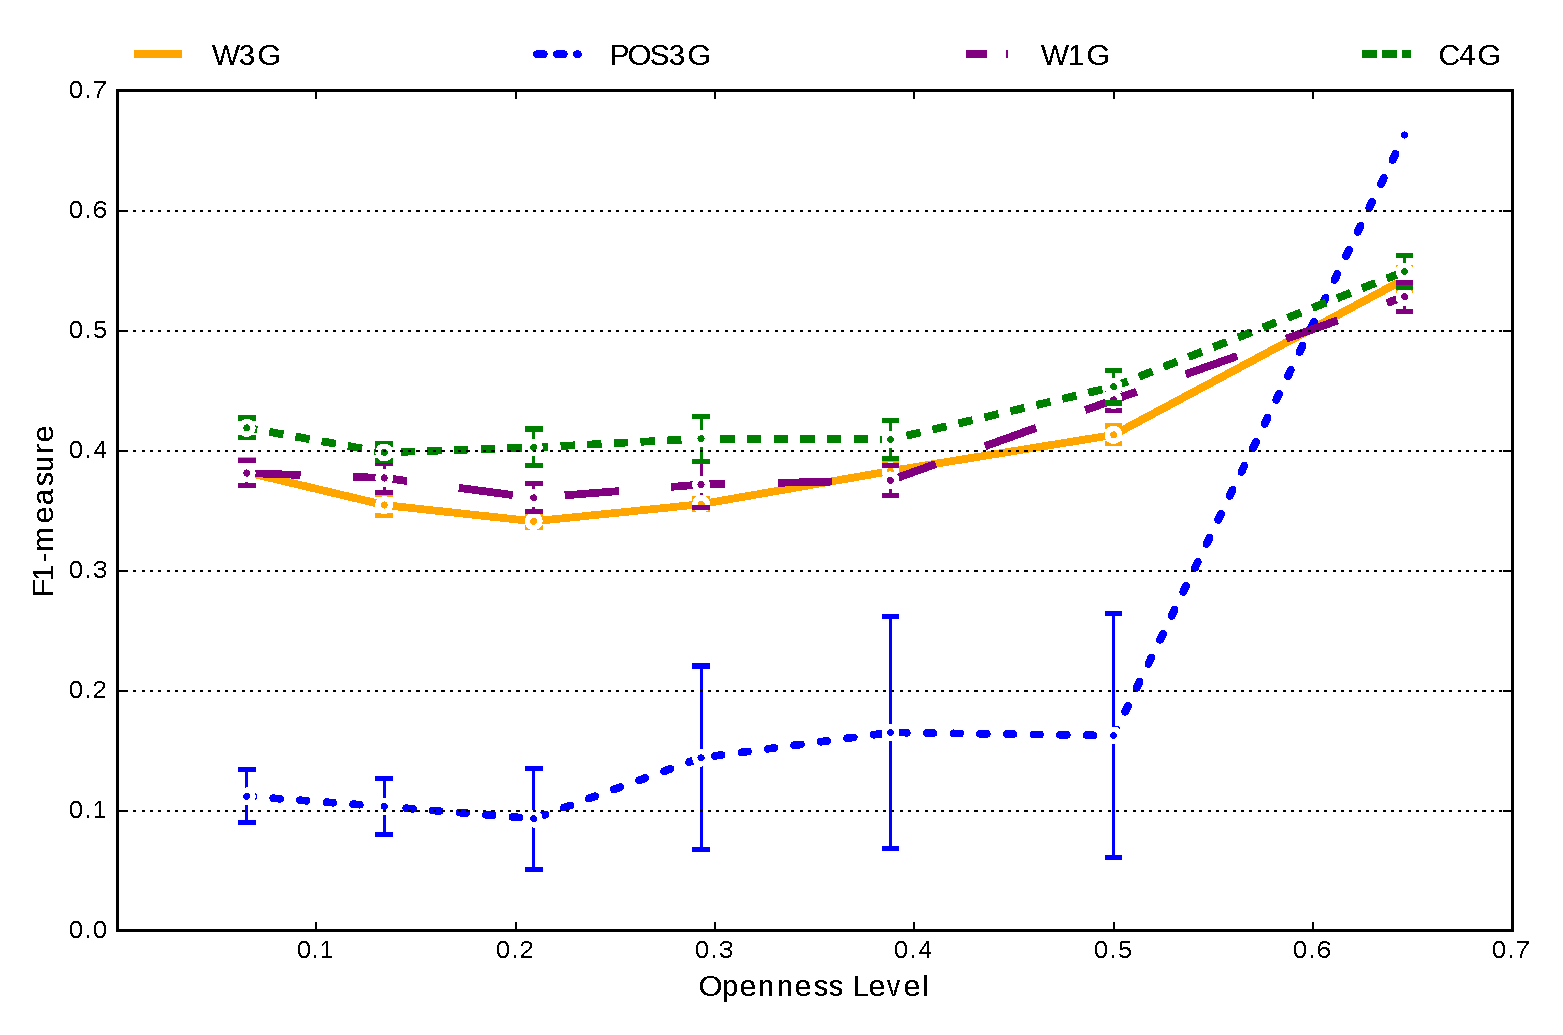
\includegraphics[scale=0.45]{Figures/OCSVME_openness_test_graph.eps}
	\caption{OCSVM performance in varying openness level.}
	\label{chap:noise:fig:OCSVME_openness_test}
\end{center}
\end{figure}

\begin{figure}[t]
\begin{center}
    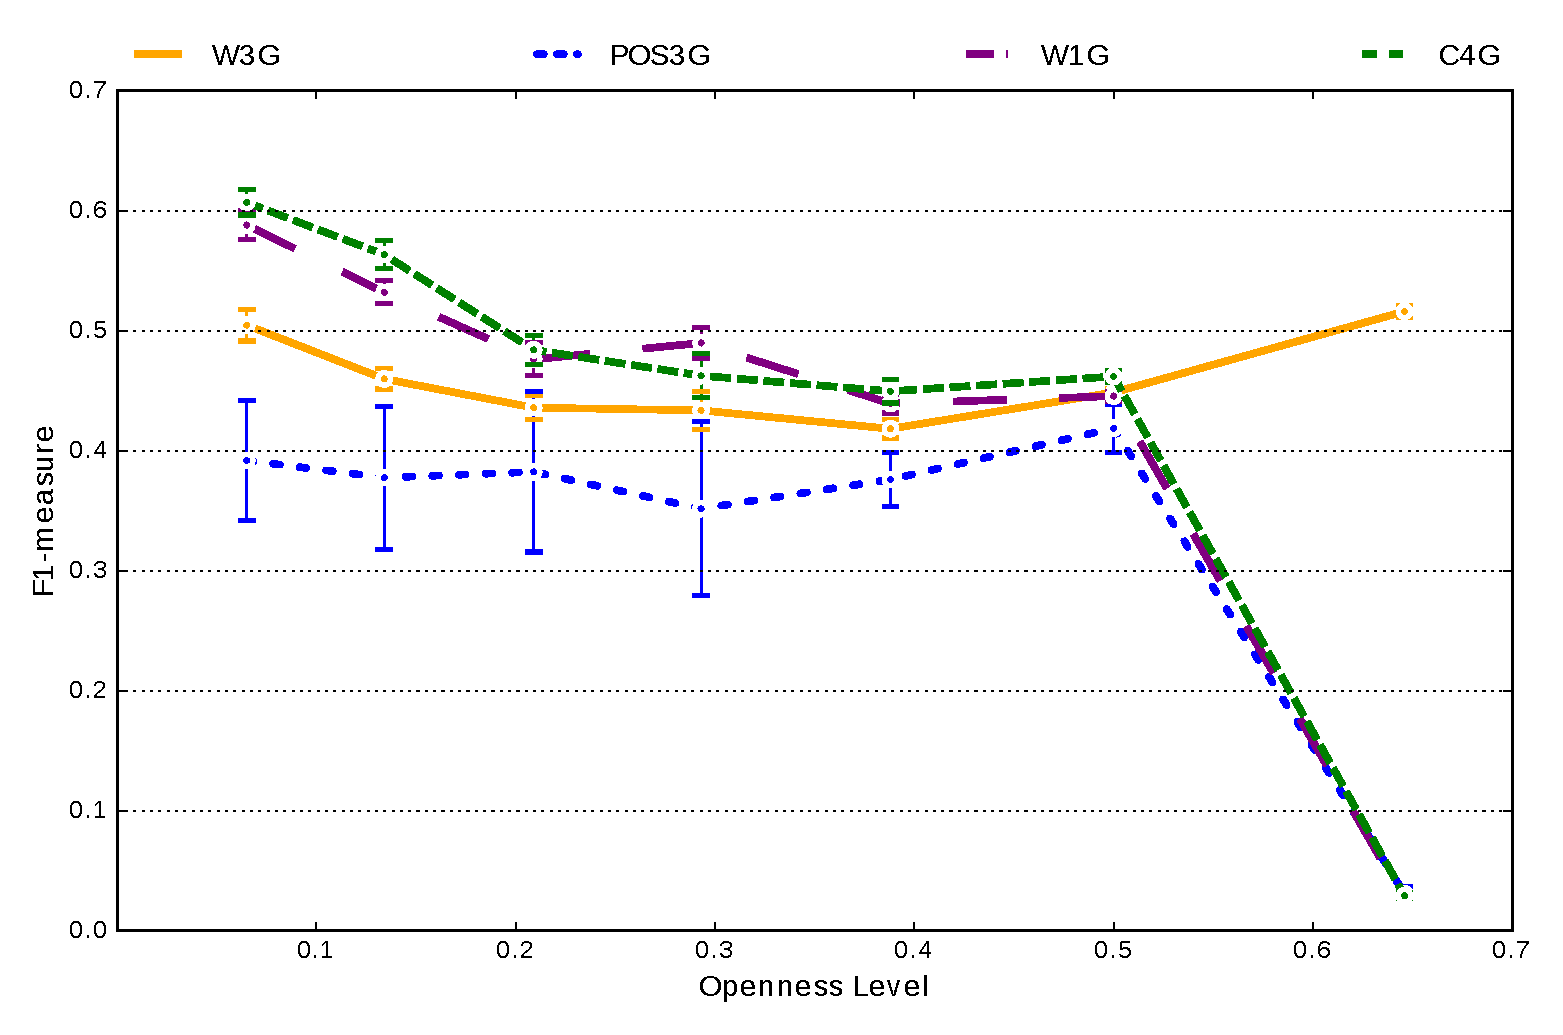
\includegraphics[scale=0.45]{Figures/RFSE_MIX_openness_test_graph.eps}
	\caption{RFSE performance in varying openness level.}
	\label{chap:noise:fig:RFSE_openness_test}
\end{center}
\end{figure}


As it was highlighted in the previous section, according to the properties of the application in which WGI is involved, precision may be more important than recall or vice-versa. In figure \ref{chap:noise:fig:RFSE_precision_focus_openness_test} the macro-precision of RFSE is depicted for W3G, W1G and C4G features. MinMax similarity is used since it increases significantly the performance of RFSE in respect with precision. As concerns text representation, W1G is the best choice when precision is at more importance than recall. On the other hand, W3G features seem to be more stable because the standard error is lower than that of the other features and also the W3G model is not affected too much when openness surpasses $0.5$ (actually it improves).

\begin{figure}[t]
\begin{center}
    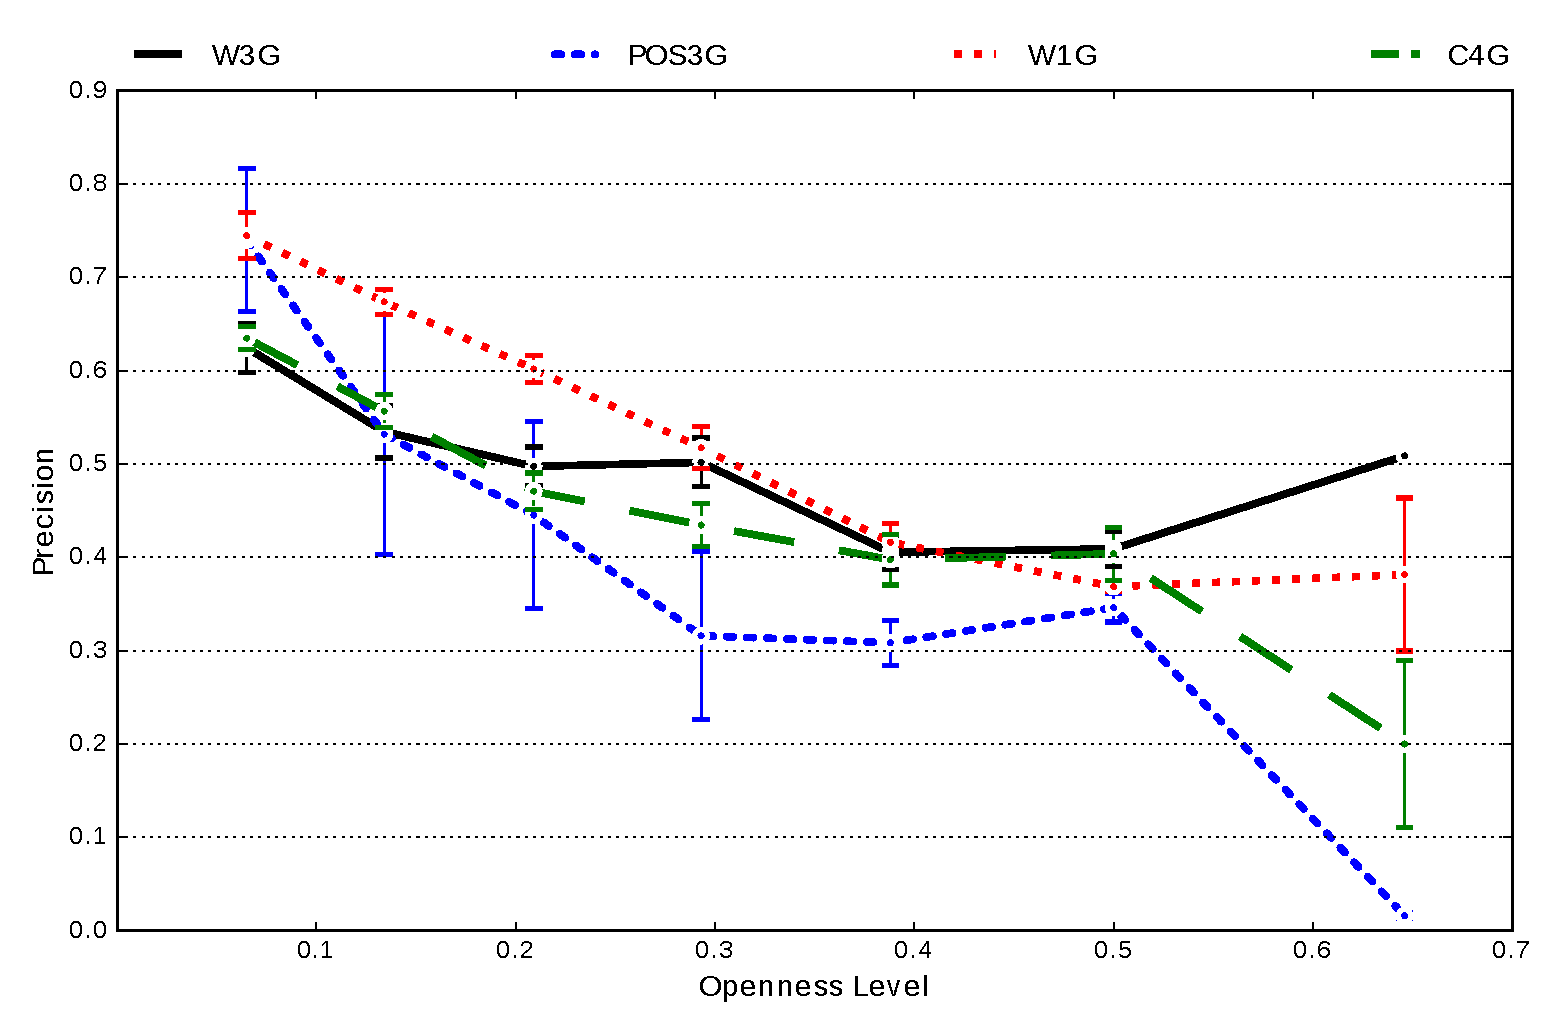
\includegraphics[scale=0.45]{Figures/RFSE_Precision_Focus_openness_test_graph.eps}
	\caption{RFSE precision in varying openness level.}
	\label{chap:noise:fig:RFSE_precision_focus_openness_test}
\end{center}
\end{figure}

In the case of C4G and W1G where the openness level is $0.646$ the standard error in both case is high. Since, this problem is only occurring in the case where the problems has been reduced to binary, it is interesting to see whether it is caused by choice of the document representation or by the choice of the similarity measure.

%In figures \ref{chap:noise:fig:RFSE_MIXvsMinMax_W3GvsC4G_openness_test} the $F_{1}$ measure performance in %the openness test of the RFSE is depicted. In all three cases we see the only with MinMax %similarity the standard error is significantly high especially in the case of $0.646$ openness %level.

Despite OCSVM's improvement when structured noise is used, it can only be competitive to RFSE on a high openness level, where all genre labels but one are considered unknown. This can be better viewed in figure \ref{chap:noise:fig:RFSE_vs_OCSVME_W1G_openness_test} where OCSVM is compared with RFSE models based on MinMax and Combo similarity measures for a varying openness level. These curves correspond to W1G features, so they are not the optimal models. However, they provide a fair comparison between examined methods. As standard error bars indicate, the performance of RFSE models with respect to the $F_{1}$ measure is significantly better than that of OCSVM while openness is less than $0.5$. Beyond that level, OCSVM is significantly better than RFSE models. It should also be noted that Combo measure helps RFSE in while openness is relatively low and MinMax seems to be a better choice when openness increases.

\begin{figure}[t]
\begin{center}
    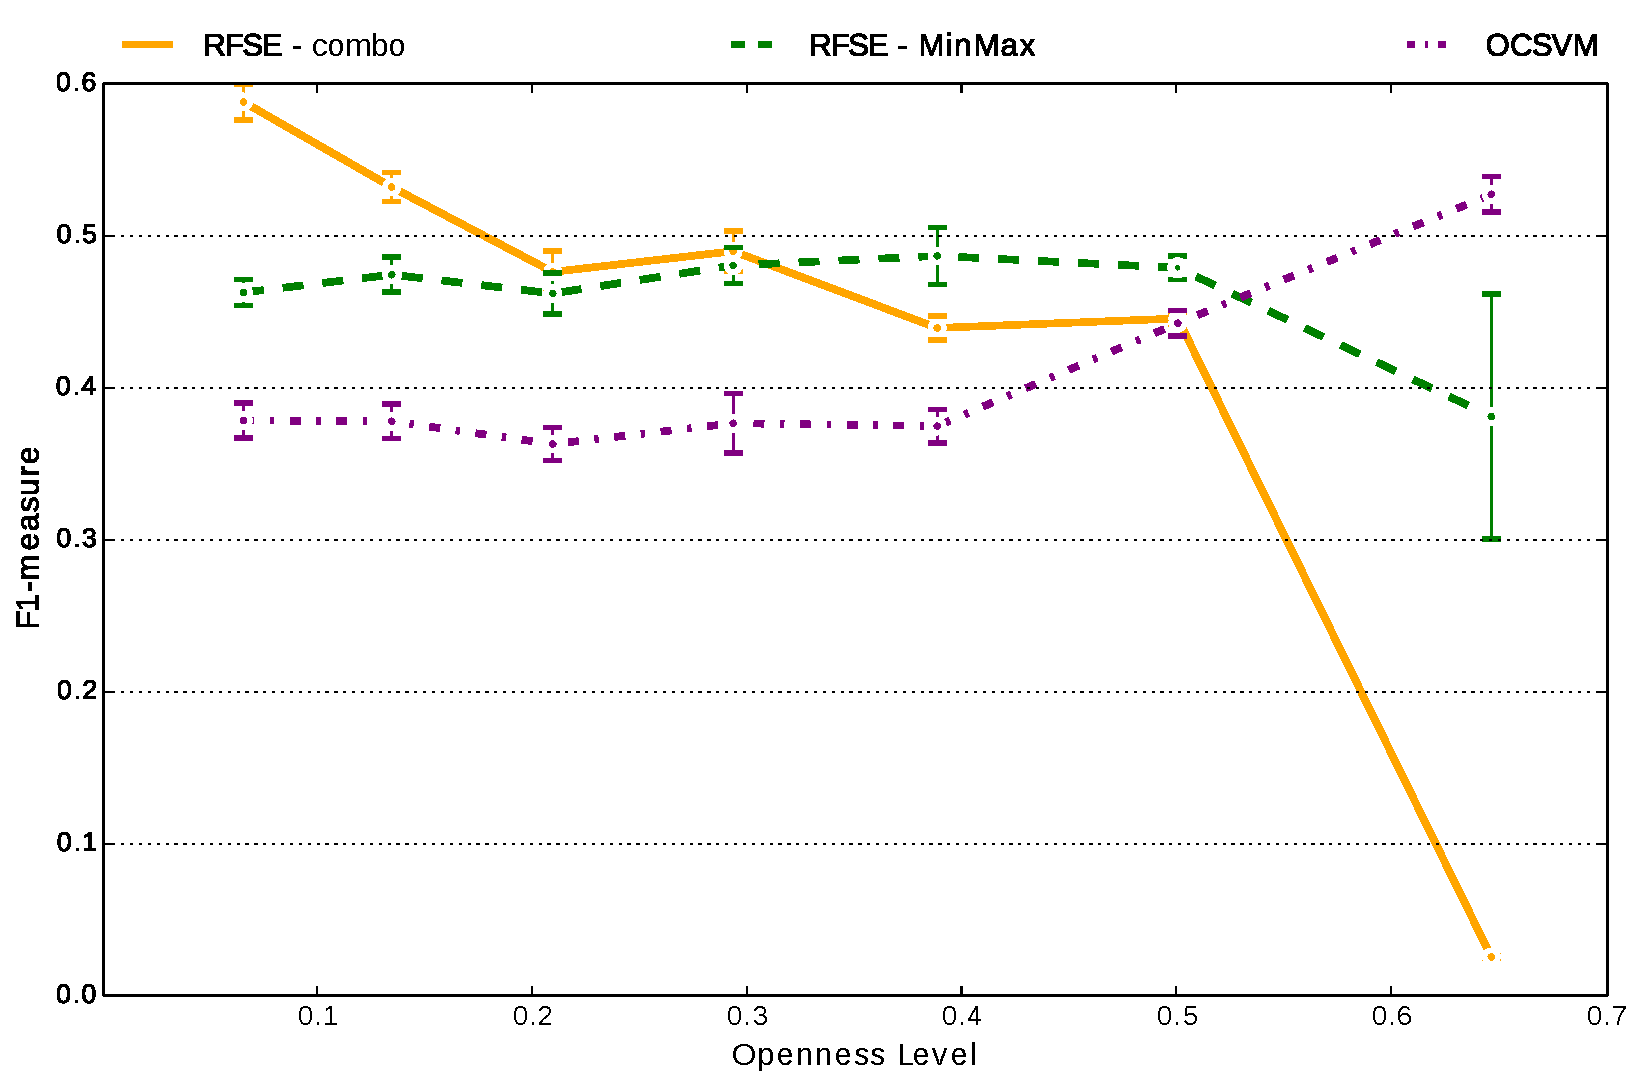
\includegraphics[scale=0.45]{Figures/RFSE_vs_OCSVME_W1G.eps}
	\caption{Comparison of OCSVM and RFSE models based on W1G features in varying Openness levels.}
	\label{chap:noise:fig:RFSE_vs_OCSVME_W1G_openness_test}
\end{center}
\end{figure}

\section{Conclusions}\label{chap:noise:sec:conclusions}

In this chapter it has been presented an experimental study on WGI focusing on open-set evaluation for this task. In contrast to vast majority of previous work in this area, the open-set scenario is adopted which is more realistic for WGI, since it is not feasible to construct a genre palette with all available genres and appropriate samples for each one of them. Moreover, we examined two open-set classification methods and several feature types and similarity measures.

The presented evaluation of open-set WGI covers two basic scenarios. The first is when noise is unstructured, i.e., information about the true genre of pages not belonging to the known genre palette is not available. The second scenario applies when noise is structured, i.e., we actually know the true genre of pages not included in the training classes. For both cases they have been used the proposed appropriate evaluation methodologies for the open-set classification, presented in chapter \ref{chap:eval_methods}.

In almost all examined cases, RFSE models outperformed the corresponding OCSVM models. This verifies previous work findings about the appropriateness of RFSE for WGI \parencite{pritsos2013open}. RFSE is able to provide effective models and additionally it is possible to manage preference on recall or precision, an application-dependent choice, by focusing on optimizing AUC or $F_1$ respectively. On the other hand, OCSVM proved to be the best-performing method in extreme cases when openness is high. Actually, the restrictions of the available corpora did not allow us to examine cases where openness approaches $1.0$. However, it seems that when openness is more than $0.5$ OCSVM outperforms RFSE.

As concerns the feature types, in most of the cases W3G and C4G provided the best results. However, the selection of text representation features is a crucial choice that affects performance and it seems to be corpus-dependent. Another crucial parameter of RFSE is the similarity measure. Among the examined measures, MinMax and its combination with cosine similarity provide the most robust results. The choice of similarity measure correlates with feature types. It seems that the combo measure is more effective than MinMax in low openness conditions.

To enhance the evaluation of WGI models in open-set conditions, we need larger corpora including multiple genre labels. New enhanced open-set WGI methods are needed and they should be evaluated using the proposed paradigm. Otherwise, using an evaluation paradigm more appropriate for closed-set tasks, the performance may be over-estimated.

%!TeX spellcheck = en-US
%\chapter{Word Embedding and Distributional Features of the web-pages and texts}
\chapter{The Usefulness of Distributed Representations in WGI}

\label{chap:word_embeddings}


%----------------------------------------------------------------------------------------

% Define some commands to keep the formatting separated from the content
\newcommand{\keyword}[1]{\textbf{#1}}
\newcommand{\tabhead}[1]{\textbf{#1}}
\newcommand{\code}[1]{\texttt{#1}}
\newcommand{\file}[1]{\texttt{\bfseries#1}}
\newcommand{\option}[1]{\texttt{\itshape#1}}

%----------------------------------------------------------------------------------------

\section{Introduction}\label{chap:word_embeddings:sec:intro}
 
The most traditional text representation scheme in text mining tasks is the Bag-of-Words (BOW) model which is based on individual tokens as features. It is a simplistic approach to quantify textual information assuming independence of the occurrence of individual tokens in documents. The result is a document vector of high dimensionality (i.e., in the order of thousands of features) and sparseness (i.e., only a few non-zero values per document). The BOW model is not able to capture information about the grammar of documents and completely ignores word order. In addition, it is confused by synonym terms since it assumes they are independent. Nevertheless, it provides an easy and quite competitive approach to represent documents (the W1G scheme used in Chapter \ref{chap:noise} is actually based on BOW).

A more elaborate text representation scheme is to consider n-grams of words (e.g., the W3G model used in Chapter \ref{chap:noise}). This would capture information about word sequences, like phrases. This can improve the ablity of the model to represent syntactic information since the context of words is partially taken into account. Nevertheless, the dimensionality of representation is considerably increased when the order of the model ($n$) is high. In addition, the sparseness of the vectors is increased. It is also possible to apply the n-gram approach on the character level or on POS-tag level, as shown in the experiments of Chapter \ref{chap:noise} (i.e., C4G, POS3G). The main assumption that each feature (n-gram) is independent of the other features is still doubtful in such models.

An alternative approach is to use \textit{distributed representations} that attempt to introduce some kind of dependence of each word (or n-gram) on the other words (or n-grams). For example, the words usually encountered in the context of a specific word are more dependent on that word. In addition, different words found in similar context get a higher share of dependence. Distributed representations can be obtained by applying language modeling methods. Especially, the use of neural network language models and the popular word and document \textit{embeddings} introduced in \parentcite{mikolov2013distributed}. 

One main advantage of distributed representations is that they provide compact (i.e., low-dimensional) and dense vectors to quantify syntactic and semantic information in documents. In comparison to regular BOW or n-gram models, distributed features are much less redundant and irrelevant since each such feature captures a combination of information that cannot be specifically determined. Therefore, it seems that open-set WGI methods that are not able to easily handle high-dimensional, sparse vectors with many irrelevant and redundant features would be highly improved by using distributed representations. As already explained in Chapter \ref{chap:openset}, NNDR is an algorithm that, in theory, is vulnerable when it is not combined with appropriate feature sets. The main goal of this Chapter is to examine how the performance of NNDR in WGI tasks is affected when combined with either traditional BOW-like features or distributed features. 

The rest of this chapter is organized as follows. First, the main ideas of distributed representation are presented. Then, the specific distributed features used in this thesis are described. Next, we compare the performance of NNDR using traditional sparse representation schemes with the case dense vectors are used. We also compare these versions of NNDR with OCSVM and RFSE methods and discuss the main conclusions of this study.

\section{Obtaining Distributed Representations}

%The SLM model is defined as the \textit{joint conditional probability distribution} of the next word given the probabilities of previous ones as shown in equation \ref{chap:word_embeddings:eq:slm}

%\begin{equation} \label{chap:word_embeddings:eq:slm}
%	P(w = i) = \prod_{i=1}^{|V|} P(w_{i}|w_{i-k}, ... , w_{i+k})
%\end{equation}
%\noindent
%where $w_{i}$ is the i-th word, and $k$ is for the number of words before or/and and after, writing sub-sequence $w_{i} = (w_{i-k}, w_{i-1}, ... ,w_{i+1}, w_{i+k})$. Note that this model returns a singleton value for a word on the condition of previews or/and next word. This model also can be expanded to have few more words in the conditional probability, usually from 2 up to 4. 

%With this model it can be captured the semantic proximity but it will return zero in the case a sequence have never been met before in the samples. A solution to this problem is the interpolation or smoothness factor that can be applied such as in the \textit{back-off}  model (Katz, 1980 see in bengio2003neural). 

%The model of equation \ref{chap:word_embeddings:eq:slm} can capture the joint probability of word-sequences in terms of feature vectors, however, it cannot capture the correlation of the words in terms of semantics. Models like LSI or LDA are methodologies also been tested in IR and NLP for capturing the semantics in the context of the n-gram based SLM. 

One way to obtain a low-dimensional and dense representation of documents is the use of topic modeling. Topic modeling methods attempt to group terms according to their co-occurrence in documents. They provide a new feature space (composed by latent topics) of pre-defined dimensionality. One popular topic modeling approach is \textit{Latent Semantic Analysis}, a linear algebraic method that transforms a high-dimensional and sparse representation to a low-dimensional and dense one applying \textit{singular value decomposition} \parentcite{kontostathis2006framework}. Another popular approach is \textit{Latent Dirichlet Allocation}, a generative probabilistic model where each documents is represented as a mixture over a set of latent topics. Each topic is in turn defined as a distribution over words \parentcite{blei2003latent}.

Another main direction that gained huge popularity during the last years is the use of neural probabilistic language models \parencite{bengio2003neural}. We first describe how words can be represented in a continuous space and then we focus on documents.

\subsection{Word Embeddings}

The main idea is that words can be represented by real vectors (word embeddings) that are learned by a neural network \parentcite{mikolov2013efficient}. This is unsupervised learning since documents need not be labeled. The neural network is trained to recognize words that occur in similar context. Then, each word is represented in continuous vector space and similar words tend to cluster in the same area. In addition, the distance between related words is affected by semantic similarity (e.g., the difference between terms "king" and "man" is close to the difference between "queen" and "woman") \parentcite{mikolov2013efficient}. 

%Then the semantic distance can be approximated by a NNet algorithm given the distribution of the words. The words are initially are having a vector 1-of-V representation, a.k.a. \textit{One-hot representation}. Then the probability of the a word $w_{i}$ in equation \ref{chap:word_embeddings:eq:slm} can be replaced by the real continues vector $t{i}$ and the conditional probability $P(.|.)$ to be approximated my a NNet function $\hat{p}(.)$. The $\hat{}$ (hat) is for symbolizing a special condition where the probability is approximated given a sequence with a specific order, say preceding words or succeeding words or both. 

%Now the DF neural model can be calculated with several architectures where the $\vec{t}$ and the $\hat{p}$ continues distribution can feed separate layers of joint layers, and also the learning strategy can have variant implementations such as Continues Bag-of-Words, Skip-grams etc. The strategy of learning and the NNet architecture are very close related and the results are \textit{continues probability functions with substantially different meaning}, where they can either encode word similarities, word semantics or even paragraph and documents encoding and similarities. 

In practice the distributed features is the mapping of the vocabulary words $V = \{w_{i}, i \in [1, |V|] \}$ to a real vector $\vec{t}_i \in \mathbb{R}^{m}$. One basic architecture is the \textit{Continuous Bag-of-Words} (CBOW) model which attempts to predict a word given its context. This is a \textit{Feedforward Neural Network} with an input layer, a projection layer, and an output layer as shown in figure \ref{chap:word_embeddingss:fig:CBOW_diagram} \parentcite{mitra2018introduction}. The input layer is composed by the context of a word (i.e., the few words immediately to its right and left). Every word in the vocabulary is assigned to a \textit{one-hot} vector $t_{i}$ (i.e., a vector of size $|V|$ with all but one values equal to zero). The sequence of context word vectors are added and form the input vector $\t_{i*}$. Since the order of words is not important in this setting, the model bears similarities to Bag-of-Words \parencite{mitra2018introduction}.

%W_{in}$ is the weight matrix of the projection layer with regularization parameters $\theta$. Now the $\vec{t}$ is the input to a hidden layer $\vec{h}=\vec{t}H$, which is usually the \textit{hyperbolic tangent hidden layer}, where $H$ is the weights of the hidden layer. Then, the output $\hat{p}=\vec{h}W_{out}$ is the last layer of the NNet.

\begin{figure}[t]
	\begin{center}
    	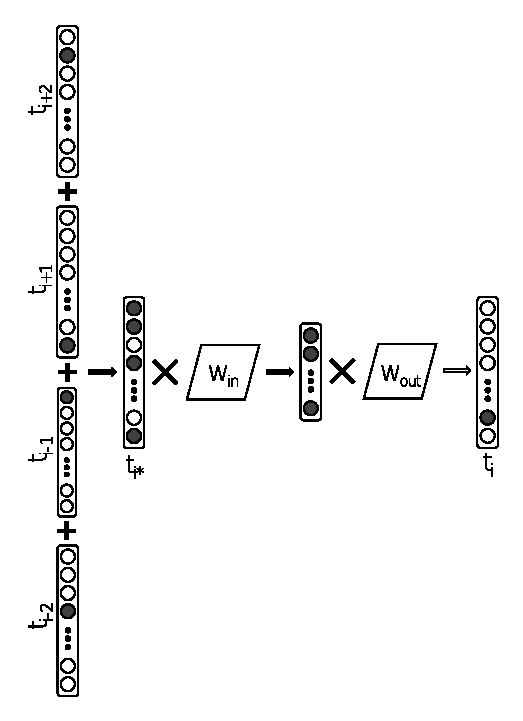
\includegraphics[scale=0.99]{Figures/CBOW_diagram.eps}
		\caption{Architecture of the C-BOW model \parentcite{mitra2018introduction}. The network attempts to predict a word given its context words. The order of input words is ignored. The hidden layer has much lower dimensionality in comparison to the one-hot representation of input and output words. The learned weights in $W_{in}$ (and $W_{out}$) can be used as word embeddings.}
		\label{chap:word_embeddingss:fig:CBOW_diagram}
	\end{center}
\end{figure}

%The generic architecture of the final output of the NLM described above is the equation \ref{chap:word_embeddingss:nlm_generic}. Note that the output vector $\vec{y}$ has size $|V|$ due to the input $\hat{w}$ and is the inference model of a \textit{continues distribution} of both the proximity of the words in the sentences (captured by the hidden layer) and the distribution over the vocabulary, which is the continues similarity of the words in this vocabulary. The output layer then is as described in equation \ref{chap:word_embeddings:eq:NLM}

%\begin{equation} \label{chap:word_embeddings:eq:NLM}
%	\vec{y} = \vec{t} + W_{out}(\vec{t}H + b_{h}) + b_{o}
%\end{equation}

%\noindent
%where $b_{o}$ and $b_{h}$ are the output and hidden layers biases. Usually the Hidden layer typically has a size of 500 to 1000 neurons while the projection layer might be 500 to 2000. Due to the multiple layers and the feeding of both the projection and the hidden to the output layer there is great complexity and the process is very computationally demanding. 

%A more efficient method is suggested in \parencite{mikolov2013efficient} where the non-linear hidden layer is removed and the projection layer is shared to all words, geometrically this is equivalent to the projection of the words to the same position. Then the algorithm is reformed and the $\hat{w}$ vectors are replaced by the $t^{*}$ which is the sum of the \textit{one-hot word vectors} \parencite{mitra2018introduction}. 

%Now the equation \ref{chap:word_embeddings:eq:NLM} is becoming \ref{chap:word_embeddings:eq:CBOW}. Due to the new form of the NNet where the tangent hidden layer is absent, there is no constraint in the presenting sequence of the words order. Moreover, the succeeding words also can also be taken in to account in a given \textit{window} say for $k_{w}$ number of words around the specific one. 

The weight matrix $W_{in}$ is of size $|V| \times m$ while $W_{out}$ is of size $m \times |V|$, where $m$ is the size of the hidden layer ($m << |V|$) and it also corresponds to the dimensionality of the extracted distributed representation. The size of the output vector is equal to the vocabulary size. 
%
%\begin{equation} \label{chap:word_embeddings:eq:CBOW}
%	\vec{y} = \hat{t}_{i*} \times W_{out} + b_{o}
%\end{equation}

During training, CBOW attempts to learn weight matrices $W_{in}$ and $W_{out}$. The loss function of CBOW is the following conditional log probability: 

\begin{equation} \label{chap:word_embeddings:eq:CBOW_log_likelihood}
	 \mathcal{L}_{CBOW} = -\frac{1}{|S|} \sum_{i=1}^{|S|}{\log{p(t_{i}|t_{i-k}, ... ,t_{i+k})}}
\end{equation}

\noindent
where $k$ is the size of context words and $S$ is the number of possible context windows in training texts. \textit{Stochastic Gradient Decent} and \textit{Backpropagation} are used to train that network. CBOW is actually an encoder-decoder model and applies a \textit{SoftMax} function in its output: 

\begin{equation} \label{chap:word_embeddings:eq:CBOW_softmax}
	p(t_{i}|t_{i-k},...,t_{i+k}) = \frac{e^{y_{t_{i}}}}{\sum^{|V|}_{i}{e^{y_{t_i}}}}
\end{equation}

\nointdent where $y_{t_i}$ is the output vector for term $t_i$.

Another architecture is the \textit{skip-gram} model, that attempts to predict the context of a word. This is depicted in figure \ref{chap:word_embeddingss:fig:skipgram_diagram} \parentcite{mitra2018introduction}. Again, input and output are one-hot vectors while the hidden layer is of dimensionality $m$ ($<<|V|$). The objective is to learn weight matrices $W_{in}$ and $W_{out}$ and the loss function is as follows:

\begin{equation} \label{chap:word_embeddings:eq:skipgram_log_likelihood}
	 \mathcal{L}_{SkipGram} = -\frac{1}{|S|} \sum_{i=1}^{|S|}{ \sum_{-k \leq j \leq +k}{ \log {p(t_{i+j}|t_{i})}  } }
\end{equation}

\nointend where $k$ is the number of context words to be predicted, $S$ the number of all windows in training set, and $p(t_{i+j}|t_{i})$ is obtained as follows:

\begin{equation} \label{chap:word_embeddings:eq:skipgram_softmax}
	p(t_{i+j}|t_{i}) = \frac{ e^{(W_{out}  \times  t_{i+j})^{T} (W_{in} \times  t_{i})}}{\sum^{|V|}_{k=1}{ e^{(W_{out}  \times  t_{k})^{T} (W_{in} \times  t_{i})}}} 
\end{equation}

\begin{figure}[t]
	\begin{center} 
    	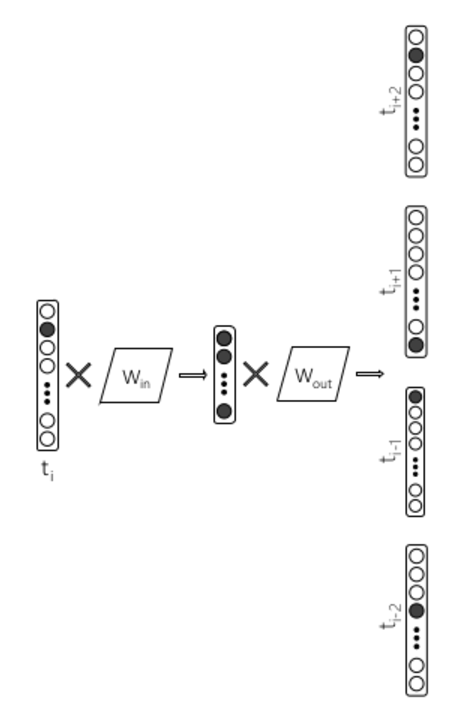
\includegraphics[scale=0.99]{Figures/skip_gram.eps}
		\caption{Architecture of skip-gram model \parentcite{mitra2018introduction}. Given a word the network tries to predict its context words. The dimensionality of the hidden layer is much lower than the one-hot representation of input and output words. The learned weights in $W_{in}$ (and $W_{out}$) can be used as word embeddings.}
		\label{chap:word_embeddingss:fig:skipgram_diagram}
	\end{center}
\end{figure}

Finally, the above neural models, either CBOW or skip-grams, since they are approximating the continuous distribution probability function of words over the the Vocabulary $V$ they also satify the following constraint:

\begin{equation} \label{chap:word_embeddings:eq:nnet_condtraint}
	\sum_{i=1}^{|V|}{p(t_{i}|t_{i-k}, ... ,t_{i+k})} = 1
\end{equation}

Note that in both CBOW and skip-gram models the two weight matrices $W_{in}$ and $W_{out}$ can be used to provide the word embeddings\footnote{An implementation of these methods is provided in https://github.com/tmikolov/word2vec}. Usually $W_{in}$ plays this role and $W_{out}$ is discarded.

%\textcolor{red}{THIS IS NOT CLEAR: A very important difference between the CBOW and skip-grams is the NNet architecture usually their implementation is based. Particularly, there are some internal detail occurring because of the objective of the task. \parencite{boden2002guide}}

To summarize, the above models are very effective \textit{Language Modeling} approaches having the ability to quantify simultaneously syntanctic and semantic information of words. They provide a \textit{distributed representation} for words (i.e., each word is represented with a dense vector which is a point in a space of relatively low dimensionality). However, it is not easy to understand the actual meaning of each dimension in this space. The sequence of words in texts is now considered and can also be applied in cases input texts are composed of sequences of characters or POS tags.

Finally, the training of the CBOW and the skip-gram models can be expensive despite the fact of limiting the number of hidden layers. However, there are several engineering solution that are accelerating the training time, such as \textit{Huffman binary tree encoding} of words and \textit{hierarchical softmax}. The latter is a solution that enables us to use multi-processing power and update the weight parameters concurrently. The parallel asynchronous updating of the parameter matrices is not conforming to the mathematical constraints however in practice the negative effect is minor. Huffman binary tree is a method for compressing the encoding of terms where the ones with the higher frequency are accessed faster. In addition to this, \textit{negative sampling}, \textit{sub-sampling}, or \textit{ramdom sampling} are also used where in the range of $k$ window for surrounding words only a few ones are selected during training with minor effect in  performance and significant acceleration in training \parentcite{mikolov2013efficient,mitra2018introduction}. 

\subsection{Document Embeddings} \label{chap:word_embeddings:sec:PVBOW} 
 
There are several approaches to transform word embeddings to document embeddings \parencite{mitra2018introduction,mikolov2013distributed}. The most simple method produces a vector for a given document by averaging the word embeddings of the words in a document. It is also possible to modify the network architecture and work on the sentence level. For example, word embeddings per sentence are averaged and the goal is to predict a sentence given its context sentences \parentcite{kenter2016}. Another idea, the \textit{Sent2Vec} method~\footnote{An implementation of this method can be found in https://github.com/epfml/sent2vec}, is to compose sentence embeddings by extending CBOW to include word vectors and word n-gram embeddings \parentcite{pagliardini-etal-2018-unsupervised}.

In this thesis, we use the \textit{Doc2Vec} approach, introduced in \parentcite{le2014distributed}, that attempts to generalize the word embeddings methods to work with sequences of words. The main idea is to train a neural network so that to learn embeddings for entire documents (or passages). There are two versions of this approach that are analogous to CBOW and skip-gram models. 

%\usepackage{authblk}

The \textit{Paragraph Vector - Distributed Memory} (PV-DV) model is based on CBOW. The task is to train a network to predict the next word in a text window given the paragraph vector and the word vectors of its context (actually the preceding words). The paragraph (it could be entire document) vector is considered as memory of the words distribution and aims to capture general information like the topic of the document. 

Another approach, following the skip-grams paradigm, is to ignore the context words in the input, and train a model for predicting a context word given its paragraph vector. This method, called \textit{Paragraph Vector - Distributed Bag-of-Words} (PV-DBOW), is depicted in figure \ref{chap:word_embeddingss:fig:PVBOW_diagram}. In practice, at each iteration of stochastic gradient descent, a text window of size $k$ is sampled. Then, a random word is sampled from the text window and form a classification task given the paragraph vector. This model requires to store less data, because only the SoftMax weights are stored as opposed to both SoftMax weights and word vectors in the PV-DM. 

The loss function of PV-DBOW (a modification of the corresponding skip-gram loss function shown in formula \ref{chap:word_embeddings:eq:skipgram_log_likelihood} is as follows: 

\begin{equation} \label{chap:word_embeddings:eq:pvbow_log_likelihood}
	 \mathcal{L}_{SkipGram} = -\frac{1}{|S|} \sum_{i=1}^{|S|}{ \sum_{-k \leq j \leq +k}{ \log {p(t_{i+j}|D_{i})}  } }
\end{equation}
\noindent
where $D_{i}$ is the document vector of $i$-th document, $S$ is the number of windows over the training texts and $k$ is the number of words to be predicted surrounding the input word. Consequently,  the SoftMax function for the output of the model is modified as follows:

\begin{equation} \label{chap:word_embeddings:eq:pvbow_softmax}
	p(t_{i+j}|t_{i}) = \frac{ e^{(W_{out}  \times  t_{i+j})^{T} (W_{in} \times  D_{i})}}{\sum^{|V|}_{i}{ e^{(W_{out}  \times  t_{k})^{T} (W_{in} \times  D_{i})}}} 
\end{equation}

\begin{figure}[t]
	\begin{center} 
      	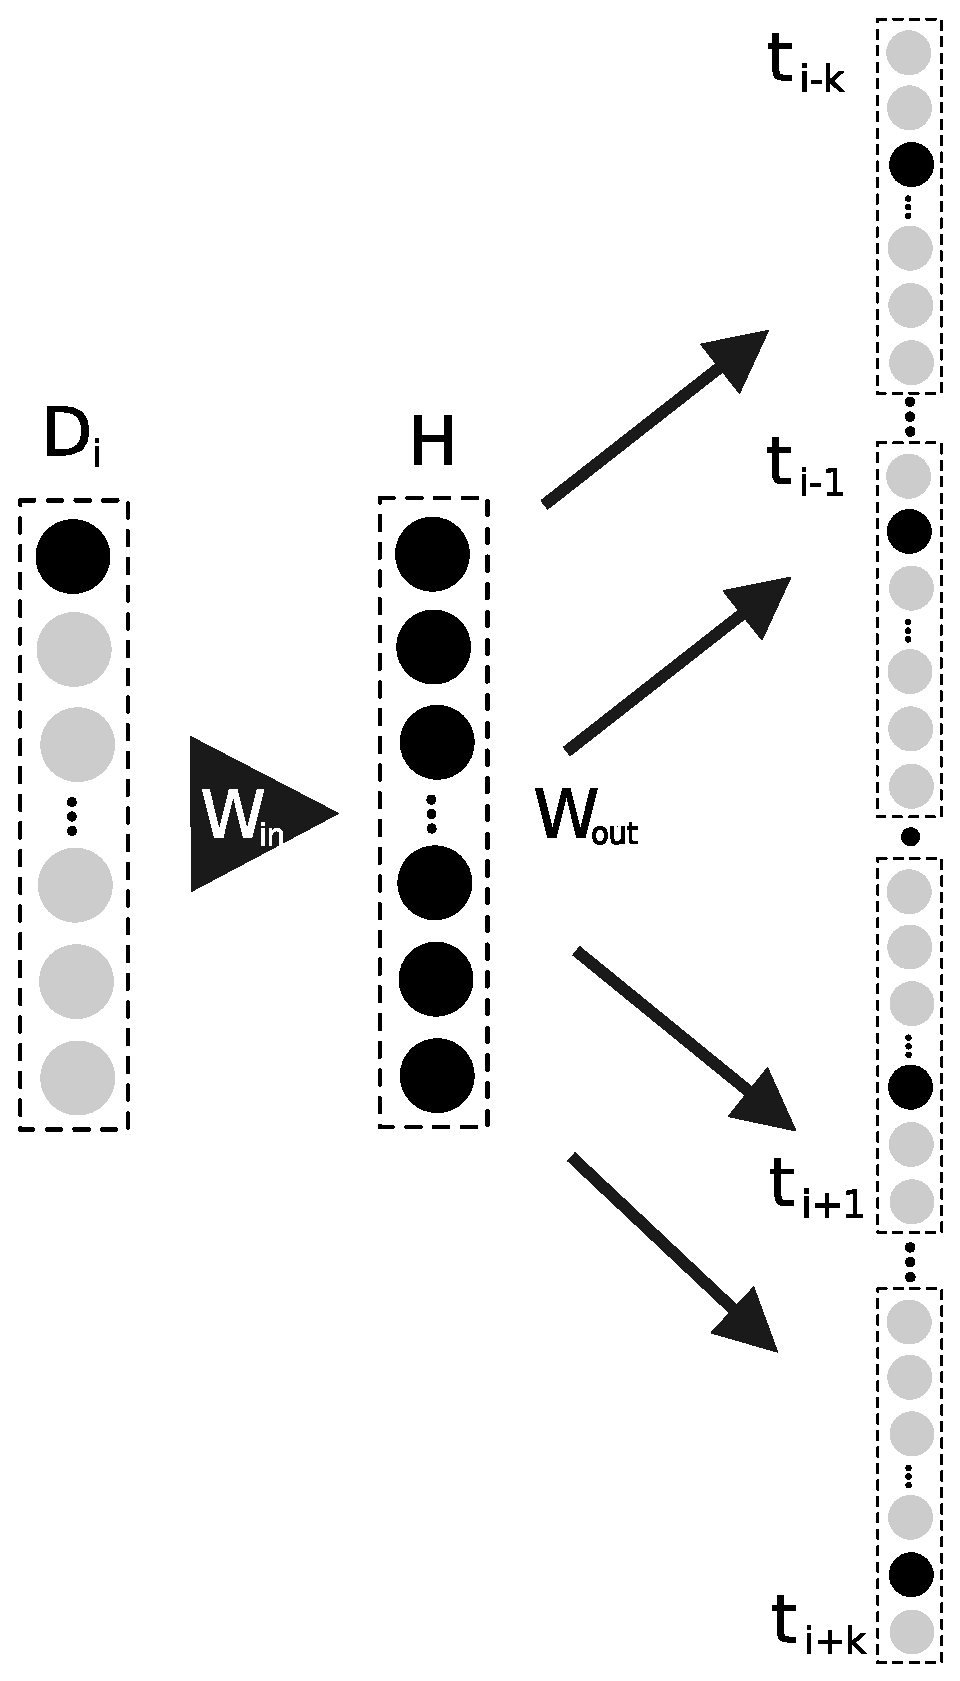
\includegraphics[scale=0.50]{Figures/pvbow.eps}
    		\caption{Architecture of PV-DBOW. Given a paragraph vector, predict context words.}
		\label{chap:word_embeddingss:fig:PVBOW_diagram}
	\end{center}
\end{figure}

There are several modifications for the PV-DBOW method aiming to increase its efficiency including, \textit{document frequency based negative sampling} and \textit{document length regularization} \parencite{le2014distributed,posadas2017application}. It should be noted that the paragraph vectors could be used to represent  sentences, paragraphs, or entire documents. In this study, the whole web-page is considered. In addition the input texts could be sequences of characters, POS tags, character n-grams, word n-grams etc.

This method of producing document embeddings has successfully been used in several text classification tasks \parentcite{le2014distributed}. Its main advantage over traditional BOW and n-gram representation schemes is that it provides compact and dense vectors that include a rich combination of syntactic semantic and stylistic information of documents.

\section{Experimental Setup}\label{chap:word_embeddings:sec:experiments_setup}

In this chapter, the usefulness of the previously described distributed representation of documents is examined in the framework of open-set WGI. As already explained, NNDR is vulnerable when combined with a text representation scheme of irrelevant and redundant features. In this thesis, NNDR is used in combination with \textit{Distributed Features} (DF), obtained by the PV-DBOW approach. We compare this new method with NNDR using traditional BOW and n-gram features as well as with other open-set methods (OCSVM and RFSE).

%\subsection{Corpus}\label{chap:word_embeddings:sec:experiments_corpora}

The experiments of this chapter are based on \textit{SANTINIS}, a benchmark corpus, as described in Chapter \ref{chap:noise}. Briefly, this dataset comprises 1,400 English web-pages evenly distributed into seven genres (blog, eshop, FAQ, frontpage, listing, personal home page, search page) as well as 80 BBC web-pages evenly categorized into four additional genres (DIY mini-guide, editorial, features, short-bio). In addition, the dataset comprises a random selection of 1,000 English web-pages taken from the SPIRIT corpus \parencite{joho2004spirit}. The latter can be viewed as \textit{unstructured noise} since genre labels are missing.

The PV-DBOW models have been trained using the whole corpus. Note that the training of this approach is unsupervised (i.e., the genre labels are not taken into account). The corpus initially is split to a set of paragraphs, as required from PV-DBOW. To be more specific, the paragraphs are sentences split from all the documents of the whole corpus. We examine three different variations, using either sequences of word unigrams (W1G), word trigrams (W3G) or character 4-grams (C4G) as input texts (W1G correspond to texts in their original form). Each type of n-grams is used separately as suggested in \parentcite{posadas2017application}. The dimensionality of document embeddings is selected from $DF_{dim}=\{50,100,250,500,1000\}$. 

In addition, the terms with very low-frequency in the training set are discarded. In this study, we examine $f_{min}=\{3,10\}$ as frequency cutoff threshold. The text window size is selected from $W_{size}=\{3,8,20\}$. The remaining parameters of PV-DBOW are set as follows: $\alpha=0.025$, $epochs=\{1, 3, 10\}$ and $decay=\{0.002, 0.02\}$. 

In practice, a library for HTML removal and and vector representation of the web-pages has been created for this work, named  \textit{Html2Vec}\footnote{\url{https://github.com/dpritsos/html2vec}}. There is a special module for PV-DBOW modeling that has been built based on the the implementation of the algorithm found in \textit{Gensim} package \footnote{\url{https://github.com/RaRe-Technologies/gensim}}. 

We also represent documents with traditional representation schemes to conduct comparative experiments. Similar to PV-DBOW, we extract regular C4G, W1G, and W3G. For each of these schemes, we use Term-Frequency weights (we use TF to refer to this kind of traditional feature as opposed to DF for distributed features). The feature space for TF is defined by a vocabulary $V_{TF}$, which is extracted based on the most frequent terms of the training set. We consider $V_{TF}=\{5k,10k,50k,100k\}$. 

Regarding the NNRD open-set classifier, there are two parameters, $lambda$ and DRT, and their considered values are: $\lambda =\{0.2, 0.5, 0.7\}$, $DRT\textit{=\{0.4, 0.6, 0.8, 0.9\}}$. All aforementioned parameters are adjusted based on grid-search using only the training part of the corpus.

%\textcolor{red}{STP and SUP values?}

The parameter tuning for OCSVM and RFSE methods has been performed as described in Chapter \ref{chap:noise} for the SANTINIS corpus. The reported evaluation results are obtained by performing 10-fold cross-validation and, in each fold, the full set of 1,000 noise pages is included. This evaluation strategy is giving a more realistic evaluation. Since the noise size is greater than the size of any known genre.

To compensate the unbalanced distribution of web pages over the genres because of the noise part, the open-set macro-averaged precision, recall, and $F_1$ measures are used \parentcite{mendesjunior2016}. Note again than this variant of evaluation measures ignores the unknown class.  

Finally, for selecting the parameter settings that obtain optimal evaluation performance, two scalar measures are used: the Area under the macro Precision-Recall Curve (AUC) of 11 standard Recall levels and the macro-averaged $F_{1}$ ($F_1^{macro}$) score.

\section{Experimental Results}\label{chap:word_embeddings:sec:results}

\subsection{The Effect of Distributed Representation on NNDR}\label{chap:word_embeddings:sec:NNDR_PVBOW_vs_BOW}

Initially NNDR is evaluated using the traditional TF scheme as shown in Table \ref{chap:word_embeddings:tbl:NNDR_TF}. The overall performance is poor. NNDR seems to work better with W3G features. Note that the dimensionality of this representation is quite high. The performance of the algorithm is slightly affected by parameter tuning for splitting ratios $p_1$ and $p_2$ while DRT in all cases is $0.8$. The method seems to be robust to the examined values of $\lambda$ regularization parameter. It should also be noted that both $F_1$ and AUC are maximized for the same parameter settings and document representation.

\begin{table}[t]
\center
\begin{tabular}{cccccccccc}
\hline
$p_1$ & $p_2$ & DRT & $\lambda$ & Features & Dim. & $P_{macro}$ & R_{macro} & $AUC_{macro}$ & $F_1^{macro}$ \\
\hline
0.7 & 0.3 & 0.8 & any & C4G & 5000 & 0.664 & 0.403 & 0.291 & 0.502 \\
0.7 & 0.5 & 0.8 & any & W1G & 5000 & 0.691 & 0.439 & 0.348 & 0.537 \\
0.5 & 0.5 & 0.8 & any & W3G & 10000 & \textbf{0.720} & \textbf{0.664} & \textbf{0.486} & \textbf{0.691} \\
\hline
\end{tabular}
\caption {Maximum performance of NNDR with traditional (TF) Features on SANTINIS coprus. $p_1$ and $p_2$ are the splitting ratios to form simulated noise and DRT is the threshold. $\lambda$ is the regulation parameter used in the normalized accuracy. Dim. is the dimensionality of representation. The evaluation measures are the open-set variants of macro-averaged precision, recall, $F_1$, and AUC of the precision-recall curve.}
\label{chap:word_embeddings:tbl:NNDR_TF}
\end{table}

\begin{table}
\center
\begin{tabular}{cccccccccc}
\hline
$p_1$ & $p_2$ & DRT & $\lambda$ & Features & Dim. & $P_{macro}$ & R_{macro} & $AUC_{macro}$ & $F_1^{macro}$ \\
\hline
any & any & 0.8 & any & C4G & 50 & \textbf{0.829} & 0.600 & 0.455 & 0.696 \\
any & any & 0.8 & any & W1G & 50 & 0.733 & \textbf{0.670} & 0.541 & 0.700 \\
any & any & 0.8 & any & W3G & 100 & 0.827 & 0.615 & \textbf{0.564} & \textbf{0.706} \\
\hline
\end{tabular}
\caption {Maximum performance of NNDR with distributed features on SANTINIS coprus. $p_1$ and $p_2$ are the splitting ratios to form simulated noise and DRT is the threshold. $\lambda$ is the regulation parameter used in the normalized accuracy. Dim. is the dimensionality of representation. The evaluation measures are the open-set variants of macro-averaged precision, recall, $F_1$, and AUC of the precision-recall curve.}
\label{chap:word_embeddings:tbl:NNDR_PVBOW}
\end{table}

The evaluation of NNDR combined with PV-DBOW features is shown in Table \ref{chap:word_embeddings:tbl:NNDR_PVBOW}. As can be seen, in two out of three types of features (C4G and W1G) the performance of the algorithm is significantly improved in terms of both macro $F_1$ and AUC. The best overall performance is still acquired by W3G features and it is slightly improved in comparison to the respective results when TF representation is used (the improvement is considerably higher for AUC measure). DF seems to particularly enhance precision results for C4G features and recall results for W1G features. 

These results are obtained using a much lower dimensionality of representation (i.e., an order of magnitude lower than TF scheme). This demonstrates that NNDR is better able to cope with the compactness and density of DF vectors. It should also be noted that the robustness of the model is increased since the best results are acquired for exactly the same parameter settings and most NNDR parameters do not affect the obtained performance. 

A more detailed view of the performance of NNDR when combined with either traditional or distributed W3G features is depicted in PRCs of Figure  \ref{chap:word_embeddings:fig:NNDR_W3G}. Note that in both cases the same parameter settings are used for the NNDR classifier.  As can be seen, the precision of the model based on DF remains high for more standard recall levels in comparison to TF which is significantly affected by the presence of noise. This means that DF is particularly useful in WGI applications where precision is considered more important than recall. The two approaches have comparable performance when recall reaches 0.5 although DF still outperforms TF. The points where curves stop indicate the percentage of the corpus that has been classified as unknown which is similar in both cases (i.e., about 40\% of the corpus).

\begin{figure}[t]

\begin{center}
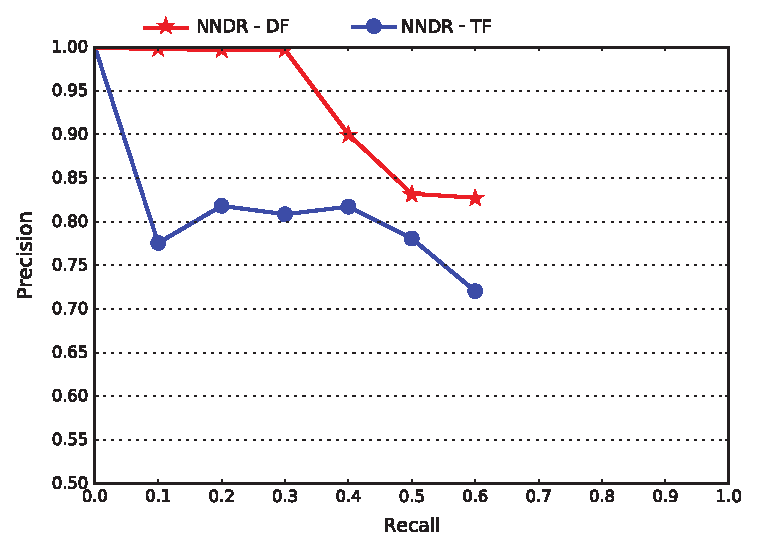
\includegraphics[scale=0.99]{Figures/NNDR_W3G.eps}
\caption{Precision-Recall curves of NNDR on SANTINIS corpus for traditional (TF) and distributed (DF) W3G features.}
\label{chap:word_embeddings:fig:NNDR_W3G}
\end{center}

\end{figure}

\subsection{Comparison of Open-set WGI Methods}\label{chap:word_embeddings:sec:experiments_setup}

In this section, the performance of NNDR on the SANTINIS corpus is compared to that of OCSVM and RFSE obtained as described in Chapter \ref{chap:noise}. The experimental setup for NNDR with either TF or DF schemes is exactly the same therefore the evaluation results for these models are directly comparable. In the framework of this experiment, OCSVM and RFSE serve as baseline models to help us see how competitive the NNDR approach can be when it is assisted by DF representation in unstructured noise conditions.

\begin{table}[t]
\center
\caption {Performance of baselines and NNDR on the SANTINIS coprus. All evaluation scores are macro-averaged.}
\label{chap:word_embeddings:tbl:NNDR_RFSE_OCSVME_final}
\begin{tabular}{ccccccc}
\hline
Model & Features & Dim. & Precision & Recall & AUC & F1 \\
\hline
RFSE & TF-C4G & 50k & 0.739 & \textbf{0.780} & 0.652 & 0.759 \\
RFSE & TF-W1G & 50k & 0.776 & 0.758 & \textbf{0.657} & \textbf{0.767} \\
RFSE & TF-W3G & 50k & 0.797 & 0.722 & 0.615 & 0.758 \\
OCSVM & TF-C4G & 5k & 0.662 & 0.367 & 0.210 & 0.472\\
OCSVM & TF-W1G & 5k & 0.332 & 0.344 & 0.150 & 0.338\\
OCSVM & TF-W3G & 10k & 0.631 & 0.654 & 0.536 & 0.643\\
NNDR & TF-C4G & 5k & 0.664 & 0.403 & 0.291 & 0.502 \\
NNDR & TF-W1G & 5k & 0.691 & 0.439 & 0.348 & 0.537 \\
NNDR & TF-W3G & 10k & 0.720 & 0.664 & 0.486 & 0.691 \\
NNDR & DF-C4G & 50 & \textbf{0.829} & 0.600 & 0.455 & 0.696 \\
NNDR & DF-W1G & 50 & 0.733 & 0.670 & 0.541 & 0.700 \\
NNDR & DF-W3G & 100 & 0.827 & 0.615 & 0.564 & 0.706 \\
\hline
\end{tabular}
\end{table}

First, NNDR with TF features is compared with the baselines. In this case, NNDR outperforms OCSVM. On the other hand, RFSE performed NNDR in both macro-averaged $F_1$ and AUC. This is consistent for any kind of features (C4G, W1G, or W3G). The RFSE model is the top overall performer while both OCSVM and NNDR are significantly low in respect of AUC, $F_1$ and precision. Only, NNDR with TF scheme for W3G is competitive. 

There is notable difference in the dimensionality of representation used by the examined approaches though. RFSE relies upon a 50k-manifold while NNDR and OCSVM are based on much lower dimensional spaces. This demonstrates the ability of RFSE to exploit the existence of redundant feature sets. It has to be noted that RFSE builds an ensemble by iteratively and randomly selecting a subset of the available features. That way, it internally reduces the dimensionality for each constituent base classifier (RFSE is using 1,000 randomly selected features from the 50,000 most frequent features in each repetition). 

Next, NNDR with DF is compared with the same baselines. Although there is a notable improvement for NNDR using DF, it is still outperformed by RFSE in terms of both $F_1$ and AUC. On the other hand, NNDR returns a notably higher performance than RFSE with respect to precision for C4G and W3G features. This indicates that NNDR using DF could be more useful than RFSE in WGI applications where precision is more important than recall.

A closer look at  the comparison of the examined methods is provided in Fig. \ref{chap:word_embeddings:fig:NNDR_W3G_Best_RFSE_Baseline}, where macro-averaged precision-recall curves are depicted. The NNDR-DF model maintains very high precision scores for low levels of recall. Particularly, for W3G features the difference between NNDR-DF and RFSE at that point is clearer. NNDR-TF is clearly worse than both NNDR-DF and RFSE. In addition, OCSVM is competitive in terms of precision only when W3G features are used but its performance drops abruptly in comparison to that of NNDR-DF. 

RFSE with W1G performs significantly better in terms of precision than NNDR (with DF). It also manages to recognize correctly larger part of the corpus, more than $70\%$ either for W3G or for W1G, as compared to NNDR-DF that reaches $60\%$ in both cases. 

\begin{figure}[t]
\begin{center}
    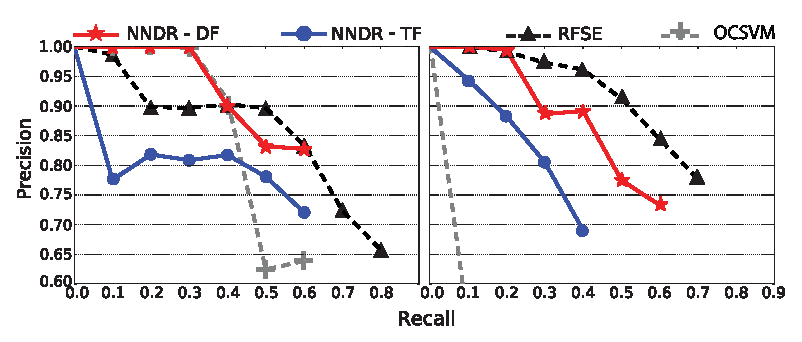
\includegraphics[scale=0.95]{Figures/NNDR_W3G-W1G_Best_RFSE-OCSVM-Baselines.eps}
	\caption{Precision curves in 11-standard recall levels of the examined open-set classifiers using either W3G features (left) or W1G features (right).}
	\label{chap:word_embeddings:fig:NNDR_W3G_Best_RFSE_Baseline}
	\end{center}
\end{figure}

%, i.e. the remaining part after the last mark of each curve it the percentage of the corpus tha has been classified as Unknown from the algorithms.

\section{Conclusions}\label{chap:word_embeddings:sec:conclusions}

In this chapter, we presented an experimental study focused on WGI and the use of distributed features in combination with an open-set classifier that obtained promising results in other domains \parentcite{mendesjunior2016}. Our experiments are based on a benchmark corpus with unstructured noise already used in previous work and a strong baseline. 

It seems that distributional features provide a significant enhancement to the performance of NNDR in WGI tasks. The low-dimensionality and density of DF are crucial to enhance the performance of NNDR which suffers from the presence of irrelevant and redundant features (as any nearest-neighbor method). Yet, RFSE proves to be a hard-to-beat baseline at the expense of relying upon a much higher representation space (usually in the thousands of features). However, with respect to precision, NNDR with PV-DBOW features is much more conservative and it prefers to leave web-pages unclassified rather than predicting an inaccurate genre label. Depending on the application of WGI, precision can be considered much more important than recall and this is where the proposed approach seems more suitable (e.g., web-page ranking applications).

Further research could focus on more appropriate distance measures within NNDR specially with recent data-driven features obtained with powerful NLP convolutional and recurrent deep networks. Moreover, alternative types of distributed features could be used (e.g., topic modeling or pre-trained language models). Finally, a combination of NNDR with RFSE models could be studied as they seem to exploit complementary views of the same problem.


%!TeX spellcheck = en-US

\chapter{Conclusions}

\label{chap:conclusions}

%----------------------------------------------------------------------------------------

% Define some commands to keep the formatting separated from the content
\newcommand{\keyword}[1]{\textbf{#1}}
\newcommand{\tabhead}[1]{\textbf{#1}}
\newcommand{\code}[1]{\texttt{#1}}
\newcommand{\file}[1]{\texttt{\bfseries#1}}
\newcommand{\option}[1]{\texttt{\itshape#1}}

%----------------------------------------------------------------------------------------




%----------------------------------------------------------------------------------------
%	BIBLIOGRAPHY
%----------------------------------------------------------------------------------------
\printbibliography[heading=bibintoc]


\end{document}
